\documentclass[10pt,a4paper]{article}
\usepackage[latin1]{inputenc}
% \usepackage{amsmath}
\usepackage{amsfonts}
% \usepackage{amssymb}
\usepackage{amsmath,amsthm,amssymb}
\usepackage{graphicx}
\usepackage{hyperref}
% \usepackage{courier}
\usepackage{placeins}
\usepackage{fancyhdr}
\usepackage{color}
% \usepackage{xcolor}
\usepackage{listings}
\usepackage{geometry}
\usepackage{tabularx}
\usepackage[table]{colortbl}
\usepackage{placeins}
% \usepackage{cite}
\usepackage{subcaption}
\usepackage{lipsum}
\usepackage{titlesec}
\usepackage{dsfont}
\usepackage{parskip}
\usepackage{soul}
\usepackage[backend=biber]{biblatex}
\addbibresource{mybib.bib}
\usepackage[skip=8pt,labelfont=bf, font=sf]{caption}
	\DeclareCaptionFont{myfont}{\fontfamily{\sfdefault}\selectfont}

\hypersetup{
	colorlinks   = True,
	citecolor    = blue,
	linkcolor	 = blue,
}

% \geometry{letterpaper, portrait, margin=1in}
% \geometry{a4paper,margin=15mm,bindingoffset=25mm,heightrounded,}
\geometry{a4paper,margin=25mm}

\usepackage[dvipsnames]{xcolor}
\definecolor{lightgray}{rgb}{.93,.93,.93}
\definecolor{darkgray}{rgb}{.4,.4,.4}
\definecolor{purple}{rgb}{0.65, 0.12, 0.82}

\usepackage{helvet}
\usepackage{times}

\titleformat{\chapter}[display]
  {\normalfont\sffamily\huge\bfseries} % \color{blue}
  {\chaptertitlename\ \thechapter}{20pt}{\Huge}
\titleformat{\section}
  {\normalfont\sffamily\huge\bfseries} % \color{cyan}
  {\thesection}{1em}{}
 \titleformat{\subsection}
  {\normalfont\sffamily\Large\bfseries} % \color{cyan}
  {\thesubsection}{1em}{}
 \titleformat{\subsubsection}
  {\normalfont\sffamily\large\bfseries} % \color{cyan}
  {\thesubsubsection}{1em}{}
\renewenvironment{abstract}
 {\par\noindent\Huge\textbf{\abstractname.}\\\vspace{1em}\ignorespaces}
 {\par\medskip} 

% \renewcommand*\abstractname{Abstract\hfill}
% \renewcommand{\familydefault}{\sfdefault}


\def \lineheight {1.5pt}

\makeatletter
   \def\vhrulefill#1{\leavevmode\leaders\hrule\@height#1\hfill \kern\z@}
\makeatother

\usepackage{caption}
    \DeclareCaptionType{mycapequ}[][List of equations]
    \captionsetup[mycapequ]{labelformat=empty}

\usepackage{inconsolata}

\lstset{
	language=Matlab,
	backgroundcolor=\color{lightgray},
	keywordstyle=\color{blue}\bfseries,
	stringstyle=\color{red}\ttfamily,
	commentstyle=\color{ForestGreen}\ttfamily,
	identifierstyle=\color{black},
	extendedchars=true,
	% basicstyle=\footnotesize\ttfamily,
	basicstyle=\normalsize\fontencoding{T1}\ttfamily,
	showstringspaces=false,
	showspaces=false,
	numbers=left,
	numberstyle=\footnotesize,
	numbersep=9pt,
	tabsize=2,
	breaklines=true,
	showtabs=false,
	captionpos=b
}

\lstset{
	language=Python,
	backgroundcolor=\color{lightgray},
	keywordstyle=\color{blue}\bfseries,
	stringstyle=\color{red}\ttfamily,
	commentstyle=\color{ForestGreen}\ttfamily,
	identifierstyle=\color{black},
	extendedchars=true,
	% basicstyle=\footnotesize\ttfamily,
	basicstyle=\normalsize\fontencoding{T1}\ttfamily,
	showstringspaces=false,
	showspaces=false,
	numbers=left,
	numberstyle=\footnotesize,
	numbersep=9pt,
	tabsize=2,
	breaklines=true,
	showtabs=false,
	captionpos=b
}

\fancypagestyle{firstpage}{%
  \fancyhf{}% clear default for head and foot
  % \rfoot{\textbf{Page \thepage}}
  % \lfoot{\textbf{\today}}
  \renewcommand{\headrulewidth}{0pt}
}
\fancypagestyle{blank}{%
	\fancyhf{}
	\renewcommand{\headrulewidth}{0pt}
}

\fancypagestyle{nohdr}{%
	\fancyhf{}
	\renewcommand{\headrulewidth}{0pt}
	\rfoot{\fontfamily{\sfdefault}\selectfont\textbf{Page \thepage}}
}

\renewcommand{\headrulewidth}{1pt}% 2pt header rule


% \fontfamily{\sfdefault}\selectfont
	% \large\fontfamily{\rmdefault}\selectfont 

\setlength{\parskip}{12pt} % 1ex plus 0.5ex minus 0.2ex}
\setlength{\parindent}{0pt}

\pagestyle{fancy}
% \renewcommand{\sectionmark}[1]{\markboth{ #1}{}}
% \renewcommand{\subsectionmark}[1]{\markboth{\thesection\ #1}{\thesubsection\ #1}}
\fancyhf{}
\rhead{\fontfamily{\sfdefault}\selectfont \textbf{\rightmark}}
\lhead{\fontfamily{\sfdefault}\selectfont \textbf{Specialization Project}}
\rfoot{\fontfamily{\sfdefault}\selectfont \textbf{Page \thepage}}
\lfoot{\fontfamily{\sfdefault}\selectfont \textbf{Cole Nielsen}} % \today

\title{\textbf{}}
\date{}

\sloppy\raggedright
\begin{document}	
		% \maketitle 
	% \renewcommand{\familydefault}{\sfdefault}
	\thispagestyle{firstpage}
	\fontfamily{\sfdefault}\selectfont 
	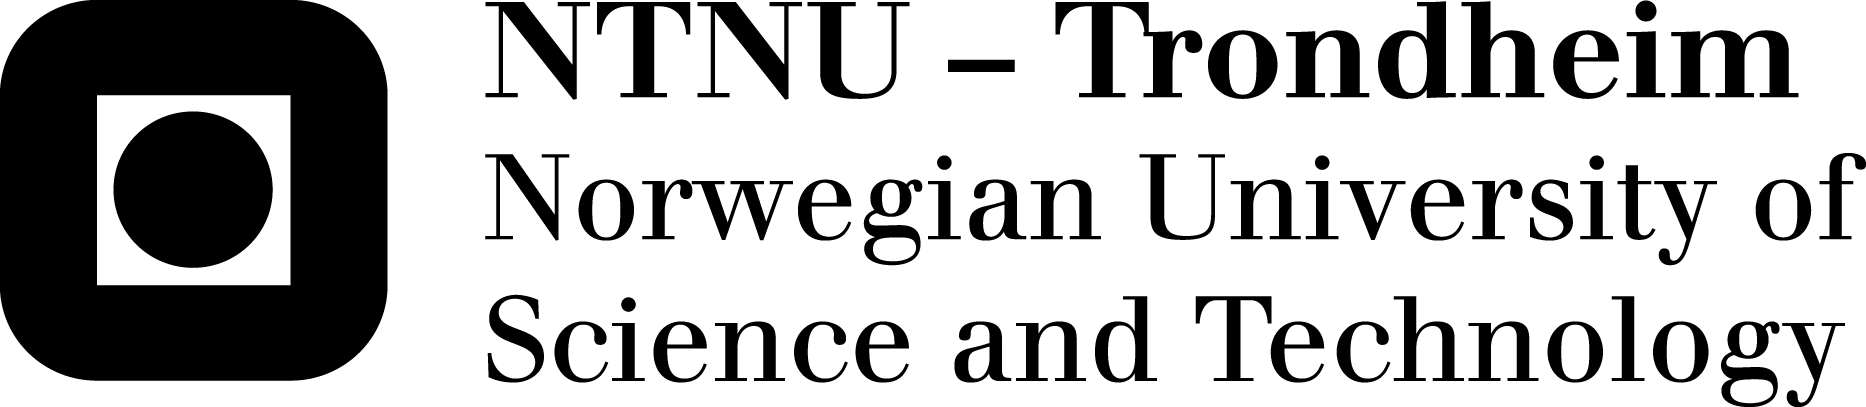
\includegraphics[width=0.5\linewidth]{logo_ntnu_eng_black.png} \\
	\vspace{8em}
	\huge Python Framework for Design and Simulation of Integer-N ADPLLs\\	
	\vspace{3em}
	\huge \textbf{Cole Nielsen}\\
	\vspace{12em}
	\large
	Electronic Systems Design, Specialization Project\\
	\vspace{4pt}
	\FloatBarrier

	\def\arraystretch{1.3}
	\setlength{\tabcolsep}{1em}
	\begin{tabular}{@{} l  l}
	Submission date: & December 2019\\
	Supervisor: & Trond Ytterdal, IET\\
	Co-supervisor: & Carsten Wulff, IET\\
	\end{tabular} \\
	\FloatBarrier
	\vspace{3em}
	Norwegian University of Science and Technology \\ 
	\vspace{4pt}Department of Electronic Systems\\
	
	% \begin{center}
	% 	\large
	% 	\begin{tabular}{ l r }
	% 		\textbf{Name} & Cole Nielsen \\
	% 		\textbf{Assigned N$^\textbf{\textnormal{o}}$} & 13 \\
	% 		\textbf{Term} & Autumn 2018\\
	% 		\textbf{Instructor} & Guennadi Kouzaev\\
	% 	\end{tabular}
	% \end{center}
	% \vspace{2em}
	% \vhrulefill{\lineheight}
	\pagebreak
	\thispagestyle{blank}
	\null\pagebreak

	% % % % % % % % % % % % % % % % % % % % % % % % % % % % % % % % % % % % 
	% Abstract		
	\setcounter{page}{1}
	\pagebreak
	\thispagestyle{nohdr}
	\begin{abstract}
		\large\fontfamily{\rmdefault}\selectfont 
		An open source Python-language design automation and simulation framework for the design of integer-N all digital phase locked loop (ADPLL) frequency synthesizers is presented in this paper. The framework enables (1) automatic design of optimized second order discrete time digital loop filters, and (2) behavioral ADPLL simulation to verify loop filter and PLL designs for satisfactory phase noise, lock-time and stability; optionally subject to variation using Monte-Carlo sampling. Simulation is implemented with a discrete-event time domain simulator utilizing behavioral PLL component models, permitting accurate modeling of effects of time-discretization and quantization in an ADPLL. Loop filter design automation is based upon a prototype second order filter, whose parameters are optimized to minimize total integrated output phase noise for a PLL provided specifications for reference frequency, divider ratio, time-to-digital converter (TDC) resolution, digitally controlled oscillator (DCO) gain, oscillator phase noise characteristics and maximum lock time. The optimizer utilizes continuous phase transfer function approximation of ADPLL dynamics and phase noise, which allows for computationally fast evaluation, but also requires conversion of the design filters from continuous-to-discrete time. Second order optimization is utilized post filter design to map the discrete filter into a fixed-point digital with acceptable quantization noise and filter error due to quantization effects.
	\end{abstract}
	% \section*{Abstract}
	% fjdsfkajjlkf

	% % % % % % % % % % % % % % % % % % % % % % % % % % % % % % % % % % % % 
	% Project Description
	\pagebreak
	\thispagestyle{nohdr}
	\null\pagebreak
	\thispagestyle{nohdr}
	\Huge\textbf{Problem description.}\\
	\vspace{1em}
	\large\fontfamily{\rmdefault}\selectfont 
	
	The intent of this project is to develop a standalone PLL design and simulation framework to aid and facilitate a later master's thesis project regarding the design of an all-digital, ultra-low power PLL frequency synthesizer. This framework is intended to address and ease all-digital PLL design and simulation challenges at a high level. Specifically it should enable speedy PLL simulation defined with system and component- level specifications (e.g. desired frequency, gain of digitally controlled oscillator, phase detector resolution, divider ratio). This is to allow for development of component level specifications and verification of PLL performance (phase noise, lock time, stability) under ideal circumstances before transistor level implementation, thus accelerating overall implementation time for hardware.

	% % % % % % % % % % % % % % % % % % % % % % % % % % % % % % % % % % % % 
	% % Preface
	% \pagebreak
	% \thispagestyle{nohdr}
	% \null\pagebreak
	% \thispagestyle{nohdr}
	% \large\fontfamily{\sfdefault}\selectfont 
	% \Huge\textbf{Preface.}\\
	% \vspace{1em}
	% \large\fontfamily{\rmdefault}\selectfont 
	% \lipsum[1]

	% % % % % % % % % % % % % % % % % % % % % % % % % % % % % % % % % % % % 
	% Contents, list of tables and figures
	\fontfamily{\sfdefault}\selectfont 
	\thispagestyle{nohdr}
	\null\pagebreak
	\thispagestyle{nohdr}
	\null\pagebreak
	\tableofcontents
	\pagebreak
	\listoffigures
	\listoftables

	% \vhrulefill{\lineheight}

	\fontfamily{\rmdefault}\selectfont 
	% % % % % % % % % % % % % % % % % % % % % % % % % % % % % % % % % % % % 
	% Abbreviations
	\section*{Abbreviations.}
	\begin{table}[htb!]
	\renewcommand*{\arraystretch}{1.45}\large
	\begin{tabular}{@{}ll}
		\textbf{\textsf{ADPLL}}	&	All digital phase locked loop \\
		\textbf{\textsf{AR}}	&	Autoregressive \\
		\textbf{\textsf{BBPD}}	&	Bang-bang phase detector \\
		\textbf{\textsf{BW}}	&	Bandwidth \\
		\textbf{\textsf{CI}}	&	Confidence interval \\
		\textbf{\textsf{CLK}}	&	Clock \\
		\textbf{\textsf{CMOS}}	&	Complementary metal oxide semiconductor \\
		\textbf{\textsf{DCO}}	&	Digitally controlled oscillator \\
		\textbf{\textsf{DFT}}	&	Discrete Fourier transform \\
		\textbf{\textsf{DIV}}	&	Divider \\
		\textbf{\textsf{FFT}}	&	Fast Fourier transform \\
		\textbf{\textsf{GSS}}	&	Golden section search \\
		\textbf{\textsf{IIR}}	&	Infinite impulse response \\
		\textbf{\textsf{KDCO}}	&	DCO Gain \\
		\textbf{\textsf{LF}}	&	Loop filter \\
		\textbf{\textsf{LSB}}	&	Least significant bit \\
		\textbf{\textsf{MMSE}}	&	Minimum mean squared error \\
		\textbf{\textsf{MSE}}	&	Mean squared error \\
		\textbf{\textsf{NF}}	&	Noise figure \\
		\textbf{\textsf{OTW}}	&	Oscillator tuning word \\
		\textbf{\textsf{PD}}	&	Phase detector \\
		\textbf{\textsf{PI}}	&	Proportional-integral \\
		\textbf{\textsf{PID}}	&	Proportional-integral-derivative \\
		\textbf{\textsf{PLL}}	&	Phase locked loop \\
		\textbf{\textsf{PM}}	&	Phase margin \\
		\textbf{\textsf{PSD}}	&	Power spectral density \\
		\textbf{\textsf{PVT}}	&	Process, voltage and temperature \\
		\textbf{\textsf{RMS}}	&	Root mean squared \\
		\textbf{\textsf{SFDR}}	&	Spurious free dynamic range \\
		\textbf{\textsf{TDC}}	&	Time to digital converter \\
		\textbf{\textsf{TF}}	&	Transfer function \\
		\textbf{\textsf{VCO}}	&	Voltage controlled oscillator \\
	\end{tabular}
	\end{table}


	% % % % % % % % % % % % % % % % % % % % % % % % % % % % % % % % % % % % 
	\pagebreak
	\FloatBarrier

	\section{Introduction}\label{intro}
	\section{Introduction}\label{intro}
Phase locked loops are extraordinarily useful frequency synthesizers that are vital to the operation of virtually all wired and wireless communication systems of today. The trend towards increasingly lower power wireless devices poses an acute need to reduce PLL power consumption. This is a challenge as PLLs typically rank among the highest power consuming components of a radio, and are necessarily so to limit phase noise. Reducing analog PLL power consumption can be a prohibitive challenge as the performance of analog loop filters degrade as a result of unavoidably lower charge pump current. However, recent CMOS process nodes with minimum gate lengths as small as 7nm allow for all-digital PLLs as an attractive alternative to analog designs due to low power consumption associated with the implementation of a digital loop filter. Digital loop-filters have a unique advantage where they can be scaled indefinitely as process nodes advance, while suffering no loss in performance. 

All-digital PLLs introduce new challenges in the process of design in the ultra-low power domain. Low power design is complemented by low complexity design, which in a PLL transcribes to low resolution of phase detectors, digitally tunable oscillators, and loop filter digital data paths. In other words, effects of quantization are strong. Whereas analog designs and high power/resolution digital designs can be effectively analyzed (even by hand) with transfer functions in the Z-domain, time domain simulation is necessary to capture quantization effects in low power, low resolution ADPLLs. This, of course, presents a challenge in manual design of PLLs if simulation is an integral part to the most basic modeling, and thus motivates the creation of an automated design solution. Currently, no PLL design framework is known that automates PLL design for the needs of ultra low power PLLs as characterized here. Of the most prominent pre-existing frameworks, CppSim \hl{[add reference...]} features a utility for design of continuous loop filters, however for this it does not provide any level of performance optimization, nor does it support discrete-time and quantized digital designs. 

Thus in this paper, a new framework written in pure-Python is introduced, which uniquely addresses issues of ultra-low power ADPLL design. Specifically, design of integer-N type PLLs is focused on, as the impetus of this work is an integer-N PLL design project. Topics presented are (a) automatic design and optimization of ADPLL loop filters given target system and component level specs for the PLL, and (b) behavioral time domain PLL simulation for accurate analysis and verification of PLL performance, with an integrated Monte-Carlo sampling variation analysis engine.

A brief outline of the paper is as follows. An introduction to PLL theory is in section \ref{theory}. Simulation and optimization methods are discussed in section \ref{methods}. An example design exercise, a comparison to existing solutions, and general discussion considerations for using the framework are in section \ref{disco}. Finally, section \ref{conclusion} concludes.

\hl{include main contributions}
	\pagebreak
	\FloatBarrier

	\section{Theory}\label{theory}
	\section{Theory}\label{theory}
	In its most basic form, a phase locked loop is a phase-based feedback system whose output tracks or maintains a fixed phase relationship to an input signal. Such a system is uniquely suited to the task of frequency synthesis, which is the process of generating derivative frequencies from some reference frequency. Given reference and output phase signals $\Phi_{ref}$ and $\Phi_{out}$, a PLL can be modeled as in figure \ref{fig:basic_fb}, with feedforward and feedback networks A(s) and B(s). 
	\begin{figure}[htb!]
		\center\fontfamily{\sfdefault}\selectfont
% XCircuit output "basic_feedback.tex" for LaTeX input from basic_feedback.ps
\def\putbox#1#2#3#4{\makebox[0.00000in][l]{\makebox[#1][l]{}\raisebox{\baselineskip}[0.00000in][0.00000in]{\raisebox{#2}[0.00000in][0.00000in]{\scalebox{#3}{#4}}}}}
\def\rightbox#1{\makebox[0.00000in][r]{#1}}
\def\centbox#1{\makebox[0.00000in]{#1}}
\def\topbox#1{\raisebox{-0.60\baselineskip}[0.00000in][0.00000in]{#1}}
\def\midbox#1{\raisebox{-0.20\baselineskip}[0.00000in][0.00000in]{#1}}
   \scalebox{1}{
   \normalsize
   \parbox{3.61667in}{
   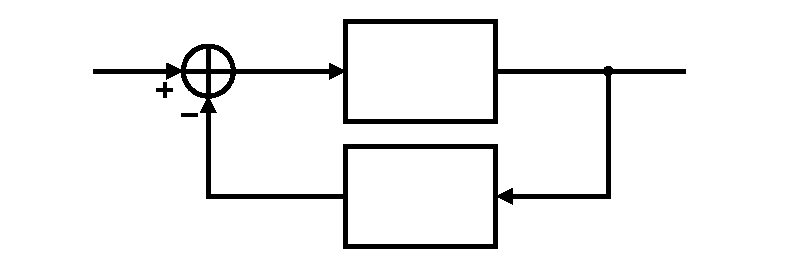
\includegraphics[scale=0.70000]{./figs/basic_feedback.pdf}\\
   % translate x=544 y=496 scale 0.38
   \putbox{1.82000in}{0.85400in}{1.20}{A(s)}%
   \putbox{1.82000in}{0.27300in}{1.20}{B(s)}%
   \putbox{0.44800in}{1.00100in}{1.20}{$\Phi_{ref}$}%
   \putbox{2.84200in}{1.00100in}{1.20}{$\Phi_{out}$}%
   \putbox{1.12000in}{1.00100in}{1.20}{$\Phi_{error}$}%
   } % close 'parbox'
   } % close 'scalebox'
   \vspace{-\baselineskip} % this is not necessary, but looks better
\fontfamily{\rmdefault}\selectfont

		\caption{Basic phase feedback network.}
		\label{fig:basic_fb}
	\end{figure}
	\FloatBarrier
	The closed loop phase response T(s) for $\Phi_{ref}$ to $\Phi_{out}$ is therefore:
	\begin{equation}
		\mathrm{T}(s) = \frac{\Phi_{out}(s)}{\Phi_{ref}(s)} = \frac{A(s)}{1+A(s)B(s)}
	\end{equation}
	A particular case of interest is when B(s) = 1/N, where N is a constant, and the loop gain A(s)B(s) $>>$ 1, the closed loop response is:
	\begin{equation}\label{mult_by_n}
		\frac{\Phi_{out}(s)}{\Phi_{ref}(s)} \approx \frac{A(s)}{A(s)B(s)} = \frac{1}{B(s)} = N
	\end{equation}
	We see that the phase through the PLL is multiplied by a factor of N. If the input phase signal is a sinusoid with frequency $\omega_{ref}$, and likewise the output with $\omega_{out}$, then $\phi_{ref}(t)=\omega_{ref}t$ and $\phi_{out}(t)=\omega_{out}t$. Thus:
	\begin{equation}\label{mult_by_n}
		\frac{\Phi_{out}}{\Phi_{ref}} = \frac{\omega_{out}t}{\omega_{ref}t} \approx N \hspace{1em} \rightarrow \hspace{1em} \omega_{out} \approx N\omega_{ref}
	\end{equation}
	Therefore, it is observed that a PLL allows for the generation, i.e. synthesis, of a new frequency from a reference frequency signal. Given a feedback divider ration of 1/N, the PLL multiplies the reference frequency by a factor of N. In the following sections, more advanced models for PLL will be developed, extending the concept introduced here. Specifically, the theory of digital, discrete-time PLLs will be developed and extended from a continuous phase model of a basic PLL.

	\subsection{Continuous PLL Model}
		Although PLLs are practically limited to using discrete-time sampling in real-word hardware, continuous models can still be applied in their analysis and design. Thus a continuous PLL model is developed in this section to aid in the later discussed discretized PLL modeling.

		\subsubsection{PLL Synthesizer architecture}
			The traditional architecture for implementing a PLL frequency synthesizer \cite{Razavi1996DesignOM} is shown in figure \ref{fig:basic_pll}. This basic PLL is comprised of four components: (1) a phase detector, denoted by PD, (2) a loop filter, denoted by H$_{LF}$(s), (3) a voltage controlled oscillator, denoted by VCO, and (4) and phase divider, denoted by "$\div$ N" in the figure. These components are explained in the following sections.
			\begin{figure}[htb!]
				\center\fontfamily{\sfdefault}\selectfont
% XCircuit output "basic_pll.tex" for LaTeX input from basic_pll.ps
\def\putbox#1#2#3#4{\makebox[0.00000in][l]{\makebox[#1][l]{}\raisebox{\baselineskip}[0.00000in][0.00000in]{\raisebox{#2}[0.00000in][0.00000in]{\scalebox{#3}{#4}}}}}
\def\rightbox#1{\makebox[0.00000in][r]{#1}}
\def\centbox#1{\makebox[0.00000in]{#1}}
\def\topbox#1{\raisebox{-0.60\baselineskip}[0.00000in][0.00000in]{#1}}
\def\midbox#1{\raisebox{-0.20\baselineskip}[0.00000in][0.00000in]{#1}}
   \scalebox{1}{
   \normalsize
   \parbox{4.49167in}{
   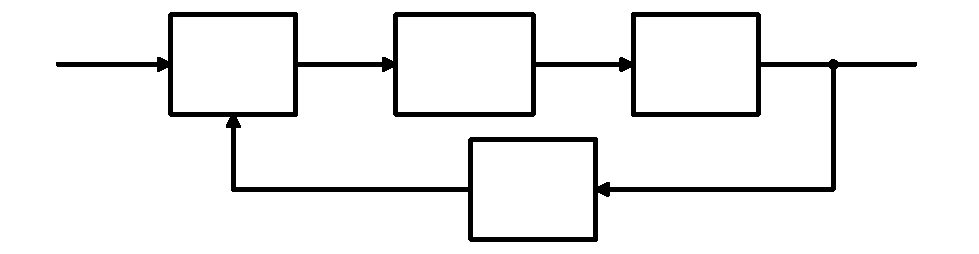
\includegraphics[scale=0.70000]{./figs/basic_pll.pdf}\\
   % translate x=320 y=488 scale 0.38
   \putbox{0.97300in}{0.82600in}{1.20}{PD}%
   \putbox{2.34500in}{0.24500in}{1.20}{$\div$ N}%
   \putbox{0.32900in}{0.97300in}{1.20}{$\Phi_{ref}$}%
   \putbox{3.71700in}{0.97300in}{1.20}{$\Phi_{out}$}%
   \putbox{1.90400in}{0.82600in}{1.20}{H$_{LF}$(s)}%
   \putbox{3.07300in}{0.82600in}{1.20}{VCO}%
   \putbox{1.49800in}{0.39200in}{1.20}{$\Phi_{div}$}%
   \putbox{1.52600in}{0.97300in}{1.20}{$\Phi_e$}%
   \putbox{2.54800in}{0.97300in}{1.20}{V$_{ctrl}$}%
   } % close 'parbox'
   } % close 'scalebox'
   \vspace{-\baselineskip} % this is not necessary, but looks better
\fontfamily{\rmdefault}\selectfont

				\caption{Basic PLL.}
				\label{fig:basic_pll}
			\end{figure}
			\FloatBarrier

		\subsubsection{Divider}
			The phase divider is used as the feedback path in the PLL, where the division modulus N controls the frequency multiplication of the PLL. The tranfer function of the divider is:
			\begin{equation}
				\mathrm{H}_{div}(s) = \frac{\Phi_{div}(s)}{\Phi_{out}(s)} = \frac{1}{\mathrm{N}}
			\end{equation}

			\subsubsection{Phase detector}
			The phase detector is used to measure the phase of the feedback signal (i.e. divider output) in relation to the reference phase, in order to establish a phase error signal $\Phi_e$ used to control the tuning of the PLL.
			\begin{equation}
				\Phi_e(s) = \Phi_{ref}(s) - \Phi_{div}(s)
			\end{equation}

		\subsubsection{Loop Filter}
			The PLL loop filter is used to control the phase-frequency response of PLL, which affects transient PLL behavior, as well as phase noise performance (see section \ref{pn_theory}). As will later be seen, low pass response is desired in a PLL, so the loop filter must be designed accordingly. Generally, this can be designed arbitrarily to have P poles and Z zeros, as such:
			\begin{equation}
				\textnormal{H}_{LF}(s) = \frac{\Sigma_0^Z b_js^j}{\Sigma_0^P a_ks^k}
			\end{equation}
			Rational choice of the loop filter will ensure that the PLL will be stable and minimize steady state phase error. In order to achieve zero steady state error, the loop filter must contain a pole at zero, in other words an integrator. A PLL containing such a pole is classified as a Type II PLL, and a PLL omitting the pole is considered Type I. A logical approach to loop filter design for zero-phase error is to treat it as a PID controller, where:
			\begin{equation}
				\textnormal{H}_{LF}(s) = sK_d + K_p + \frac{K_i}{s} = \frac{K_d}{s}\left(s^2 + s\frac{K_p}{K_d} + \frac{K_i}{K_d}\right)
			\end{equation}
			Such a loop filter contains two zeros and one integrator pole at zero. The gain parameters $K_p, K_i, K_d$ can be tuned to achieve the desired bandwidth and stability for the PLL. The impacts of loop filter design will be further considered in sections \ref{cont_pll_tf}-\ref{other_pid}.
			
		\subsubsection{VCO}
			The voltage controlled oscillator is an oscillator with frequency controlled by an input signal V$_{ctrl}$. The VCO is characterized by its gain $K_{DCO} = \partial f/\partial \textnormal{V}_{ctrl}$, and the nominal oscillation frequency $f_0$. Analyzed in terms of phase, an oscillator can be seen as a time-phase integrator:
			\begin{equation}
				\Phi_{VCO}(t) = \Phi_{out}(t) = \int2\pi(K_{DCO}\textnormal{V}_{ctrl}(t) + f_0)\mathrm{dt}
			\end{equation}
			In s-domain, where frequency offsets will be represented via initial conditions for modeling purposes, the VCO transfer function is therefore:
			\begin{equation}
				\mathrm{H}_{VCO}(s) = \frac{\Phi_{VCO}(s)}{\textnormal{V}_{ctrl}(s)} = \frac{\Phi_{out}(s)}{\textnormal{V}_{ctrl}(s)} = \frac{2\pi K_{DCO}}{s}
			\end{equation}

		\subsubsection{Continuous PLL Transfer function}\label{cont_pll_tf}
			Now that the continuous PLL synthesizer is understood at a component level, the closed loop dynamics of the PLL can be analyzed. First the PLL loop gain is determined:
			\begin{equation}
				\mathrm{L}(s) = \textnormal{H}_{LF}(s)\textnormal{H}_{VCO}(s)\textnormal{H}_{div}(s) = \frac{2\pi K_{VCO}K_d}{\mathrm{N}}\frac{1}{s^2}\left(s^2 + s\frac{K_p}{K_d} + \frac{K_i}{K_d}\right)
			\end{equation}
			With the phase detector as the feedback summation point, the closed loop response of the PLL from reference to output is:
			\begin{align} \label{eq:pid_pll_tf}
				\mathrm{T}(s) = \frac{\Phi_{out}(s)}{\Phi_{ref}(s)} = \frac{2\pi K_{VCO}\left(s^2K_d + sK_p + K_i\right)}{s^2\left(1 + \frac{2\pi K_{VCO}K_d}{\mathrm{N}}\right) + \frac{2\pi K_{VCO}}{\mathrm{N}}\left(sK_p + K_i\right)} = \mathrm{N}\frac{\mathrm{L}(s)}{1 + \mathrm{L}(s)}
			\end{align}
			It should be noted that in the closed loop configuration, this PLL phase transfer function contains two poles and two zeros. This is not a low pass response as desired for a satisfactory PLL phase noise power spectrum, as will later be discussed. In order achieve low pass operation, the derivative term $K_d$ must be set to zero, yielding a PI controller for the loop filter (with one zero and two poles):
			\begin{align} \label{eq:full_pi_pll_tf}
				\mathrm{T}(s) = \frac{\Phi_{out}(s)}{\Phi_{ref}(s)} = \frac{2\pi K_{VCO}\left(sK_p + K_i\right)}{s^2 + \frac{2\pi K_{VCO}}{\mathrm{N}}\left(sK_p + K_i\right)} = \mathrm{N}\frac{\mathrm{L}(s)}{1 + \mathrm{L}(s)} 
			\end{align}
			Steady state zero phase error can be verified by solving the closed loop $\Phi_e(s)$ for s=0:
			\begin{align}
				\left.\Phi_e(s)\right\vert_{s=0} = \left(\Phi_{ref}(0) - \frac{\Phi_{out}(0)}{\mathrm{N}}\right) = \Phi_{ref}(0)\left(1 - \frac{\Phi_{out}(0)}{\mathrm{N}\Phi_{ref}(0)}\right)= \Phi_{ref}(0)\left(1 - \frac{\mathrm{N}}{\mathrm{N}}\right) = 0
			\end{align}

		\subsubsection{PI-loop filter design}
			Given a PI-controller loop filter, which can be optionally represented using a pole at zero and a zero with $\omega_z = K_i/K_p$:
			\begin{equation} \label{eq:pi_pll_tf}
				\textnormal{H}_{LF}(s) = K_p + \frac{K_i}{s}  = \frac{K_i}{s}\left(\frac{s}{\omega_z} + 1\right) 
			\end{equation}
			Selection of (not-necessarily optimal) PI controller gains can be easily derived from overall PLL settling time requirements. Suppose that settling time $t_s$ is defined such that the PLL settles within $\pm \delta$ of the final value for a step input. If the initial and final PLL output frequencies are $f_i$ and $Nf_{ref}$, and settling with $\pm f_{tol}$ is desired,  $\delta = f_{tol}/|f_i - Nf_{ref}|$. Setting time is therefore:
			\begin{equation}
				t_s = -\tau\ln(\delta)
			\end{equation}
			Thus, to find settling time, a value for the PLL time constant $\tau$ must be derived. Rewriting equation \ref{eq:full_pi_pll_tf} with substitutions $\omega_z = K_i/K_p$ and $\mathrm{K} = 2\pi K_{VCO}K_i/\mathrm{N}$:
			\begin{equation} \label{eq:simp_pi_pll_tf}
				\frac{\Phi_{out}(s)}{\Phi_{ref}(s)} = \mathrm{N}\cdot\frac{s\frac{K}{\omega_z} + K }{s^2 + s\frac{K}{\omega_z} + K}
			\end{equation}
			If the second order denominator can be redefined in terms of a natural frequency $\omega_n$ and damping $\zeta$, such that:
			\begin{equation}
				s^2 + s\frac{K}{\omega_z} + K = s^2 + s2\zeta\omega_n + \omega_n^2
			\end{equation}
			It is then found that $\omega_n = \sqrt{K}$, and $\omega_z = \sqrt{K}/2\zeta$. The poles of equation \ref{eq:simp_pi_pll_tf} are then located at s = $\zeta\sqrt{K} \pm \sqrt{K}\sqrt{1-\zeta^2}$.
			The settling time of the PLL will be determined by the real portion of dominant pole of equation \ref{eq:simp_pi_pll_tf}, specifically $\tau = 1/|\min(\Re(\{s_{p1}, s_{p2}\}))|$. Based on the pole-zero plot of figure \ref{fig:pi_pll_pz}, it can be observed that the dominant pole location is maximized with $\zeta=1$. The pole-zero loci orientations are based on increasing $\zeta$ values. According to Razavi \cite{razavi_2017}, $\zeta$ is usually 
			"chosen to be $>\sqrt{2}/2$ or even 1 to avoid excessive ringing."
			\begin{figure}[htb!]
				\center\fontfamily{\sfdefault}\selectfont
% XCircuit output "pi_pz_plot.tex" for LaTeX input from pi_pz_plot.ps
\def\putbox#1#2#3#4{\makebox[0.00000in][l]{\makebox[#1][l]{}\raisebox{\baselineskip}[0.00000in][0.00000in]{\raisebox{#2}[0.00000in][0.00000in]{\scalebox{#3}{#4}}}}}
\def\rightbox#1{\makebox[0.00000in][r]{#1}}
\def\centbox#1{\makebox[0.00000in]{#1}}
\def\topbox#1{\raisebox{-0.60\baselineskip}[0.00000in][0.00000in]{#1}}
\def\midbox#1{\raisebox{-0.20\baselineskip}[0.00000in][0.00000in]{#1}}
   \scalebox{1}{
   \normalsize
   \parbox{4.20000in}{
   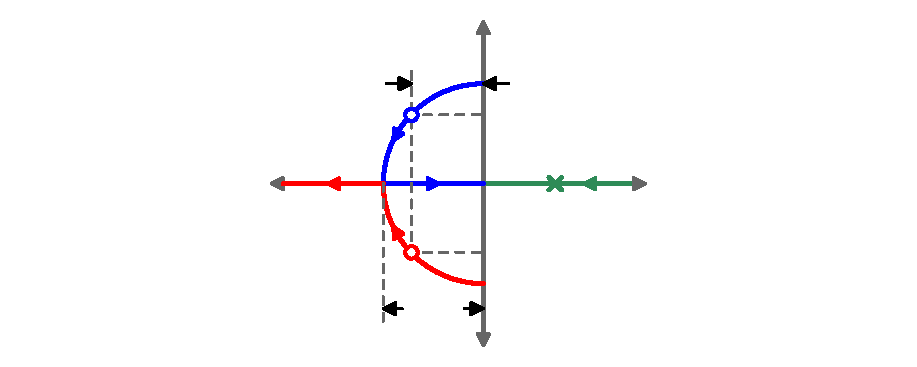
\includegraphics[scale=0.70000]{./figs/pi_pz_plot.pdf}\\
   % translate x=800 y=416 scale 0.38
   \putbox{2.85600in}{0.67900in}{1.20}{$\Re(s)$}%
   \putbox{2.30300in}{1.52600in}{1.20}{$\Im(s)$}%
   \putbox{1.89000in}{0.21700in}{1.20}{$\sqrt{\mathrm{K}}$}%
   \putbox{1.45600in}{1.36500in}{1.20}{$\zeta\sqrt{\mathrm{K}}$}%
   \putbox{2.38700in}{0.95900in}{1.20}{$\sqrt{\mathrm{K}}/2\zeta$}%
   } % close 'parbox'
   } % close 'scalebox'
   \vspace{-\baselineskip} % this is not necessary, but looks better
\fontfamily{\rmdefault}\selectfont

				\caption{PI-controller PLL pole-zero locations.}
				\label{fig:pi_pll_pz}
			\end{figure}
			\FloatBarrier
			To illustrate the effect of the damping coefficient $\zeta$, figure \ref{fig:pi_pll_response} illustrates the example frequency and step responses of a PI-controlled PLL with N=1. Notice excessive peaking and ringing for $\zeta<\sqrt{2}/2$. The peaking observed in the frequency response is unavoidable with the PI-PLL due to the inherent zero in the transfer function. Its effect can be reduced with large $\zeta$, however this will increase PLL settling time. 
			\begin{figure}[htb!]
				\center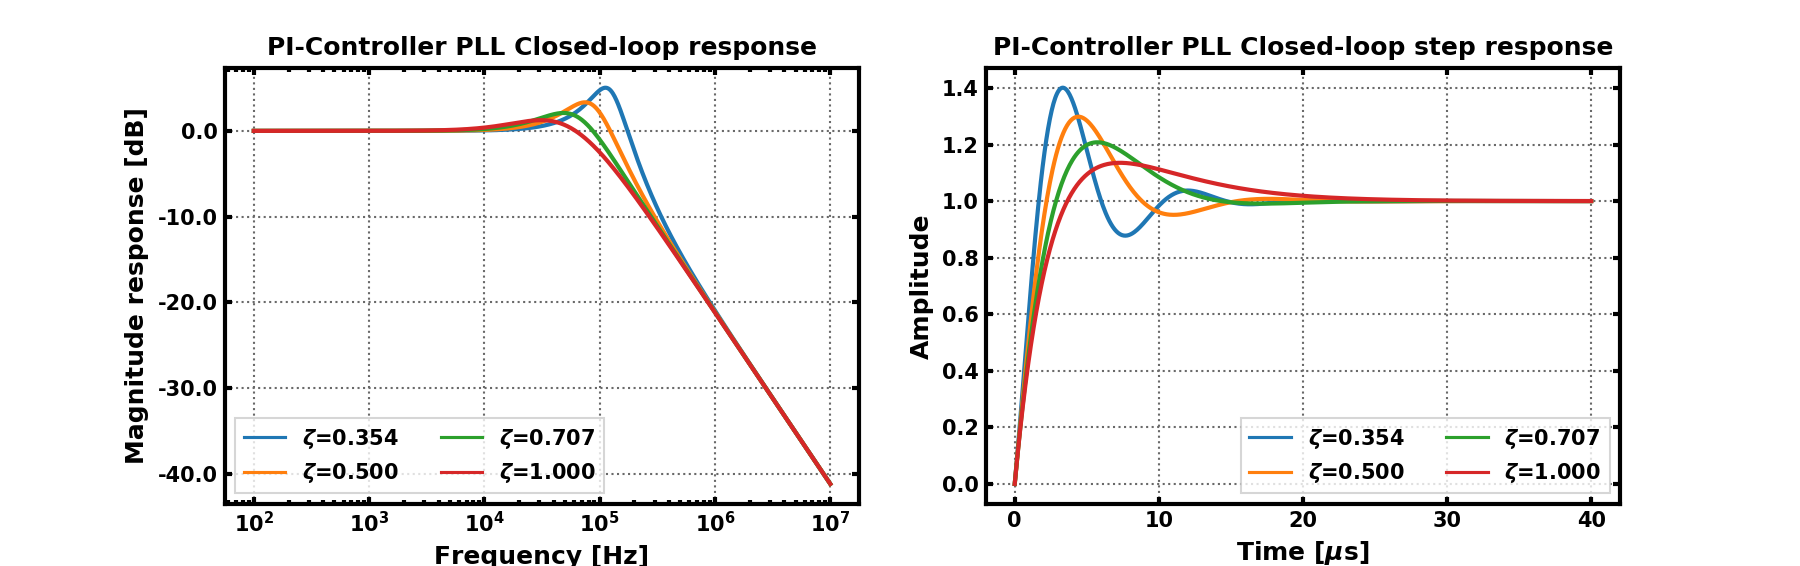
\includegraphics[width=1.0\textwidth, angle=0]{figs/pi_pll_response2.png}
				\caption{Example PI-PLL responses with varied $\zeta$.}
				\label{fig:pi_pll_response}
			\end{figure}
			\FloatBarrier
			If $\zeta$ is constrained to $\leq 1$:
			\begin{equation}
				\tau = \frac{1}{|\min(\Re(\{s_{p1}, s_{p2}\}))|} = \frac{1}{\zeta\sqrt{K}}
			\end{equation}
			Thus:
			\begin{equation}
				t_s = \frac{-\ln(\delta)}{\zeta\sqrt{K}} = \frac{-\ln\left(\frac{f_{tol}}{|f_i - Nf_{ref}|}\right)}{\zeta\sqrt{K}} 
			\end{equation}
			Based on specification for settling time and damping $\zeta$, the values for K and $\omega_z$ can be determined. If $K_{VCO}$ and $\mathrm{N}$ are also specified, the PI gain coefficients can be solved additionally.
			\begin{align}
				\omega_z &= \frac{-\ln(\delta)}{2t_s} =  \frac{-\ln\left(\frac{f_{tol}}{|f_i - Nf_{ref}|}\right)}{2t_s}\\
				K &= \frac{\ln^2(\delta)}{\zeta^2t_s^2} =  \frac{\ln^2\left(\frac{f_{tol}}{|f_i - Nf_{ref}|}\right)}{\zeta^2t_s^2}\\
				K_i & = \frac{\mathrm{N}\mathrm{K}}{2\pi K_{VCO}} \\
				K_p & = \frac{K_i}{\omega_z}
			\end{align}

		\subsubsection{PI-controller peaking compensation}
			 To compensate for closed loop peaking, the original PI-controller loop filter of equation \ref{eq:pi_pll_tf} can be modified with the addition of a single tunable pole at $\omega_p$. The closed loop response becomes third order, which complicates direct analysis and design of the loop filter. However, utilizing the automated filter optimization approach described later in this paper resolved issues regarding filter design in this case.
			\begin{equation} \label{eq:pi_compensated_tf}
				\textnormal{H}_{LF}(s) = \frac{K_i}{s}\frac{\left(\frac{s}{\omega_z} + 1\right)}{\left(\frac{s}{\omega_p} + 1\right)}
			\end{equation}

		\subsubsection{Alternative PID controller permutations} \label{other_pid}
			If individual terms within the PID-controller are dropped, different controller permutations (PD, ID, PI, P, I, D) can be achieved. As mentioned before, inclusion of an integral term is needed to ensure the desired zero steady state error for a PLL. This leaves ID and I-controllers as possible alternative solutions to PI for the loop filter. However, it can be easily found that neither of these controllers result in a stable PLL, which leaves a PI-controller as the only viable PID implementation.

			\textbf{I-only controller}

			Setting the $K_p$ and $K_d$ terms of equation \ref{eq:pid_pll_tf} to zero yields:
			\begin{equation}
				\frac{\Phi_{out}(s)}{\Phi_{ref}(s)} = \frac{2\pi K_{VCO}K_i}{s^2 + \frac{2\pi K_{VCO}}{\mathrm{N}}K_i}
			\end{equation}
			This closed loop transfer function results in a pair of poles at $\pm\sqrt{2\pi K_{VCO}K_i/\mathrm{N}}$. This will never be stable, as it can only be manifested as (1) a pair of poles on the imaginary axis, which is an oscillator, or (2) a real pole in the right-half plane and a real pole in the left-half plane, the former of which is not causally stable.

			\textbf{ID-controller}

			Setting the $K_p$ term of equation \ref{eq:pid_pll_tf} to zero yields:
			\begin{equation}
				\frac{\Phi_{out}(s)}{\Phi_{ref}(s)} = \frac{2\pi K_{VCO}\left(s^2K_d + K_i\right)}{s^2\left(1 + \frac{2\pi K_{VCO}K_d}{\mathrm{N}}\right) + \frac{2\pi K_{VCO}}{\mathrm{N}} K_i}
			\end{equation}
			The poles of this transfer have the same form as the I-only controller, and this PLL-controller configuration is unstable for the same reasons as the I-only controller PLL.
	\subsection{Digital, discretized PLL Model}
Based on the continuous PLL theory, a model for digital, discretized PLLs (i.e. ADPLLs) can be adapted. The general approach here is to utilize the bilinear transformation between continuous s-domain models to the discrete z-domain models. As commonly cited in PLL literature from a seminal paper by Gardner \cite{gardner_1980}, if the sampling frequency $f_s > 10\cdot\textnormal{BW}_{loop}$, where BW$_{loop}$ is the PLL loop bandwidth, the effects of time sampling are easily ignored for purposes of analysis. Thus the design methods established in this paper are predicated on $f_s > 10\cdot\textnormal{BW}_{loop}$.
\begin{figure}[htb!]
	\center\fontfamily{\sfdefault}\selectfont
% XCircuit output "basic_adpll.tex" for LaTeX input from basic_adpll.ps
\def\putbox#1#2#3#4{\makebox[0.00000in][l]{\makebox[#1][l]{}\raisebox{\baselineskip}[0.00000in][0.00000in]{\raisebox{#2}[0.00000in][0.00000in]{\scalebox{#3}{#4}}}}}
\def\rightbox#1{\makebox[0.00000in][r]{#1}}
\def\centbox#1{\makebox[0.00000in]{#1}}
\def\topbox#1{\raisebox{-0.60\baselineskip}[0.00000in][0.00000in]{#1}}
\def\midbox#1{\raisebox{-0.20\baselineskip}[0.00000in][0.00000in]{#1}}
   \scalebox{1}{
   \normalsize
   \parbox{5.07500in}{
   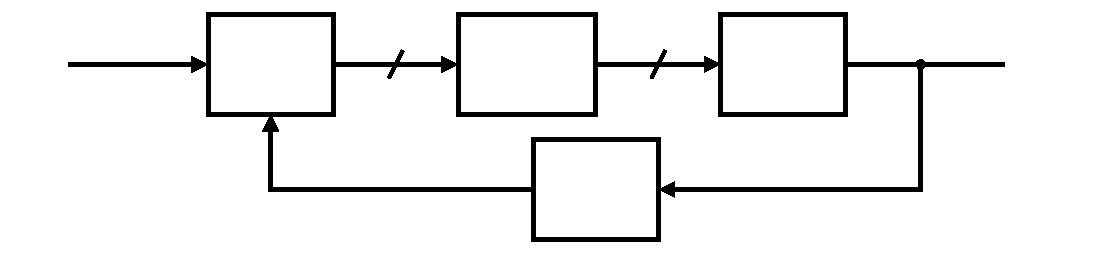
\includegraphics[scale=0.70000]{./figs/basic_adpll.pdf}\\
   % translate x=368 y=488 scale 0.38
   \putbox{1.09200in}{0.82600in}{1.20}{TDC}%
   \putbox{2.63200in}{0.24500in}{1.20}{$\div$ N}%
   \putbox{0.35700in}{0.97300in}{1.20}{$\Phi_{ref}$[n]}%
   \putbox{4.09500in}{0.97300in}{1.20}{$\Phi_{out}$[n]}%
   \putbox{2.19800in}{0.82600in}{1.20}{H$_{LF}$(z)}%
   \putbox{3.47900in}{0.82600in}{1.20}{DCO}%
   \putbox{1.67300in}{0.39200in}{1.20}{$\Phi_{div}$[n]}%
   \putbox{1.64500in}{1.02900in}{1.20}{e$_{\Phi}$[n]}%
   \putbox{2.92600in}{1.02900in}{1.20}{u[n]}%
   } % close 'parbox'
   } % close 'scalebox'
   \vspace{-\baselineskip} % this is not necessary, but looks better
\fontfamily{\rmdefault}\selectfont

	\caption{Basic ADPLL.}
	\label{fig:basic_adpll}
\end{figure}
\FloatBarrier
The basic architecture of an ADPLL is shown in figure \ref{fig:basic_adpll}. Here, compared to the continuous PLL, the phase detector has been replaced with a time to digital converter (TDC), the loop filter $\mathrm{H}_{LF}(s)$ with a discrete loop filter $\mathrm{H}_{LF}(z)$, and the VCO with a digitally controlled oscillator (DCO). In this architecture, the TDC, loop filter, and DCO are digital. 

\subsubsection{Divider}
A digital divider behaves nearly identical to the continuous case:
\begin{equation}
	\Phi_{div}[n] = \frac{\Phi_{out}[n]}{\mathrm{N}}
\end{equation}
Application of the z-transform:
\begin{equation}
	\frac{\Phi_{div}(z)}{\Phi_{out}(z)} = \frac{1}{\mathrm{N}}
\end{equation}
\subsubsection{TDC}
The TDC is a digital, quantized representation of the the phase detector. It takes input phase signals $\Phi_{div}$[n] and $\Phi_{ref}$[n], and outputs a digital phase error measurement word $e_\Phi[n]$. Figure \ref{fig:tdc} shows the basic TDC model architecture. A TDC will have limited resolution in phase, equivalent to M steps per reference cycle. This is a minimum step size in time of $\Delta t_{step}$ = $1/Mf_{ref}$. Since the output of the TDC is digital, the model applies a scale factor M$/2\pi$ and floor rounding, so 1 LSB of $e_\Phi[n]$ equates to $\Delta t_{step}$ timing error  between $\Phi_{div}$[n] and $\Phi_{ref}$[n].
\begin{figure}[htb!]
	\center\fontfamily{\sfdefault}\selectfont
% XCircuit output "tdc.tex" for LaTeX input from tdc.ps
\def\putbox#1#2#3#4{\makebox[0.00000in][l]{\makebox[#1][l]{}\raisebox{\baselineskip}[0.00000in][0.00000in]{\raisebox{#2}[0.00000in][0.00000in]{\scalebox{#3}{#4}}}}}
\def\rightbox#1{\makebox[0.00000in][r]{#1}}
\def\centbox#1{\makebox[0.00000in]{#1}}
\def\topbox#1{\raisebox{-0.60\baselineskip}[0.00000in][0.00000in]{#1}}
\def\midbox#1{\raisebox{-0.20\baselineskip}[0.00000in][0.00000in]{#1}}
   \scalebox{1}{
   \normalsize
   \parbox{3.50000in}{
   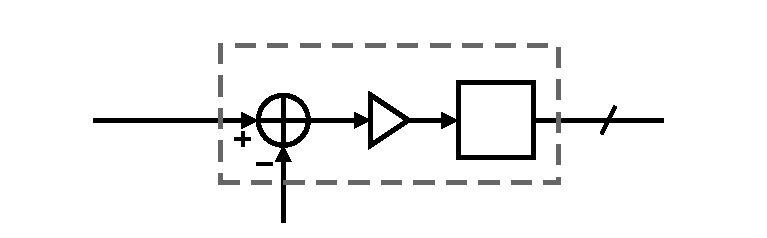
\includegraphics[scale=0.70000]{./figs/tdc.pdf}\\
   % translate x=432 y=396 scale 0.38
   \putbox{0.46200in}{0.63700in}{1.20}{$\Phi_{ref}$[n]}%
   \putbox{1.35100in}{0.08400in}{1.20}{$\Phi_{div}$[n]}%
   \putbox{2.68100in}{0.66500in}{1.20}{e$_\Phi$[n]}%
   \putbox{1.77800in}{0.70700in}{1.20}{\rotatebox{-360}{$\frac{\mathrm{M}}{2\pi}$}}%
   \putbox{1.47000in}{0.63700in}{1.20}{$\Phi_e$}%
   \putbox{2.18400in}{0.50400in}{1.20}{$\lfloor x\rfloor$}%
   \putbox{1.02900in}{0.95900in}{1.20}{TDC}%
   } % close 'parbox'
   } % close 'scalebox'
   \vspace{-\baselineskip} % this is not necessary, but looks better
\fontfamily{\rmdefault}\selectfont

	\caption{TDC model.}
	\label{fig:tdc}
\end{figure}
\begin{equation}
	e_\Phi[n] = \left\lfloor\frac{\mathrm{M}}{2\pi}(\Phi_{ref}[n] - \Phi_{div}[n])\right\rfloor
\end{equation}
For purposes of PLL transfer function calculation, the z-domain representation is as follows. Effects of quantization will be handled in section \ref{pn_theory}.
\begin{equation}
	e_\Phi(z) = \frac{\mathrm{M}}{2\pi}(\Phi_{ref}(z) - \Phi_{div}(z))
\end{equation}	
\FloatBarrier
\subsubsection{Loop Filter}
The loop filter design will be derived from the continuous PI-controller loop filter with optional peaking compensation (equation \ref{eq:pi_compensated_tf}) via application of the bilinear transform. The bilinear transform specifically allows for the conversion of a continuous transfer function to discrete representation, and vice versa. This, however is conditioned on satisfaction of Nyquist sampling criteria, and in the case of PLLs it is recommended that $f_s > 10\cdot\mathrm{BW}_{loop}$ to ensure transformation accuracy \cite{gardner_1980}. A high level of oversampling allows for the following definition of the bilinear transform, where 1/T=$f_{ref}$:
\begin{align*}
	z^{-1} &= e^{-sT} && \text{(definition of z-space)} \\
	&= \sum_{k=0}^\infty\frac{(-sT)^k}{k!} && \text{(exponential Taylor series)} \\
	&\approx 1-sT &&\text{(if $|sT| = 2\pi\mathrm{BW}_{loop}\cdot T << 1$)} \\
\end{align*}
Thus the bilinear transform identities are:
\begin{align}
	z^{-1} &= 1-sT\\
	s &= \frac{1}{T}(1-z^{-1}) \label{eq:s_to_z}
\end{align}
Applying \ref{eq:s_to_z} to equation \ref{eq:pi_compensated_tf} yields the z-domain loop filter:
\begin{align}
	\textnormal{H}_{LF}(z) = \left.\textnormal{H}_{LF}(s)\right\vert_{s=\frac{1}{T}(1-z^{-1})} = \left.\frac{K_i}{s}\frac{\left(\frac{s}{\omega_z} + 1\right)}{\left(\frac{s}{\omega_p} + 1\right)}\right\vert_{s=\frac{1}{T}(1-z^{-1})}\\
	= \frac{\omega_p}{\omega_z}\frac{k_iT}{(1-z^{-1})}\frac{(1+\omega_zT)-z^{-1}}{(1+\omega_pT) - z^{-1}(2+\omega_pT) + z^{-2}}\label{eq:z_lf}
\end{align}
Equation \ref{eq:z_lf} is converted to a digitally implementable representation via converting into the canonical representation of \ref{eq:canonical_z}, which determines the tap coefficients for the sampled-time difference equation \ref{eq:cananical_diff}. 
\begin{align}
	\textnormal{H}_{LF}(z) &= \frac{\sum_{j=0}^M b_jz^{-j}}{1+\sum_{k=1}^N a_kz^{-k}}\label{eq:canonical_z} \\
	y[n]&= -\sum_{k=1}^N a_ky[n-k] + \sum_{j=0}^M b_jx[n-j] \label{eq:cananical_diff}
\end{align}
Equation \ref{eq:cananical_diff} is directly implementable in digital hardware with a direct type 1 IIR filter shown in figure \ref{fig:filt_imple}, with the filter coefficients given by equations \ref{eq:a1}-\ref{eq:b1}. The filter coefficients must be quantized into finite resolution fixed point words for a complete digital implementation. Effects of quantization will be discussed in section \ref{pn_theory}.
\begin{figure}[htb!]
	\center\fontfamily{\sfdefault}\selectfont
% XCircuit output "filter_arch_tex.tex" for LaTeX input from filter_arch_tex.ps
\def\putbox#1#2#3#4{\makebox[0.00000in][l]{\makebox[#1][l]{}\raisebox{\baselineskip}[0.00000in][0.00000in]{\raisebox{#2}[0.00000in][0.00000in]{\scalebox{#3}{#4}}}}}
\def\rightbox#1{\makebox[0.00000in][r]{#1}}
\def\centbox#1{\makebox[0.00000in]{#1}}
\def\topbox#1{\raisebox{-0.60\baselineskip}[0.00000in][0.00000in]{#1}}
\def\midbox#1{\raisebox{-0.20\baselineskip}[0.00000in][0.00000in]{#1}}
   \scalebox{1}{
   \normalsize
   \parbox{5.54167in}{
   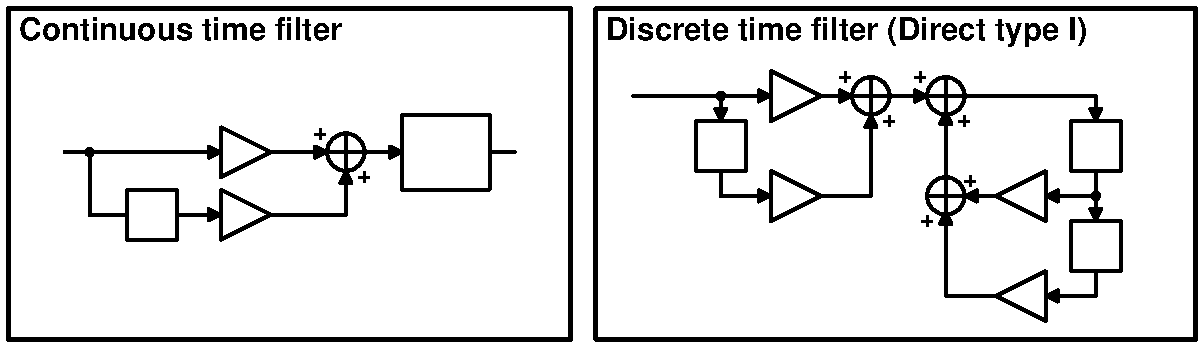
\includegraphics[scale=0.70000]{./figs/filter_arch_tex.pdf}\\
   % translate x=1728 y=944 scale 0.38
   \putbox{1.91800in}{0.90300in}{0.96}{$\frac{1}{\frac{s}{\omega_p} + 1}$}%
   \putbox{1.14800in}{1.01500in}{0.96}{$K_p$}%
   \putbox{1.14800in}{0.72800in}{0.96}{$K_i$}%
   \putbox{0.60900in}{0.58100in}{0.96}{$1/s$}%
   \putbox{0.25900in}{0.98700in}{0.96}{x[n]}%
   \putbox{2.35900in}{0.98700in}{0.96}{y[n]}%
   \putbox{2.92600in}{1.25300in}{0.96}{x[n]}%
   \putbox{5.17300in}{1.16200in}{0.96}{y[n]}%
   \putbox{3.26200in}{0.90300in}{0.96}{$z^{-1}$}%
   \putbox{3.73100in}{1.28100in}{0.96}{b$_0$}%
   \putbox{3.73100in}{0.81200in}{0.96}{b$_1$}%
   \putbox{5.01200in}{0.90300in}{0.96}{$z^{-1}$}%
   \putbox{5.01200in}{0.43400in}{0.96}{$z^{-1}$}%
   \putbox{4.60600in}{0.82600in}{0.96}{-a$_1$}%
   \putbox{4.59200in}{0.35700in}{0.96}{-a$_2$}%
   \putbox{5.17300in}{0.69300in}{0.96}{y[n-1]}%
   \putbox{5.15900in}{0.23100in}{0.96}{y[n-2]}%
   } % close 'parbox'
   } % close 'scalebox'
   \vspace{-\baselineskip} % this is not necessary, but looks better
\fontfamily{\rmdefault}\selectfont

	\caption{Implementation of filter.}
	\label{fig:filt_imple}
\end{figure}
			% y[n] = x[n]\frac{K_i\omega_pT}{\omega_z}\frac{1+\omega_zT}{1+\omega_pT} - x[n-1]\frac{K_i\omega_pT}{\omega_z}\frac{1}{1+\omega_pT} + y[n-1]\frac{2+\omega_pT}{1+\omega_pT} - y[n-2]\frac{1}{1+\omega_pT}\\
			% = a_0x[n] + a_1x[n-1] - b_1y[n-1] - b_2x[n-2] 
\begin{align}
	a_1 &= -\frac{2+\omega_pT}{1+\omega_pT}\label{eq:a1}\\
	a_2 &= \frac{1}{1+\omega_pT} \\
	b_0 &= \frac{K_i\omega_pT}{\omega_z}\frac{1+\omega_zT}{1+\omega_pT}\\
	b_1 &= \frac{K_i\omega_pT}{\omega_z}\frac{1}{1+\omega_pT}\label{eq:b1}
\end{align}
\subsubsection{DCO}
The DCO is modeled in discrete time as a recursive phase integrator, dependent on the DCO gain $K_{DCO}$, which provides the frequency tuning per LSB of the oscillator, the input oscillator tuning word u[n], and the sampling period T.
\begin{equation}
	\Phi_{out}[n] = \Phi_{out}[n-1] + 2\pi K_{DCO}u[n]T
\end{equation}
Application of the z-transform yields:
\begin{equation}
	\frac{\Phi_{out}(z)}{u(z)} = \frac{2\pi K_{DCO}T}{1-z^{-1}}
\end{equation}
Application of the bilinear transform to the DCO transfer function yields:
\begin{equation}
	\frac{\Phi_{out}(s)}{u(s)} = \frac{2\pi K_{DCO}T}{1-(1-sT)} = \frac{2\pi K_{DCO}}{s} 
\end{equation}
\subsubsection{Discrete-time PLL transfer function}
\begin{figure}[htb!]
	\center\fontfamily{\sfdefault}\selectfont
% XCircuit output "discrete_pll.tex" for LaTeX input from discrete_pll.ps
\def\putbox#1#2#3#4{\makebox[0.00000in][l]{\makebox[#1][l]{}\raisebox{\baselineskip}[0.00000in][0.00000in]{\raisebox{#2}[0.00000in][0.00000in]{\scalebox{#3}{#4}}}}}
\def\rightbox#1{\makebox[0.00000in][r]{#1}}
\def\centbox#1{\makebox[0.00000in]{#1}}
\def\topbox#1{\raisebox{-0.60\baselineskip}[0.00000in][0.00000in]{#1}}
\def\midbox#1{\raisebox{-0.20\baselineskip}[0.00000in][0.00000in]{#1}}
   \scalebox{1}{
   \normalsize
   \parbox{6.88333in}{
   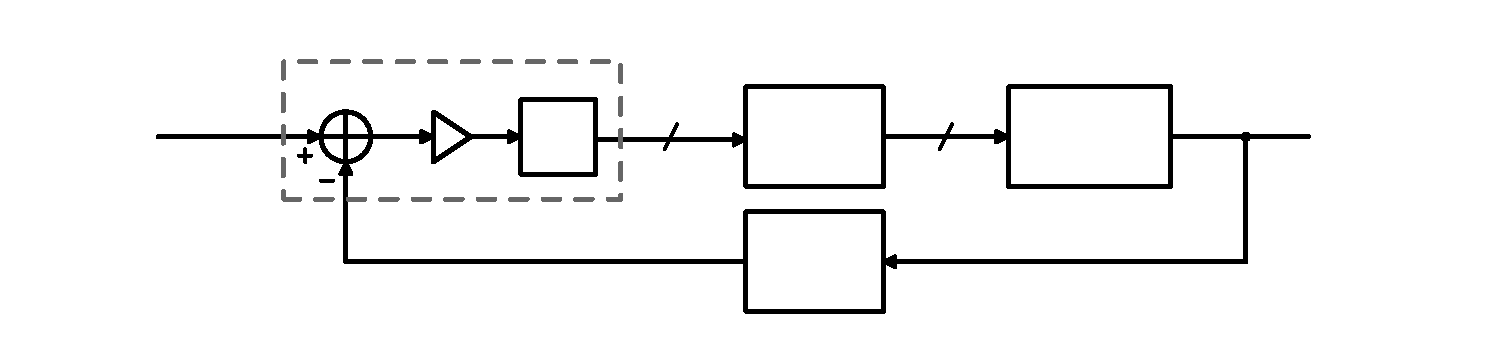
\includegraphics[scale=0.70000]{./figs/discrete_pll.pdf}\\
   % translate x=512 y=508 scale 0.38
   \putbox{0.74200in}{1.04300in}{1.20}{$\Phi_{ref}$[n]}%
   \putbox{2.17000in}{0.47600in}{1.20}{$\Phi_{div}$[n]}%
   \putbox{3.00300in}{1.07800in}{1.20}{e$_\Phi$[n]}%
   \putbox{2.06500in}{1.12000in}{1.20}{\rotatebox{-360}{$\frac{\mathrm{M}}{2\pi}$}}%
   \putbox{1.75700in}{1.04300in}{1.20}{$\Phi_e$}%
   \putbox{2.47800in}{0.91700in}{1.20}{$\lfloor x\rfloor$}%
   \putbox{1.32300in}{1.36500in}{0.90}{TDC}%
   \putbox{3.55600in}{0.91700in}{1.20}{H$_{LF}$(z)}%
   \putbox{4.28400in}{1.07800in}{1.20}{u[n]}%
   \putbox{4.73200in}{0.93100in}{1.20}{$\frac{2\pi K_{DCO}T}{1-z^{-1}}$}%
   \putbox{5.55100in}{1.04300in}{1.20}{$\Phi_{out}$[n]}%
   \putbox{3.62600in}{0.32900in}{1.20}{$\div$ N}%
   \putbox{4.70400in}{1.23200in}{0.90}{DCO}%
   } % close 'parbox'
   } % close 'scalebox'
   \vspace{-\baselineskip} % this is not necessary, but looks better
\fontfamily{\rmdefault}\selectfont

	\caption{Discrete time PLL model.}
	\label{fig:discrete_pll2}
\end{figure}
\FloatBarrier
The transfer function for the discrete-time PLL can be computed in the z-domain, and also approximated continuously. The open loop z-domain transfer function is:
\begin{align}
\mathrm{OL}(z) = \mathrm{H}_{TDC}(z)\mathrm{H}_{LF}(z)\mathrm{H}_{DCO}(z)\mathrm{H}_{DIV}(z) = \\
2\pi K_{DCO}K_iT^2\frac{\mathrm{M}}{\mathrm{N}}\frac{\omega_p}{\omega_z}\frac{(1+\omega_zT)-z^{-1}}{(1+\omega_pT) - z^{-1}(3+2\omega_pT) + z^{-2}(3+\omega_pT) - z^{-3}}\label{eq:z_lf}
\end{align}
The closed loop z-domain PLL phase transfer function is:
\begin{align}
\frac{\Phi_{out}(z)}{\Phi_{ref}(z)} = \frac{\mathrm{H}_{DIV}(z)^{-1}\mathrm{OL}(z)}{1+\mathrm{OL}(z)} = \\
\frac{2\pi K_{DCO}K_iT^2\mathrm{M}\frac{\omega_p}{\omega_z}(1+\omega_zT)-z^{-1}}{(1+\omega_pT + 2\pi K_{DCO}K_iT^2\frac{\mathrm{M}}{\mathrm{N}}\frac{\omega_p}{\omega_z}(1+\omega_zT))- z^{-1}(3+2\omega_pT+2\pi K_{DCO}K_iT^2\frac{\mathrm{M}}{\mathrm{N}}\frac{\omega_p}{\omega_z})+ z^{-2}(3+\omega_pT) - z^{-3}}
\end{align}
The s-domain approximation of the transfer function is:
\begin{align}
\mathrm{OL}(s) = \mathrm{H}_{TDC}(s)\mathrm{H}_{LF}(s)\mathrm{H}_{DCO}(s)\mathrm{H}_{DIV}(s) = \frac{\mathrm{M}}{\mathrm{N}}\frac{K_{DCO}K_i}{s^2} \frac{\left(\frac{s}{\omega_z} + 1\right)}{\left(\frac{s}{\omega_p} + 1\right)}
\end{align}
And in closed loop configuration the PLL phase transfer function is:
\begin{align}
\frac{\Phi_{out}(z)}{\Phi_{ref}(z)} = \frac{\mathrm{H}_{DIV}(z)^{-1}\mathrm{OL}(z)}{1+\mathrm{OL}(z)} = \frac{\mathrm{M}K_{DCO}K_i\left(\frac{s}{\omega_z} + 1\right)}{s^3\frac{1}{\omega_z} + s^2 + \frac{\mathrm{M}}{\mathrm{N}}K_{DCO}K_i\left(\frac{s}{\omega_z} + 1\right)}
\end{align}
Incidentally, the s-domain approximation is significantly simpler and will is preferred in this paper for purposes of analysis.


\subsection{PLL Noise} \label{pn_theory}
The predominant sources of noise in the discrete-time ADPLL are chiefly quantization (in the TDC, loop filter, and DCO), along with thermal noise (in the DCO, divider and TDC). The noise generated by these quantization sources will be discussed in the following sections.

\subsubsection{TDC noise}
The predominant phase noise source in the TDC is due to quantization. A straightforward approach to model quantization noise is to utilize the model of figure \ref{fig:tdc_add_pn} to represent quantization.
\hspace{-20em}\begin{figure}[htb!]
    \centering
    \begin{subfigure}{0.5\textwidth}
        \centering
        \fontfamily{\sfdefault}\selectfont
% XCircuit output "tdc.tex" for LaTeX input from tdc.ps
\def\putbox#1#2#3#4{\makebox[0.00000in][l]{\makebox[#1][l]{}\raisebox{\baselineskip}[0.00000in][0.00000in]{\raisebox{#2}[0.00000in][0.00000in]{\scalebox{#3}{#4}}}}}
\def\rightbox#1{\makebox[0.00000in][r]{#1}}
\def\centbox#1{\makebox[0.00000in]{#1}}
\def\topbox#1{\raisebox{-0.60\baselineskip}[0.00000in][0.00000in]{#1}}
\def\midbox#1{\raisebox{-0.20\baselineskip}[0.00000in][0.00000in]{#1}}
   \scalebox{1}{
   \normalsize
   \parbox{3.50000in}{
   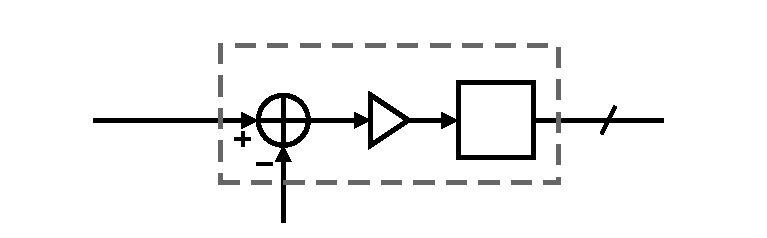
\includegraphics[scale=0.70000]{./figs/tdc.pdf}\\
   % translate x=432 y=396 scale 0.38
   \putbox{0.46200in}{0.63700in}{1.20}{$\Phi_{ref}$[n]}%
   \putbox{1.35100in}{0.08400in}{1.20}{$\Phi_{div}$[n]}%
   \putbox{2.68100in}{0.66500in}{1.20}{e$_\Phi$[n]}%
   \putbox{1.77800in}{0.70700in}{1.20}{\rotatebox{-360}{$\frac{\mathrm{M}}{2\pi}$}}%
   \putbox{1.47000in}{0.63700in}{1.20}{$\Phi_e$}%
   \putbox{2.18400in}{0.50400in}{1.20}{$\lfloor x\rfloor$}%
   \putbox{1.02900in}{0.95900in}{1.20}{TDC}%
   } % close 'parbox'
   } % close 'scalebox'
   \vspace{-\baselineskip} % this is not necessary, but looks better
\fontfamily{\rmdefault}\selectfont

        \caption{TDC Model.}
        \label{fig:tdc1}
    \end{subfigure}%
    \begin{subfigure}{0.5\textwidth}
        \centering
        \fontfamily{\sfdefault}\selectfont
% XCircuit output "tdc_quant.tex" for LaTeX input from tdc_quant.ps
\def\putbox#1#2#3#4{\makebox[0.00000in][l]{\makebox[#1][l]{}\raisebox{\baselineskip}[0.00000in][0.00000in]{\raisebox{#2}[0.00000in][0.00000in]{\scalebox{#3}{#4}}}}}
\def\rightbox#1{\makebox[0.00000in][r]{#1}}
\def\centbox#1{\makebox[0.00000in]{#1}}
\def\topbox#1{\raisebox{-0.60\baselineskip}[0.00000in][0.00000in]{#1}}
\def\midbox#1{\raisebox{-0.20\baselineskip}[0.00000in][0.00000in]{#1}}
   \scalebox{1}{
   \normalsize
   \parbox{3.50000in}{
   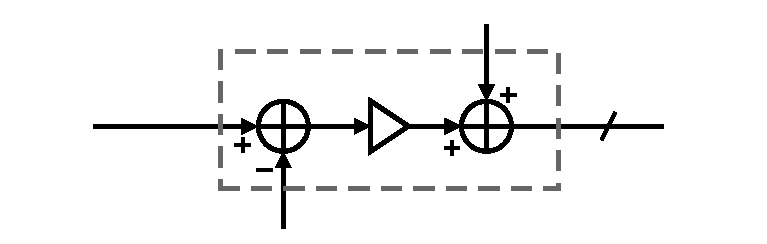
\includegraphics[scale=0.70000]{./figs/tdc_quant.pdf}\\
   % translate x=432 y=396 scale 0.38
   \putbox{0.46200in}{0.63700in}{1.20}{$\Phi_{ref}$[n]}%
   \putbox{1.35100in}{0.08400in}{1.20}{$\Phi_{div}$[n]}%
   \putbox{2.68100in}{0.66500in}{1.20}{e$_\Phi$[n]}%
   \putbox{1.77800in}{0.70700in}{1.20}{\rotatebox{-360}{$\frac{\mathrm{M}}{2\pi}$}}%
   \putbox{1.47000in}{0.63700in}{1.20}{$\Phi_e$}%
   \putbox{2.31700in}{0.97300in}{1.20}{q$_{TDC}$[n]}%
   \putbox{1.02900in}{0.95900in}{1.20}{TDC}%
   } % close 'parbox'
   } % close 'scalebox'
   \vspace{-\baselineskip} % this is not necessary, but looks better
\fontfamily{\rmdefault}\selectfont

        \caption{TDC additive noise model.}
        \label{fig:tdc_add_pn}
    \end{subfigure}
    % \caption{Approximate model for ring oscillator inverter delay cell.}
    \label{fig:tdc_pn_model}
\end{figure}
\FloatBarrier
Using this model, the quantized signal $e_\Phi$[n] is the sum of the its unquantized representation $\Phi_e\frac{\mathrm{M}}{2\pi}$ with a quantization error signal $\mathrm{q}_{TDC}[n]$. Figure \ref{fig:quantization} illustrates this process.
\begin{figure}[htb!]
	\center\fontfamily{\sfdefault}\selectfont
% XCircuit output "quantization.tex" for LaTeX input from quantization.ps
\def\putbox#1#2#3#4{\makebox[0.00000in][l]{\makebox[#1][l]{}\raisebox{\baselineskip}[0.00000in][0.00000in]{\raisebox{#2}[0.00000in][0.00000in]{\scalebox{#3}{#4}}}}}
\def\rightbox#1{\makebox[0.00000in][r]{#1}}
\def\centbox#1{\makebox[0.00000in]{#1}}
\def\topbox#1{\raisebox{-0.60\baselineskip}[0.00000in][0.00000in]{#1}}
\def\midbox#1{\raisebox{-0.20\baselineskip}[0.00000in][0.00000in]{#1}}
   \scalebox{1}{
   \normalsize
   \parbox{4.24010in}{
   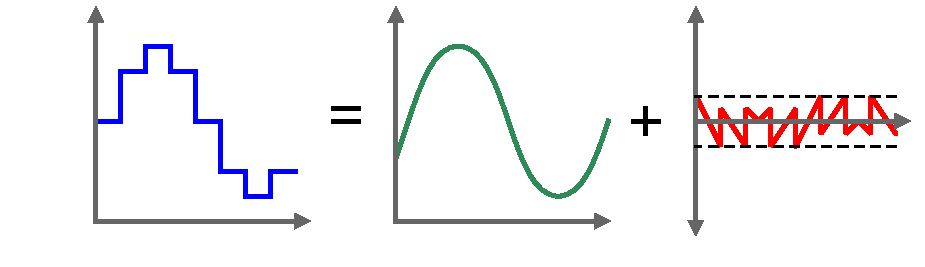
\includegraphics[scale=0.70000]{./figs/quantization.pdf}\\
   % translate x=304 y=240 scale 0.38
   \putbox{0.04200in}{1.09200in}{0.96}{$e_\Phi$[n]}%
   \putbox{1.32300in}{0.04200in}{0.96}{t=nT}%
   \putbox{1.32300in}{1.09200in}{0.96}{$\frac{\mathrm{M}}{2\pi}\Phi_e$[n]}%
   \putbox{2.77900in}{0.04200in}{0.96}{\rotatebox{-360}{t}}%
   \putbox{4.24200in}{0.50400in}{0.96}{t}%
   \putbox{2.72300in}{1.09200in}{0.96}{q$_{\mathrm{TDC}}$[n]}%
   \putbox{3.47900in}{0.85400in}{0.96}{$+\Delta/2$}%
   \putbox{3.47900in}{0.44800in}{0.96}{$-\Delta/2$}%
   } % close 'parbox'
   } % close 'scalebox'
   \vspace{-\baselineskip} % this is not necessary, but looks better
\fontfamily{\rmdefault}\selectfont

	\caption{Quantization as via additive error signal.}
	\label{fig:quantization}
\end{figure}
\FloatBarrier
The quantization noise signal has the statistical property that it is uniformly distributed in the range $[-\Delta/2, \Delta/2]$, i.e. $P_q(Q=q) =\mathrm{U}(-\Delta/2, \Delta/2)$ if $\Delta$ is the quantization step size. The power of the TDC quantization noise signal is:
\begin{equation}\label{eq:tdc_noise}
\sigma_{q_{TDC}}^2 = \int_{-\infty}^\infty q^2P_q(Q=q)dq =  \int_{-\Delta/2}^{\Delta/2}\frac{q^2}{\Delta}dq = \frac{\Delta^2}{12}
\end{equation}
Since $e_\Phi$[n] is digital signal, the minimum step size is $\Delta$=1 LSB. The TDC quantization noise power is therefore $\sigma_{q_{TDC}}^2 = 1/12$ LSB$^2$. The po
If the quantization noise is assumed to be white, and the TDC is sampled at $f_{ref}$, the quantization PSD is:
\begin{equation}
S_{q_{TDC}} = \frac{P_{q_{TDC}}}{\Delta f} = \frac{\sigma_{q_{TDC}}^2}{f_{ref}} = \frac{\Delta^2}{12f_{ref}} = \frac{1}{12f_{ref}} \hspace{1em}\frac{[\text{LSB}]^2}{[\text{Hz}]}
\end{equation}

\subsubsection{DCO noise}
\begin{figure}[htb!]
	\center\fontfamily{\sfdefault}\selectfont
% XCircuit output "dco_noise.tex" for LaTeX input from dco_noise.ps
\def\putbox#1#2#3#4{\makebox[0.00000in][l]{\makebox[#1][l]{}\raisebox{\baselineskip}[0.00000in][0.00000in]{\raisebox{#2}[0.00000in][0.00000in]{\scalebox{#3}{#4}}}}}
\def\rightbox#1{\makebox[0.00000in][r]{#1}}
\def\centbox#1{\makebox[0.00000in]{#1}}
\def\topbox#1{\raisebox{-0.60\baselineskip}[0.00000in][0.00000in]{#1}}
\def\midbox#1{\raisebox{-0.20\baselineskip}[0.00000in][0.00000in]{#1}}
   \scalebox{1}{
   \normalsize
   \parbox{3.56562in}{
   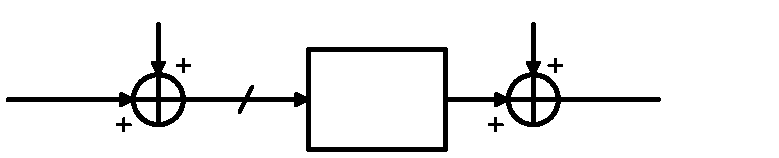
\includegraphics[scale=0.70000]{./figs/dco_noise.pdf}\\
   % translate x=-384 y=320 scale 0.38
   \putbox{1.02900in}{0.39200in}{0.96}{u[n]}%
   \putbox{1.48400in}{0.24500in}{0.96}{$\frac{2\pi K_{DCO}T}{1-z^{-1}}$}%
   \putbox{2.66700in}{0.34300in}{0.96}{$\Phi_{out}$[n]}%
   \putbox{0.78400in}{0.60900in}{0.96}{q$_{OTW}$[n]}%
   \putbox{0.18200in}{0.37800in}{0.96}{$\hat{\textnormal{u}}$[n]}%
   \putbox{2.54800in}{0.62300in}{0.96}{$\Phi_{n_{DCO}}$[n]}%
   } % close 'parbox'
   } % close 'scalebox'
   \vspace{-\baselineskip} % this is not necessary, but looks better
\fontfamily{\rmdefault}\selectfont

	\caption{DCO additive noise model.}
	\label{fig:quantization}
\end{figure}
\FloatBarrier
Noise in the DCO is from quantization of the oscillator tuning word (OTW), and from thermal and stochastic sources. In the digital PLL, the OTW is quantized in loop filter, so this source of noise will be analyzed in the loop filter section. Thus oscillator thermal noise will be considered.
\begin{figure}[htb!]
	\center\fontfamily{\sfdefault}\selectfont
% XCircuit output "aperture_noise.tex" for LaTeX input from aperture_noise.ps
\def\putbox#1#2#3#4{\makebox[0.00000in][l]{\makebox[#1][l]{}\raisebox{\baselineskip}[0.00000in][0.00000in]{\raisebox{#2}[0.00000in][0.00000in]{\scalebox{#3}{#4}}}}}
\def\rightbox#1{\makebox[0.00000in][r]{#1}}
\def\centbox#1{\makebox[0.00000in]{#1}}
\def\topbox#1{\raisebox{-0.60\baselineskip}[0.00000in][0.00000in]{#1}}
\def\midbox#1{\raisebox{-0.20\baselineskip}[0.00000in][0.00000in]{#1}}
   \scalebox{1}{
   \normalsize
   \parbox{2.24062in}{
   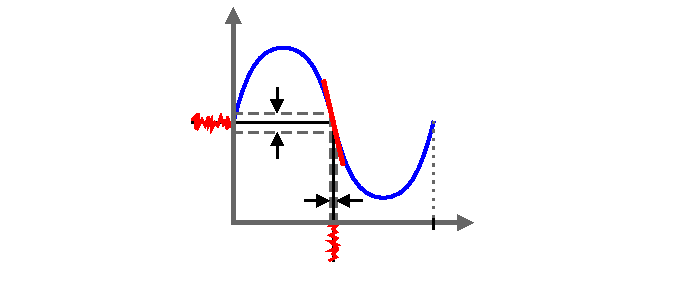
\includegraphics[scale=0.90000]{./figs/aperture_noise.pdf}\\
   % translate x=-108 y=240 scale 0.38
   \putbox{1.87200in}{0.16200in}{0.96}{\rotatebox{-360}{$\Phi$}}%
   \putbox{0.07200in}{1.40400in}{0.96}{V$_{out}$}%
   \putbox{0.63000in}{1.13400in}{0.96}{$\sigma_{v_n}$}%
   \putbox{0.61200in}{0.40500in}{0.96}{$\sigma_{\Phi_n}$}%
   \putbox{0.05400in}{1.06200in}{0.60}{Thermal }%
   \putbox{0.12600in}{0.97200in}{0.60}{noise}%
   \putbox{0.71100in}{0.14400in}{0.60}{Phase }%
   \putbox{0.72900in}{0.05400in}{0.60}{noise}%
   \putbox{1.58400in}{0.14400in}{0.60}{\rotatebox{-360}{$2\pi$}}%
   \putbox{0.40500in}{0.14400in}{0.60}{$0$}%
   } % close 'parbox'
   } % close 'scalebox'
   \vspace{-\baselineskip} % this is not necessary, but looks better
\fontfamily{\rmdefault}\selectfont

	\caption{Thermal to phase noise conversion.}
	\label{fig:quantization}
\end{figure}
\FloatBarrier
 Noise from circuit and supply noise can be realized as an additive voltage component to the oscillator waveform $V_{osc}(t)$, with variance $\sigma_{V_n}^2$. As $V_{osc}(t)$ will have a finite derivative, a small additive noise signal $v_{n}(t)$ will be coupled into the time domain as a phase noise disturbance $\delta\Phi_{n}$ in the oscillator phase. At any point in time, assuming Gaussian white noise, $\delta\Phi_{n}$ is sampled from the following distribution:
 \begin{equation}
 \delta\Phi_{n} \sim \left.\text{Norm}\left(\mu=0, \sigma=\left(\frac{dV(\Phi)}{d\Phi}\right)^{-1}\sigma_{v_n}\right)\right\vert_{\Phi=\omega_{osc}t}
 \end{equation} 
The phase disturbance $\delta\Phi_{n}(t)$ at t is independent of all other points in time. If the phase of the oscillator is analyzed with discrete step $T$:
\begin{equation}
\Phi_{out}[n] = \Phi_{out}[n-1] + \omega_{osc}T + \delta\Phi_n[\Phi=n\omega_{osc} T]
\end{equation}
The contribution only due to phase disturbance, i.e. phase noise $\Phi_n$[n]:
\begin{equation}
\Phi_{n}[n] = \Phi_{out}[n] - \omega_{osc}T = \Phi_{out}[n-1] + \delta\Phi_n[n|\Phi=n\omega_{osc}T]
\end{equation}
Notice this takes the form of a random walk signal. Computing the z-transform
\begin{equation}
\Phi_{n}(z) = \frac{\delta\Phi_n(z)}{1-z^{-1}}
\end{equation}
Application of the bilinear transform can be used to approximate the continuous noise spectrum:
\begin{equation}
\left.\Phi_{n}(z)\right\vert_{z=1-sT} = \left.\frac{\delta\Phi_n(z)}{1-z^{-1}}\right\vert_{z=1-sT} = \frac{\delta\Phi_n(z=1-sT)}{sT}
\end{equation}
The phase noise PSD is therefore:
\begin{equation}
S_{\Phi n_{DCO}}(\omega)= \left|\frac{\delta\Phi_n(z=1-j\omega T)}{j\omega T}\right|^2 = \frac{1}{\omega^2}\left|\frac{\delta\Phi_n(z=1-j\omega T)}{T}\right|^2
\end{equation}
Following that the phase disturbance signal $\delta\Phi_{n}(t)$ is white spectrum, a value for its power $S_{0\Phi n_{DCO}}$ can be defined as such:
\begin{equation}
S_{0\Phi n_{DCO}} = \lim_{T\to0} \mathrm{Var}\left( \left|\frac{\delta\Phi_n(z=1-j\omega T)}{T}\right|^2 \right)
\end{equation}
The value for $S_{0\Phi n_{DCO}}$ is highly dependent on implementation and is best extracted via simulation or physical measurement by fitting the following:
\begin{equation}
S_{\Phi n_{DCO}}(\omega)= \frac{S_{0\Phi n_{DCO}}}{\omega^2}
\end{equation}
\subsubsection{Divider noise}
Divider noise is manifested as jitter on the the output signal, due to thermal noise coupling from voltage to phase. If the divider is a digital circuit, with edge rate $dV/dt$, and subject to thermal noise in the form of a  voltage $v_n$, with noise power of $\sigma_{v_n}^2$, the phase noise (jitter) conferred is:
\begin{equation}
\sigma_{\Phi n_{DIV}} = \omega_{ref}\sigma_{t n_{DIV}}  =\omega_{ref}\left(\frac{dV}{dt}\right)^{-1}\sigma_{v_n}
\end{equation}
Thus the power is:
\begin{equation}
S_{\Phi n_{DIV}} = \omega^2_{ref}\sigma^2_{t n_{DIV}}  =\omega^2_{ref}\left(\frac{dV}{dt}\right)^{-2}\sigma_{v_n}^2
\end{equation}

\subsubsection{Loop filter noise}
Loop filter noise is principally from quantization in the digital case. In the digital loop filter, the mathematical operations are carried out with finite precision, and thus rounding errors occur. Here, an architecture with B bits in each fixed point word throughout the loop filter is assumed for analysis. 

\subsubsection{PLL output-referred noise}\label{pn_noise_psd}
In terms of analysis, PLL noise referred to the PLL output is of most interest. In this case, the noise is defined in terms of phase noise $\Phi_{n}$, or an unwanted added component to the oscillator phase signal $\Phi_{osc}=\omega_{osc}t$. The PLL output phase signal $\Phi_{out}$ is therefore:
\begin{equation}
	\Phi_{out}(t) = \Phi_{osc}(t) + \Phi_{n}(t) = \omega_{osc}t + \Phi_{n}(t) 
\end{equation}
In analyzing phase noise, the noise power spectral density of the PLL output is of most interest. To compute this, an output voltage waveform of the PLL must defined. Given an amplitude $A_0$:
\begin{equation}
V_{out} = \Re\left(A_0e^{j\Phi_{out}(t)}\right) = \Re\left(A_0e^{j\omega_{osc}t}e^{j\Phi_{n}(t)}\right)
\end{equation}
Assuming the phase noise signal is zero mean, $\mathbb{E}[\Phi_{n}(t)]=0$, and the power of phase noise signal is small, $\mathrm{Var}[\Phi_{n}(t)] << 1$, then the approximation $e^{j\Phi_{n}(t)} = 1 + j\Phi_{n}(t)$ can be applied.
\begin{align}
V_{out} = \Re\left(A_0e^{j\omega_{osc}t}e^{j\Phi_{n}(t)}\right) = \Re\left(A_0e^{j\omega_{osc}t} +j\Phi_{n}(t)A_0e^{j\omega_{osc}t}\right)\\
= A_0\cos(\omega_{osc}t) - \Phi_{n}(t)A_0\sin(\omega_{osc}t)
\end{align}
The result is a carrier cosine signal, and an orthogonal sine signal modulated by the phase noise $\Phi_{n}$. From this, the spectral density of the phase noise relative to the carrier can be estimated. Power spectral density is computed as such, assuming the carrier and the phase noise signal components are uncorrelated:
\begin{equation}
S_{V_{out}} = |\mathcal{F}\{V_{out}(t)\}|^2 = A_0^2|\mathcal{F}\{\cos(\omega_{osc}t)\}|^2 + A_0^2|\Phi_{n}(\omega)*\mathcal{F}\{\sin(\omega_{osc}t)\}|^2
\end{equation}
If single side band (SSB) noise power spectral density $\mathcal{L}(\Delta f)$ is defined as the phase noise PSD at offset $\Delta f$ from the carrier frequency $f_{osc}$, normalized to the carrier power:
\begin{equation}
\mathcal{L}(\Delta f) = |\Phi_{n}(2\pi\Delta f)|^2 = |\mathcal{F}\{\Phi_{n}(t)\}|^2= S_{\Phi_{n}}(\Delta f)
\end{equation}
Thus, the PLL output PSD noise relative to the carrier can be computed as the PSD of the phase noise signal $\Phi_{n}(t)$.

\subsubsection{PLL noise sensitivity transfer functions}
Having models for noise of generated by each PLL component, noise sensitivity transfer functions must be computer to refer each noise source to the PLL output in terms of phase. After which, the output noise PSD can be inferred based on the output phase signal, following the theory of section \ref{pn_noise_psd}. An important assumption is made, in that every noise source within the PLL is independent, so that their individual noise powers can be summed at the PLL output to compute the overall PLL output noise.

 and a method to calculate noise power spectral density from the output phase signal


All noise uncorrelated.

Plot of BW vs 
fasf
Generic theory of PLL
Discrete PLL
Noise theory


	% \section{Methods}\label{methods}
	\pagebreak
	% The methods for implementation of a behavioral, discrete-time PLL simulator and for the PLL loop filter automation and optimization will be covered here.

% \hl{Talk about how simulator is implemented:}
% \hl{Discrete simulation models of phase noise, dco etc}
% \hl{Filter optimization}
% \hl{-phase noise and lock time estimate in frequency domain}


\section{Loop Filter Design Automation}\label{methods_lf_design_approach}
The automation approach for ADPLL loop filter design implemented in this work will be outlined here.

\subsection{Design sequence}
	Design automation for ADPLL loop filter is implemented with a strategy that is illustrated in figure \ref{fig:filt_design_seq}, that utilizes a continuous time-approximation based model of the PLL to generate a loop filter design which minimizes the total integrated phase noise power out of the PLL. The optimized continuous filter then undergoes discrete time conversion and mapping into digital representation of the design. Second order optimization is then applied to the discretized and digitized filter implementation, to minimize the effects of quantization error and filter design error due to finite word effects. A discrete-time, behavioral PLL simulator is then used to verify the filter design for proper lock-time, phase noise and stability. The following sections will detail these processes.

	\begin{figure}[htb!]
		\center\fontfamily{\sfdefault}\selectfont
% XCircuit output "filt_design.tex" for LaTeX input from filt_design.ps
\def\putbox#1#2#3#4{\makebox[0.00000in][l]{\makebox[#1][l]{}\raisebox{\baselineskip}[0.00000in][0.00000in]{\raisebox{#2}[0.00000in][0.00000in]{\scalebox{#3}{#4}}}}}
\def\rightbox#1{\makebox[0.00000in][r]{#1}}
\def\centbox#1{\makebox[0.00000in]{#1}}
\def\topbox#1{\raisebox{-0.60\baselineskip}[0.00000in][0.00000in]{#1}}
\def\midbox#1{\raisebox{-0.20\baselineskip}[0.00000in][0.00000in]{#1}}
   \scalebox{1}{
   \normalsize
   \parbox{6.30000in}{
   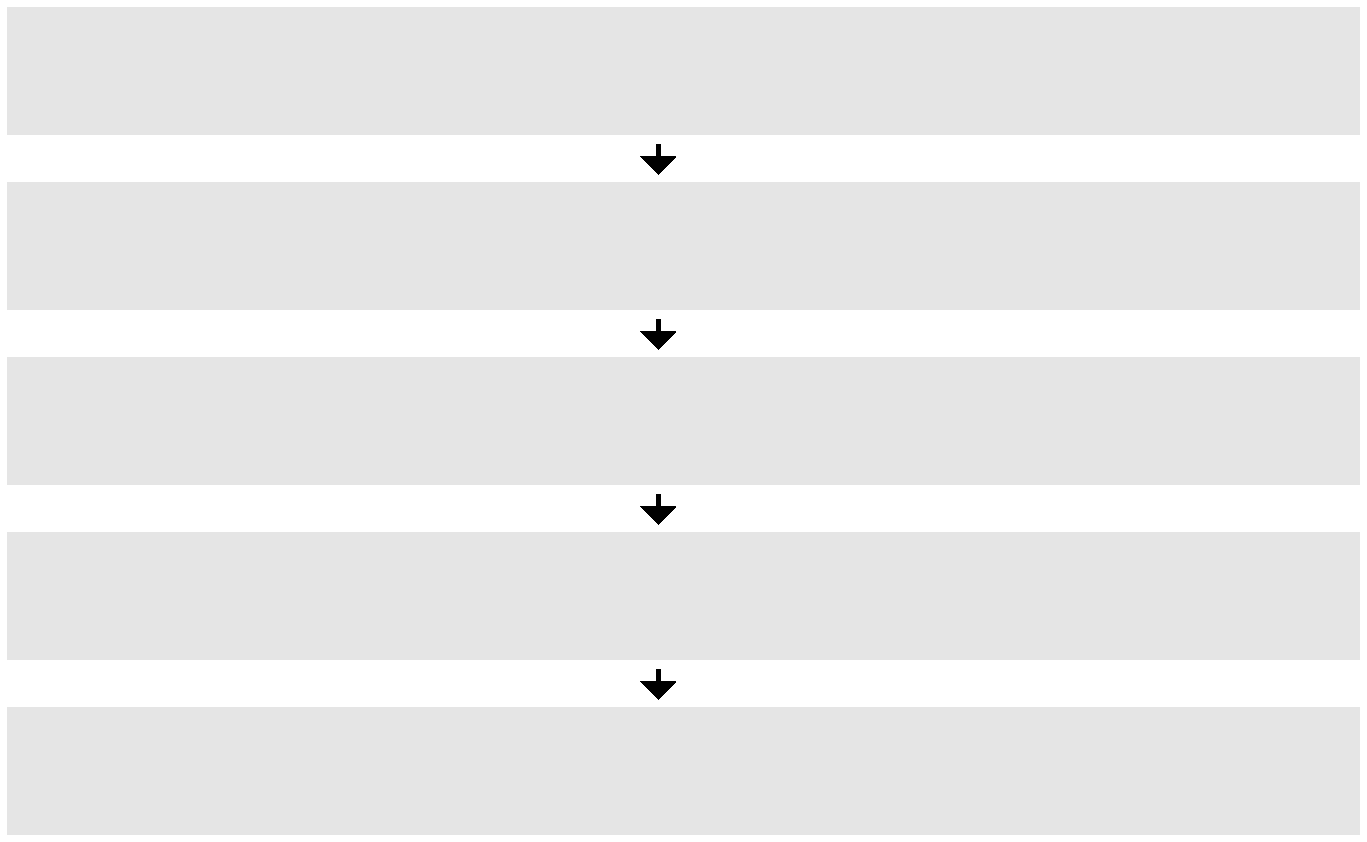
\includegraphics[scale=0.70000]{./figs/filt_design.pdf}\\
   % translate x=192 y=896 scale 0.38
   \putbox{1.90400in}{2.66700in}{0.96}{$T_{opt}(s)=\underset{T(s)}{\argmin}\int_0^{f_h}\mathcal{L}(\Delta f|T(s))d\Delta f$}%
   \putbox{0.09800in}{2.89800in}{0.96}{\textbf{Optimize continuous PLL closed loop response $T(s)$ for minimum total integrated phase noise.}}%
   \putbox{0.09800in}{3.71700in}{0.96}{\textbf{Specify PLL system parameters.}}%
   \putbox{0.18200in}{3.39500in}{0.84}{Divider ratio}%
   \putbox{1.52600in}{3.54200in}{0.84}{TDC resolution}%
   \putbox{1.55400in}{3.39500in}{0.84}{KDCO}%
   \putbox{0.18200in}{3.54200in}{0.84}{Reference frequency}%
   \putbox{3.57000in}{3.54200in}{0.96}{$S_{\Phi n_{DCO}}(f)$}%
   \putbox{0.12600in}{2.07900in}{0.96}{\textbf{Convert $T_{opt}(s)$ into discretized loop filter design.}}%
   \putbox{0.21700in}{1.90400in}{0.84}{Convert $T_{opt}(s)$ to loop filter $H_{LF}(s)$ based on provided system specifications.}%
   \putbox{0.21700in}{1.75700in}{0.84}{Use s-to-z transformation to convert $H_{LF}(s)$ to the discrete time $H_{LF}(z)$.}%
   \putbox{0.12600in}{1.26700in}{0.96}{\textbf{Second order optimize loop filter digital implementation.}}%
   \putbox{0.21700in}{1.09200in}{0.84}{Convert $H_{LF}(z)$ to direct form I implementation of its difference equation.}%
   \putbox{0.21700in}{0.94500in}{0.84}{Optimize number of bits per word used in digital implementation for quantization noise and filter accuracy.}%
   \putbox{0.12600in}{0.44800in}{0.96}{\textbf{Verify design with simulation.}}%
   \putbox{0.21700in}{0.27300in}{0.84}{Utilize behavioral, discrete event simulator to capture non-linear and discrete time effects.}%
   \putbox{0.21700in}{0.12600in}{0.84}{Monte-Carlo sampling for KDCO. initial frequency error to analyze stability, phase noise and lock time across PVT.}%
   \putbox{2.57600in}{3.54200in}{0.84}{DCO phase noise - }%
   } % close 'parbox'
   } % close 'scalebox'
   \vspace{-\baselineskip} % this is not necessary, but looks better
\fontfamily{\rmdefault}\selectfont

		\caption{Filter design sequence.}
		\label{fig:filt_design_seq}
	\end{figure}
	\FloatBarrier

\subsection{Loop filter Prototype}
	The design automation approach developed utilizes a fixed loop filter as a prototype for all loop filter designs. This choice was derived from several criteria that were established for desirable ADPLL operation:
	\begin{enumerate}[itemsep=0pt,label=\protect\mycirc{\arabic*}]
		\setlength\itemsep{-0.8em}
		\item Zero steady state phase error, to ensure accuracy of synthesized frequency.
		\item Loop filter output should remain constant if input (phase error) goes to 0.
		\item Minimize complexity of implemented logic, i.e. minimize the number of poles and zeros.
		\item Low pass response of PLL in closed-loop.
	\end{enumerate}
	To satisfy criterion 1, the loop filter response must include an integrator (1/s) term in the transfer function \cite{ogata_2010}. A PLL with loop filter containing such an integrator is commonly classified as type II, and sans the integrator is type I \cite{gardner_2005}. A rational starting point is to consider a proportional-integral-derivative (PID) controller \cite{ogata_2010_pid} for the loop filter, whose transfer function is given in equation \ref{eq:pid_controller}. This filter contains coefficients $K_d$, $K_p$, $K_i$ which set the gain of the derivative (s), proportional and integral (1/s) terms respectively. 
	\begin{equation}\label{eq:pid_controller}
		\textnormal{H}_{LF}(s) = sK_d + K_p + \frac{K_i}{s} = \frac{K_d}{s}\left(s^2 + s\frac{K_p}{K_d} + \frac{K_i}{K_d}\right)
	\end{equation}
	Application of the loop filter to the continuous ADPLL transfer function model from section \ref{discrete_pll_tf} produces the PLL loop gain in \ref{pid_pll_loop_gain} and the closed loop ADPLL response in \ref{eq:pid_pll_tf}.
	\begin{equation} \label{pid_pll_loop_gain}
		\mathrm{L}(s) = \textnormal{H}_{TDC}(s)\textnormal{H}_{LF}(s)\textnormal{H}_{DCO}(s)\textnormal{H}_{DIV}(s) = \frac{\mathrm{M}}{\mathrm{N}}\frac{K_{DCO}K_d}{s^2}\left(s^2 + s\frac{K_p}{K_d} + \frac{K_i}{K_d}\right)
	\end{equation}
	\begin{align} \label{eq:pid_pll_tf}
		\mathrm{T}(s) = \frac{\Phi_{out}(s)}{\Phi_{ref}(s)} = \frac{\mathrm{M}K_{DCO}K_{d}\left(s^2K_d + sK_p + K_i\right)}{s^2\left(1 + \frac{\mathrm{M}}{\mathrm{N}}K_{DCO}K_d\right) + \frac{\mathrm{M}}{\mathrm{N}}K_{DCO}K_d\left(sK_p + K_i\right)} = \mathrm{N}\frac{\mathrm{L}(s)}{1 + \mathrm{L}(s)}
	\end{align}
	It should be noted that in the closed loop configuration, this PLL phase transfer function contains two poles and two zeros. This is not a low pass response as desired per criterion 4, needed for satisfactory PLL phase noise power spectrum as will later be discussed. In order achieve low pass operation, the derivative term $K_d$ must be set to zero, yielding a proportional-integral (PI) controller for the loop filter:
	\begin{align} \label{eq:full_pi_pll_tf}
		\mathrm{T}(s) = \frac{\Phi_{out}(s)}{\Phi_{ref}(s)} = \frac{\mathrm{M}K_{DCO}\left(sK_p + K_i\right)}{s^2 + \frac{\mathrm{M}}{\mathrm{N}}K_{DCO}\left(sK_p + K_i\right)} = \mathrm{N}\frac{\mathrm{L}(s)}{1 + \mathrm{L}(s)} 
	\end{align}
	Steady state zero phase error can be verified by solving the closed loop $\Phi_e(s)$ for s=0:
	\begin{align}
		\left.\Phi_e(s)\right\vert_{s=0} = \left(\Phi_{ref}(0) - \frac{\Phi_{out}(0)}{\mathrm{N}}\right) = \Phi_{ref}(0)\left(1 - \frac{\Phi_{out}(0)}{\mathrm{N}\Phi_{ref}(0)}\right)= \Phi_{ref}(0)\left(1 - \frac{\mathrm{N}}{\mathrm{N}}\right) = 0
	\end{align}

		\subsubsection{Continuous PI-loop filter design}\label{cont_pi_filt_des}
			Given a PI-controller loop filter, which can be optionally represented using a pole at zero and a zero with $\omega_z = K_i/K_p$:
			\begin{equation} \label{eq:pi_pll_tf}
				\textnormal{H}_{LF}(s) = K_p + \frac{K_i}{s}  = \frac{K_i}{s}\left(\frac{s}{\omega_z} + 1\right) 
			\end{equation}
			Selection of (not-necessarily optimal) PI controller gains can be easily derived from overall PLL settling time requirements. Suppose that settling time $t_s$ is defined such that the PLL settles within $\pm \delta$ of the final value for a step input. If the initial and final PLL output frequencies are $f_i$ and $Nf_{ref}$, and settling with $\pm f_{tol}$ is desired,  $\delta = f_{tol}/|f_i - Nf_{ref}|$. Setting time is therefore:
			\begin{equation}
				t_s = -\tau\ln(\delta)
			\end{equation}
			Thus, to find settling time, a value for the PLL time constant $\tau$ must be derived. Rewriting equation \ref{eq:full_pi_pll_tf} with substitutions $\omega_z = K_i/K_p$ and $\mathrm{K} = MK_{DCO}K_i/\mathrm{N}$:
			\begin{equation} \label{eq:simp_pi_pll_tf}
				\frac{\Phi_{out}(s)}{\Phi_{ref}(s)} = \mathrm{N}\cdot\frac{s\frac{K}{\omega_z} + K }{s^2 + s\frac{K}{\omega_z} + K}
			\end{equation}
			If the second order denominator can be redefined in terms of a natural frequency $\omega_n$ and damping $\zeta$, such that:
			\begin{equation}
				s^2 + s\frac{K}{\omega_z} + K = s^2 + s2\zeta\omega_n + \omega_n^2
			\end{equation}
			It is then found that $\omega_n = \sqrt{K}$, and $\omega_z = \sqrt{K}/2\zeta$. The poles of equation \ref{eq:simp_pi_pll_tf} are then located at s = $\zeta\sqrt{K} \pm \sqrt{K}\sqrt{1-\zeta^2}$.
			The settling time of the PLL will be determined by the real portion of dominant pole of equation \ref{eq:simp_pi_pll_tf}, specifically $\tau = 1/|\min(\Re(\{s_{p1}, s_{p2}\}))|$. Based on the pole-zero plot of figure \ref{fig:pi_pll_pz}, it can be observed that the dominant pole location is maximized with $\zeta=1$. The pole-zero loci orientations are based on increasing $\zeta$ values. According to Razavi \cite{razavi_2017}, $\zeta$ is usually 
			"chosen to be $>\sqrt{2}/2$ or even 1 to avoid excessive ringing."
			\begin{figure}[htb!]
				\center\fontfamily{\sfdefault}\selectfont
% XCircuit output "pi_pz_plot.tex" for LaTeX input from pi_pz_plot.ps
\def\putbox#1#2#3#4{\makebox[0.00000in][l]{\makebox[#1][l]{}\raisebox{\baselineskip}[0.00000in][0.00000in]{\raisebox{#2}[0.00000in][0.00000in]{\scalebox{#3}{#4}}}}}
\def\rightbox#1{\makebox[0.00000in][r]{#1}}
\def\centbox#1{\makebox[0.00000in]{#1}}
\def\topbox#1{\raisebox{-0.60\baselineskip}[0.00000in][0.00000in]{#1}}
\def\midbox#1{\raisebox{-0.20\baselineskip}[0.00000in][0.00000in]{#1}}
   \scalebox{1}{
   \normalsize
   \parbox{4.20000in}{
   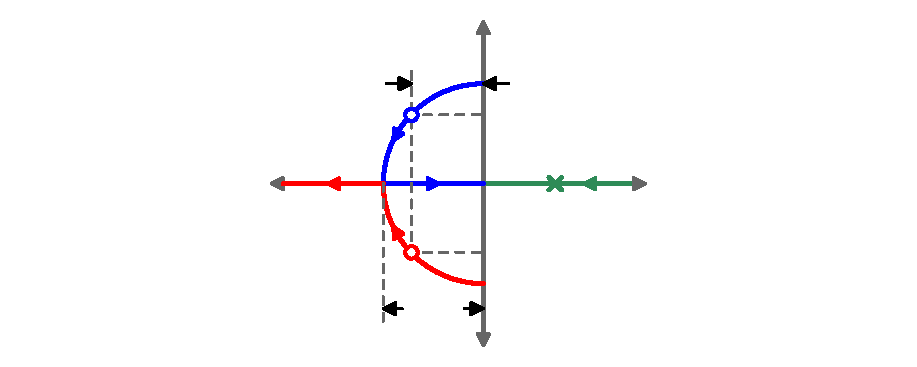
\includegraphics[scale=0.70000]{./figs/pi_pz_plot.pdf}\\
   % translate x=800 y=416 scale 0.38
   \putbox{2.85600in}{0.67900in}{1.20}{$\Re(s)$}%
   \putbox{2.30300in}{1.52600in}{1.20}{$\Im(s)$}%
   \putbox{1.89000in}{0.21700in}{1.20}{$\sqrt{\mathrm{K}}$}%
   \putbox{1.45600in}{1.36500in}{1.20}{$\zeta\sqrt{\mathrm{K}}$}%
   \putbox{2.38700in}{0.95900in}{1.20}{$\sqrt{\mathrm{K}}/2\zeta$}%
   } % close 'parbox'
   } % close 'scalebox'
   \vspace{-\baselineskip} % this is not necessary, but looks better
\fontfamily{\rmdefault}\selectfont

				\caption{PI-controller PLL pole-zero locations.}
				\label{fig:pi_pll_pz}
			\end{figure}
			\FloatBarrier
			To illustrate the effect of the damping coefficient $\zeta$, figure \ref{fig:pi_pll_response} illustrates the example frequency and step responses of a PI-controlled PLL with N=1. Notice excessive peaking and ringing for $\zeta<\sqrt{2}/2$. The peaking observed in the frequency response is unavoidable with the PI-PLL due to the inherent zero in the transfer function. Its effect can be reduced with large $\zeta$, however this will increase PLL settling time. 
			\begin{figure}[htb!]
				\center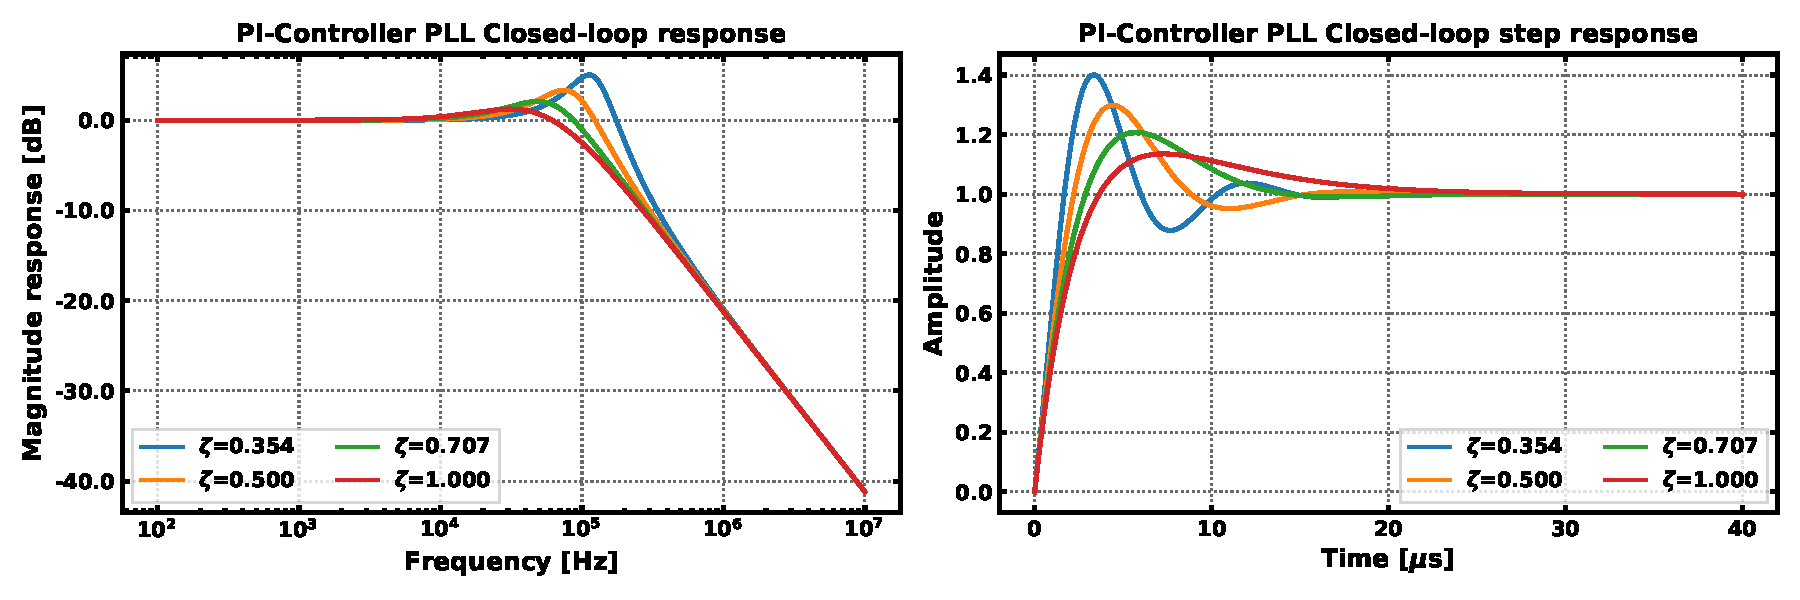
\includegraphics[width=1.0\textwidth, angle=0]{figs/pi_pll_response.pdf}
				\caption{Example PI-PLL responses with varied $\zeta$.}
				\label{fig:pi_pll_response}
			\end{figure}
			\FloatBarrier
			If $\zeta$ is constrained to $\leq 1$:
			\begin{equation}
				\tau = \frac{1}{|\min(\Re(\{s_{p1}, s_{p2}\}))|} = \frac{1}{\zeta\sqrt{K}}
			\end{equation}
			Thus:
			\begin{equation}
				t_s = \frac{-\ln(\delta)}{\zeta\sqrt{K}} = \frac{-\ln\left(\frac{f_{tol}}{|f_i - Nf_{ref}|}\right)}{\zeta\sqrt{K}} 
			\end{equation}
			Based on specification for settling time and damping $\zeta$, the values for K and $\omega_z$ can be determined. If $K_{VCO}$ and $\mathrm{N}$ are also specified, the PI gain coefficients can be solved additionally.
			\begin{align}
				\omega_z &= \frac{-\ln(\delta)}{2t_s} =  \frac{-\ln\left(\frac{f_{tol}}{|f_i - Nf_{ref}|}\right)}{2t_s}\\
				K &= \frac{\ln^2(\delta)}{\zeta^2t_s^2} =  \frac{\ln^2\left(\frac{f_{tol}}{|f_i - Nf_{ref}|}\right)}{\zeta^2t_s^2}\\
				K_i & = \frac{\mathrm{N}}{\mathrm{M}}\frac{\mathrm{K}}{K_{DCO}} \\
				K_p & = \frac{K_i}{\omega_z}
			\end{align}
			\hl{This controller has a predictable phase margin/stability}
			\begin{figure}[htb!]
				\center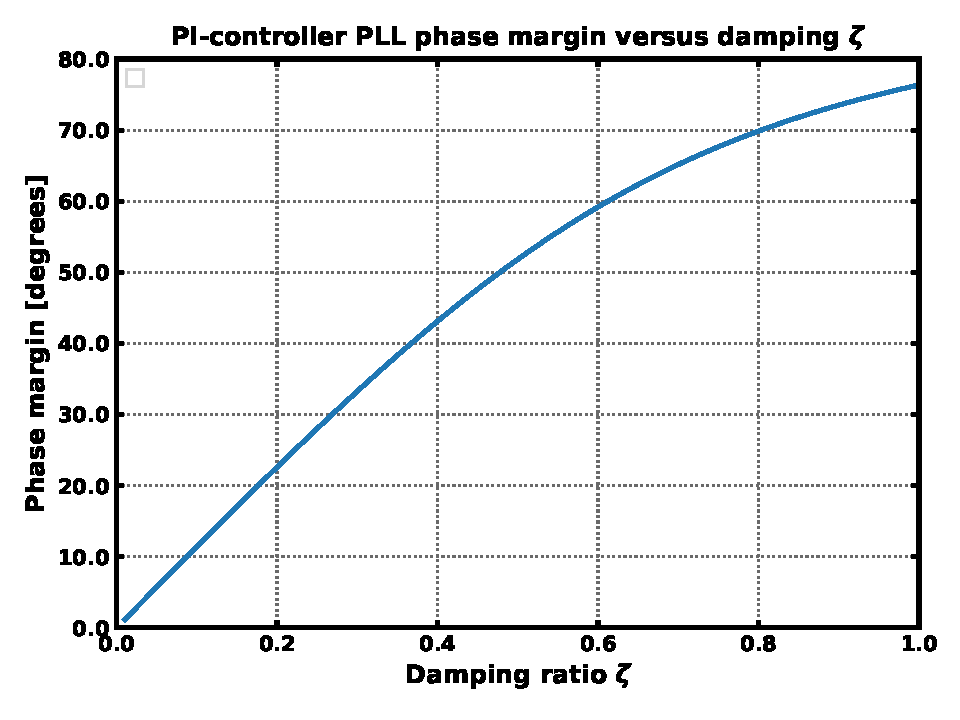
\includegraphics[width=0.5\textwidth, angle=0]{figs/damping_vs_pm.pdf}
				\caption{PI-controller PLL phase margin versus damping ratio.}
				\label{fig:phase_margin}
			\end{figure}

		\subsubsection{PI-controller peaking compensation}\label{comp_pi_pll_lf}
			 To compensate for closed loop peaking, the original PI-controller loop filter of equation \ref{eq:pi_pll_tf} can be modified with the addition of a single tunable pole at $\omega_p$. The closed loop response becomes third order, which complicates direct analysis and design of the loop filter, but can be handled utilizing the numerical optimization approach described in this work.
			 \hl{Not necessarily stable as closed loop configuration has 3 poles}
			\begin{equation} \label{eq:pi_compensated_tf}
				\textnormal{H}_{LF}(s) = \frac{K_i}{s}\frac{\left(\frac{s}{\omega_z} + 1\right)}{\left(\frac{s}{\omega_p} + 1\right)}
			\end{equation}

		\subsubsection{Alternative PID controller permutations} \label{other_pid}
			If individual terms within the PID-controller are dropped, different controller permutations (PD, ID, PI, P, I, D) can be achieved. As mentioned before, inclusion of an integral term is needed to ensure the desired zero steady state error for a PLL, and the derivative term must be removed to achieve low pass response in the PLL. This leaves integral term only controller as the remaining candidate for PID controller design. Thus, setting the $K_p$ and $K_d$ terms of equation \ref{eq:pid_pll_tf} to zero yields:
			\begin{equation}
				\frac{\Phi_{out}(s)}{\Phi_{ref}(s)} = \frac{2\pi K_{VCO}K_i}{s^2 + \frac{2\pi K_{VCO}}{\mathrm{N}}K_i}
			\end{equation}
			This closed loop transfer function results in a pair of poles at $\pm\sqrt{2\pi K_{VCO}K_i/\mathrm{N}}$. This is not stable, as it can only be manifested as (1) a pair of poles on the imaginary axis, which is an oscillator, or (2) a real pole in the right-half plane and a real pole in the left-half plane, the former of which is not causally stable. Thus a PI-controller is the only viable PID-controller permutation for use in a PLL loop filter. 


	\subsubsection{Discretized Loop Filter Prototype}\label{disc_lf_comp_pi}
		Using the continuous filter discretization approach described in section \ref{lf-discretization} on the loop filter of equation \ref{eq:pi_compensated_tf} results in equation \ref{eq:z_lf}.
		\begin{align}
			\textnormal{H}_{LF}(z) & = \left.\frac{K_i}{s}\frac{\left(\frac{s}{\omega_z} + 1\right)}{\left(\frac{s}{\omega_p} + 1\right)}\right\vert_{s=\frac{1}{\Delta T_s}(1-z^{-1})}
			&= k_i\Delta T_s\frac{\omega_p}{\omega_z}\frac{(1+\omega_z\Delta T_s)-z^{-1}}{(1+\omega_p\Delta T_s) - z^{-1}(2+\omega_p\Delta T_s) + z^{-2}}\label{eq:z_lf}
		\end{align}

		The transformation of \ref{eq:z_lf} into a digitally implementable design as a direct form 1 IIR filter shown in figure \ref{fig:filt_imple}. Its filter coefficients given by equations \ref{eq:a1}-\ref{eq:b1}.
		\begin{figure}[htb!]
			\center\fontfamily{\sfdefault}\selectfont
% XCircuit output "filter_arch_tex.tex" for LaTeX input from filter_arch_tex.ps
\def\putbox#1#2#3#4{\makebox[0.00000in][l]{\makebox[#1][l]{}\raisebox{\baselineskip}[0.00000in][0.00000in]{\raisebox{#2}[0.00000in][0.00000in]{\scalebox{#3}{#4}}}}}
\def\rightbox#1{\makebox[0.00000in][r]{#1}}
\def\centbox#1{\makebox[0.00000in]{#1}}
\def\topbox#1{\raisebox{-0.60\baselineskip}[0.00000in][0.00000in]{#1}}
\def\midbox#1{\raisebox{-0.20\baselineskip}[0.00000in][0.00000in]{#1}}
   \scalebox{1}{
   \normalsize
   \parbox{5.54167in}{
   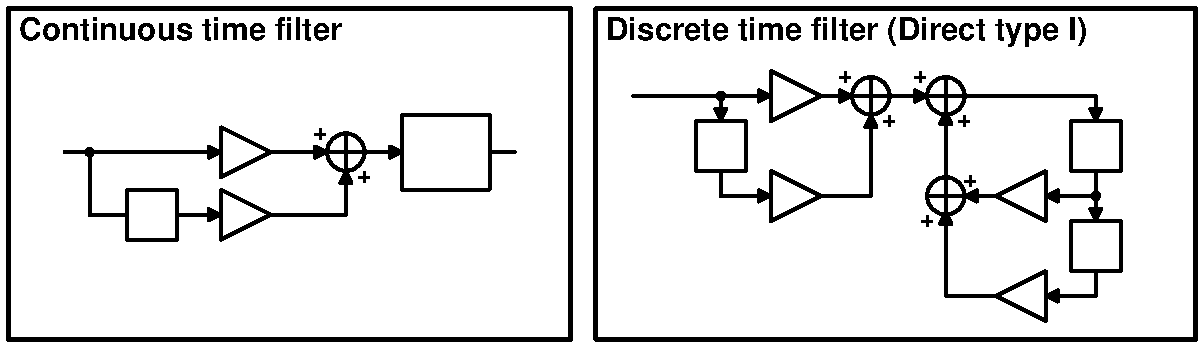
\includegraphics[scale=0.70000]{./figs/filter_arch_tex.pdf}\\
   % translate x=1728 y=944 scale 0.38
   \putbox{1.91800in}{0.90300in}{0.96}{$\frac{1}{\frac{s}{\omega_p} + 1}$}%
   \putbox{1.14800in}{1.01500in}{0.96}{$K_p$}%
   \putbox{1.14800in}{0.72800in}{0.96}{$K_i$}%
   \putbox{0.60900in}{0.58100in}{0.96}{$1/s$}%
   \putbox{0.25900in}{0.98700in}{0.96}{x[n]}%
   \putbox{2.35900in}{0.98700in}{0.96}{y[n]}%
   \putbox{2.92600in}{1.25300in}{0.96}{x[n]}%
   \putbox{5.17300in}{1.16200in}{0.96}{y[n]}%
   \putbox{3.26200in}{0.90300in}{0.96}{$z^{-1}$}%
   \putbox{3.73100in}{1.28100in}{0.96}{b$_0$}%
   \putbox{3.73100in}{0.81200in}{0.96}{b$_1$}%
   \putbox{5.01200in}{0.90300in}{0.96}{$z^{-1}$}%
   \putbox{5.01200in}{0.43400in}{0.96}{$z^{-1}$}%
   \putbox{4.60600in}{0.82600in}{0.96}{-a$_1$}%
   \putbox{4.59200in}{0.35700in}{0.96}{-a$_2$}%
   \putbox{5.17300in}{0.69300in}{0.96}{y[n-1]}%
   \putbox{5.15900in}{0.23100in}{0.96}{y[n-2]}%
   } % close 'parbox'
   } % close 'scalebox'
   \vspace{-\baselineskip} % this is not necessary, but looks better
\fontfamily{\rmdefault}\selectfont

			\caption{Implementation of filter.}
			\label{fig:filt_imple}
		\end{figure}
					% y[n] = x[n]\frac{K_i\omega_pT}{\omega_z}\frac{1+\omega_zT}{1+\omega_pT} - x[n-1]\frac{K_i\omega_pT}{\omega_z}\frac{1}{1+\omega_pT} + y[n-1]\frac{2+\omega_pT}{1+\omega_pT} - y[n-2]\frac{1}{1+\omega_pT}\\
					% = a_0x[n] + a_1x[n-1] - b_1y[n-1] - b_2x[n-2] 
		\begin{align}
			a_1 &= -\frac{2+\omega_p\Delta T_s}{1+\omega_p\Delta T_s}\label{eq:a1} 
			& a_2 &= \frac{1}{1+\omega_p\Delta T_s} \\
			b_0 &= \frac{K_i\omega_p\Delta T_s}{\omega_z}\frac{1+\omega_z\Delta T_s}{1+\omega_p\Delta T_s}
			& b_1 &= \frac{K_i\omega_p\Delta T_s}{\omega_z}\frac{1}{1+\omega_p\Delta T_s}\label{eq:b1}
		\end{align}

		%%%%

		\subsubsection{Prototype PLL response}\label{proto_pll_tfs}
		Based on the prototype loop filter developed, the PLL closed loop response is developed for usage in the loop optimizer discussed in this work. Applying the discrete-time PLL transfer function model developed in section \ref{discrete_pll_tf}, the PLL loop gain is in equation \ref{eq:z_loop_gain_pi_comp}, and the closed loop transfer function of the PLL is in \ref{eq:z_cl_tf_pi_comp_pll}.
		\begin{align}
			\mathrm{L}(z) &= \mathrm{H}_{TDC}(z)\mathrm{H}_{LF}(z)\mathrm{H}_{DCO}(z)\mathrm{H}_{DIV}(z) \\
			&= 2\pi K_{DCO}K_i\Delta T_s^2\frac{\mathrm{M}}{\mathrm{N}}\frac{\omega_p}{\omega_z}\frac{(1+\omega_z\Delta T_s)-z^{-1}}{(1+\omega_p\Delta T_s) - z^{-1}(3+2\omega_p\Delta T_s) + z^{-2}(3+\omega_p\Delta T_s) - z^{-3}}\label{eq:z_loop_gain_pi_comp}
		\end{align}
		The closed loop z-domain PLL phase transfer function is:
		\begin{align}\label{eq:z_cl_tf_pi_comp_pll}
			\mathrm{T}(z) = \frac{\Phi_{out}(z)}{\Phi_{ref}(z)} &= \frac{2\pi K_{DCO}K_i\Delta T_s^2\mathrm{M}\frac{\omega_p}{\omega_z}(1+\omega_z\Delta T_s)-z^{-1}}{\left(\parbox{4.2in}{$(1+\omega_p\Delta T_s + 2\pi K_{DCO}K_i\Delta T_s^2\frac{\mathrm{M}}{\mathrm{N}}\frac{\omega_p}{\omega_z}(1+\omega_z\Delta T_s))- z^{-1}(3+2\omega_p\Delta T_s+2\pi K_{DCO}K_i\Delta T_s^2\frac{\mathrm{M}}{\mathrm{N}}\frac{\omega_p}{\omega_z})+ z^{-2}(3+\omega_p\Delta T_s) - z^{-3}$}\right)}%\\
			%&= \mathrm{N}\frac{\mathrm{L}(z)}{1+\mathrm{L}(z)}\\
		\end{align}
		Applying z-to-s domain transformation, the continuous s-domain approximation of the loop gain is given in equation \ref{eq:s_loop_gain_pi_comp}, and the closed loop transfer function in equation \ref{eq:s_cl_tf_pi_comp_pll}.
		\begin{align}
			\mathrm{L}(s) = \mathrm{H}_{TDC}(s)\mathrm{H}_{LF}(s)\mathrm{H}_{DCO}(s)\mathrm{H}_{DIV}(s) = \frac{\mathrm{M}}{\mathrm{N}}\frac{K_{DCO}K_i}{s^2} \frac{\left(\frac{s}{\omega_z} + 1\right)}{\left(\frac{s}{\omega_p} + 1\right)}\label{eq:s_loop_gain_pi_comp}
		\end{align}
		\begin{align}\label{eq:s_cl_tf_pi_comp_pll}
			\mathrm{T}(s)=\frac{\Phi_{out}(s)}{\Phi_{ref}(s)} = \frac{\mathrm{M}K_{DCO}K_i\left(\frac{s}{\omega_z} + 1\right)}{s^3\frac{1}{\omega_z} + s^2 + \frac{\mathrm{M}}{\mathrm{N}}K_{DCO}K_i\left(\frac{s}{\omega_z} + 1\right)} = \mathrm{N}\frac{\mathrm{L}(s)}{1+\mathrm{L}(s)} 
		\end{align}



%%%%%%%%%%%%%%%%%%%%%%%%%%%%%%%%%%%%%%%%%%%%%%%%%%%%%%%%%%%%%%%%%%%%
\pagebreak
\section{Behavioral ADPLL simulation}
To fully capture the effects of a discrete time PLL with digital quantization effects, the implementation of a behavioral, discrete event PLL simulator is described in the following. The simulator utilizes behavioral models to describe the individual components which comprise the PLL. These components are (1) a clock reference, (2) a TDC, (3) a loop filter, (4) a DCO, and (5) a divider. These behavioral models fully encapsulate effects of time-quantization and digitization. The simulator operates by iterating in fixed time steps of $\Delta t$=1/\texttt{fs}, where each node in the PLL is updated based upon the previous node values in a manner that is defined by each PLL component behavioral model. Each behavioral model is represented programmatically utilizing classes. In simulation, each component instance is represented by a object instance of the respective model class, constructed with any initial parameters (such as division ratio) that describe the component.
\subsection{Simulation engine}
The simulator engine for this work follows the sequence illustrated in figure \ref{fig:simulator} for running a simulation. Given specifications for simulation conditions (listed in the figure), the simulator accordingly initializes model objects that constitute the PLL components in simulation space. Then the simulation is run by entering a simulation loop. 
\begin{figure}[htb!]
	\center\fontfamily{\sfdefault}\selectfont
% XCircuit output "simulator.tex" for LaTeX input from simulator.ps
\def\putbox#1#2#3#4{\makebox[0.00000in][l]{\makebox[#1][l]{}\raisebox{\baselineskip}[0.00000in][0.00000in]{\raisebox{#2}[0.00000in][0.00000in]{\scalebox{#3}{#4}}}}}
\def\rightbox#1{\makebox[0.00000in][r]{#1}}
\def\centbox#1{\makebox[0.00000in]{#1}}
\def\topbox#1{\raisebox{-0.60\baselineskip}[0.00000in][0.00000in]{#1}}
\def\midbox#1{\raisebox{-0.20\baselineskip}[0.00000in][0.00000in]{#1}}
   \scalebox{1}{
   \normalsize
   \parbox{6.30936in}{
   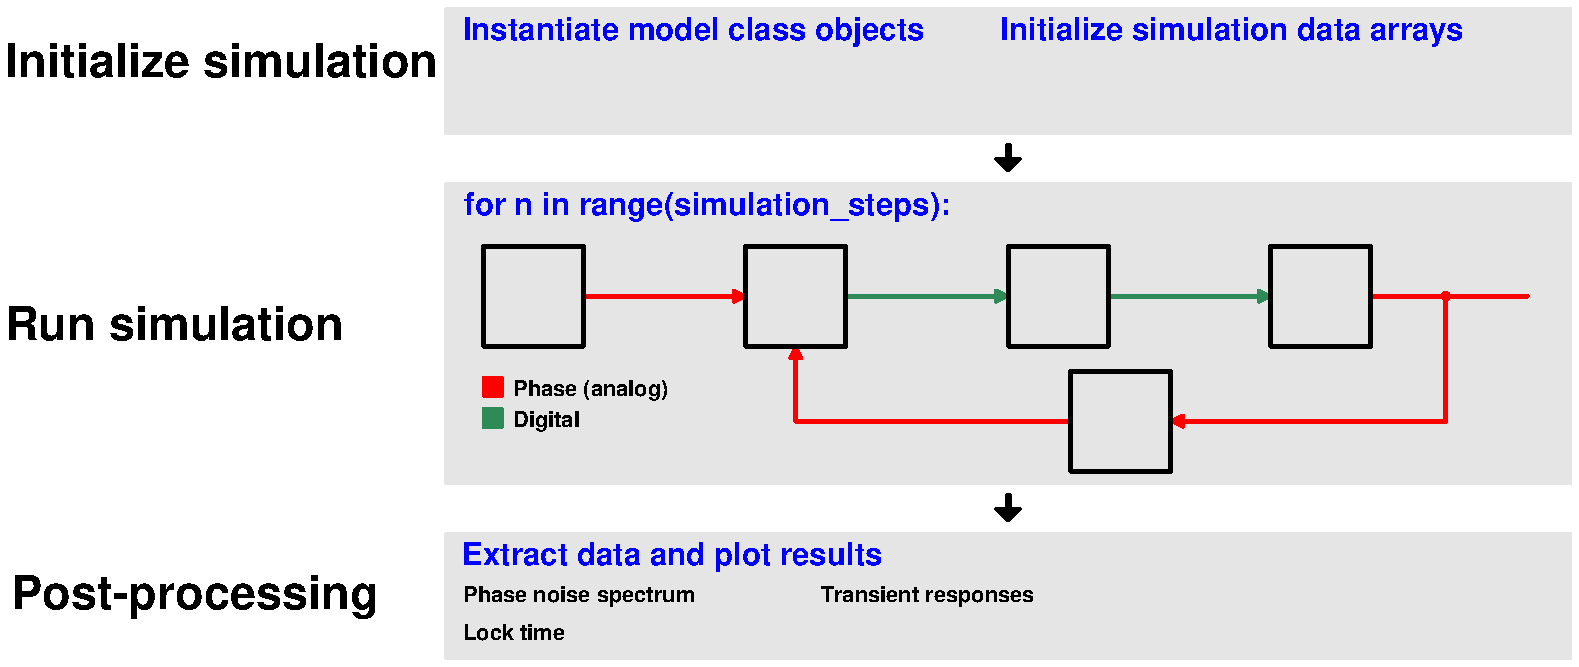
\includegraphics[scale=0.60000]{./figs/simulator.pdf}\\
   % translate x=1040 y=384 scale 0.38
   \putbox{3.08400in}{1.45800in}{0.84}{\texttt{tdc}}%
   \putbox{4.38600in}{0.96000in}{0.84}{\texttt{div}}%
   \putbox{4.17000in}{1.45800in}{0.84}{\texttt{lf}}%
   \putbox{5.18400in}{1.45800in}{0.84}{\texttt{dco}}%
   \putbox{2.03400in}{1.45800in}{0.84}{\texttt{clk}}%
   \putbox{3.48600in}{1.03200in}{0.84}{\texttt{div\_sig[n]}}%
   \putbox{2.38200in}{1.56000in}{0.84}{\texttt{clk\_sig[n]}}%
   \putbox{3.43200in}{1.54800in}{0.84}{\texttt{tdc\_sig[n]}}%
   \putbox{4.48200in}{1.54800in}{0.84}{\texttt{lf\_sig[n]}}%
   \putbox{5.53200in}{1.54800in}{0.84}{\texttt{dco\_sig[n]}}%
   \putbox{4.00800in}{2.35800in}{0.84}{\texttt{clk\_sig[n]}}%
   \putbox{4.00800in}{2.20800in}{0.84}{\texttt{tdc\_sig[n]}}%
   \putbox{4.71000in}{2.35800in}{0.84}{\texttt{lf\_sig[n]}}%
   \putbox{4.71000in}{2.20800in}{0.84}{\texttt{dco\_sig[n]}}%
   \putbox{5.38200in}{2.35800in}{0.84}{\texttt{div\_sig[n]}}%
   \putbox{1.86000in}{2.35800in}{0.84}{\texttt{clk}}%
   \putbox{1.86000in}{2.20800in}{0.84}{\texttt{tdc}}%
   \putbox{2.40600in}{2.35800in}{0.84}{\texttt{lf}}%
   \putbox{2.40600in}{2.20800in}{0.84}{\texttt{dco}}%
   \putbox{2.95800in}{2.35800in}{0.84}{\texttt{div}}%
   \putbox{1.88400in}{0.83400in}{0.84}{t$_{sim}$ = \texttt{n}$\Delta$t}%
   \putbox{2.73600in}{3.09600in}{0.72}{\texttt{fref}}%
   \putbox{2.55600in}{2.99400in}{0.72}{\texttt{div\_n}}%
   \putbox{2.49600in}{2.89800in}{0.72}{\texttt{tdc\_steps}}%
   \putbox{3.60600in}{3.09600in}{0.72}{\texttt{kdco}}%
   \putbox{4.20600in}{2.99400in}{0.72}{\texttt{dco\_f0}}%
   \putbox{4.20600in}{2.89800in}{0.72}{\texttt{dco\_pn}}%
   \putbox{5.64600in}{3.09600in}{0.72}{\texttt{init\_f\_error}}%
   \putbox{5.18400in}{2.99400in}{0.72}{\texttt{lf\_params}}%
   \putbox{5.44800in}{2.89800in}{0.72}{\texttt{sim\_steps}}%
   } % close 'parbox'
   } % close 'scalebox'
   \vspace{-\baselineskip} % this is not necessary, but looks better
\fontfamily{\rmdefault}\selectfont

	\caption{Simulation process.}
	\label{fig:simulator}
\end{figure}
\FloatBarrier
The discrete event simulator loop is given in the following pseudocode of listing \ref{sim_code}, with component model objects \{\texttt{clk, tdc, lf, dco, div}\}, and simulation data arrays \{\texttt{clk\_sig, tdc\_sig, lf\_sig, dco\_sig, div\_sig}\}. The simulation operates with a fixed, discrete time step. Each model object is updated at each simulation step (loop iteration) utilizing the class method \texttt{update}, passing any relevant simulation data as arguments to the method. The output state of each component is saved into the respective array instance for each simulation step. 

\begin{lstlisting}[language={Python}, caption={PLL simulation loop Python pseudocode}, label={sim_code}]
for n in range(simulation_steps):
    clk_sig[n] = clk.update()
    tdc_sig[n] = tdc.update(clk_sig[n-1], div_sig[n-1]))
    lf_sig[n]  = lf.update(tdc_sig[n-1], clk_sig[n-1]) #loop filter
    osc_sig[n] = dco.update(lf_sig[n-1])
    div_sig[n] = div.update(osc_sig[n-1], div_n)
    \end{lstlisting}
After the simulation loop reaches completion, the results stored in the simulation data arrays can be post-processed to extract phase noise data, transient behavior and lock time. The following sections will discuss in more detail the implemented behavioral model classes and post-processing.

\subsection{Clock behavioral model}
An ideal behavioral clock model is utilized, given in the pseudocode of listing \ref{clk_code}. The model is instantiated with the clock frequency \texttt{f} and the simulator time step \texttt{dt}. The model incrementing its phase every simulation step by a fixed amount $\Delta \Phi$ = $2\pi$\texttt{f}$\cdot$\texttt{dt}, as in \ref{eq:clk_behavioral_model}. The model outputs an analog phase signal.
\begin{equation}\label{eq:clk_behavioral_model}
	\Phi_{clk}[n] = \Phi_{clk}[n-1] + 2\pi\mathtt{f}\cdot\mathtt{dt}
\end{equation}

\begin{lstlisting}[language={Python}, caption={Ideal clock behavioral model Python pseudocode.}, label={clk_code}]
class Clock:
	def __init__(self, f, dt):
		self.f = f 			# clock frequency
		self.dt = dt 		# simulation time step
		self.phase = 0.0	# clock phase state variable

	def update(self):
		self.phase += 2*pi*self.f*self.dt 	# increment phase
		return self.phase
    \end{lstlisting}

\subsection{TDC behavioral model}
The TDC behavioral model takes two analog inputs \texttt{x} and \texttt{y} that are in units of phase, and outputs a digital word that quantifies the phase separation of the signals. The model is instantiated with a resolution parameter \texttt{tdc\_steps}, which defines the number of phase steps per cycle of the reference input \texttt{x} the TDC can resolve. The method \texttt{round} quantizes an floating point argument to the nearest integer.
\begin{equation}
	\text{out}[n] = \left\lfloor0.5 + \mathtt{tdc\_steps}\frac{\mathtt{x}[n]-\mathtt{y}[n]}{2\pi} \right\rfloor
\end{equation}

\begin{lstlisting}[language={Python}, caption={TDC behavioral model Python pseudocode.}, label={tdc_code}]
class TDC:
	def __init__(self, tdc_steps):
		self.tdc_steps = tdc_steps

	def update(x, y):
		ph_error = wrap(x-y) 	# wraps phase to be within [0, 2*pi]
		return round(self.tdc_steps*(ph_error/(2*pi)))
\end{lstlisting}
\subsection{Loop filter behavioral model}
The loop filter model implements a discrete-time filter via difference equation that operates on input \texttt{x}. The equivalent of one pole and two zeros are modelled, described using the filter coefficients $\{a_1, a_2; b_0, b_1\}$:
\begin{equation}
\text{H}_{LF}(z) = \frac{b_0 + b_1z^{-1}}{a_0 + a_1z^{-1} + a_2z^{-2}}
\end{equation}
\begin{equation}
\text{y}[n] = -a_1 \text{y}[n-1]-a_2 \text{y}[n-2] + b_0\text{x}[n] + b_1\text{x}[n-1]
\end{equation}
Pseudocode for implementation of the model class is as follows. Data is to be represented with fixed point format, with number of fractional bits \texttt{frac\_bits} and number of integer bits \texttt{int\_bits}. The method \texttt{fixed\_point} rounds floating point values to be equivalent to the nearest representation in the desired fixed point format. The filter coefficients are assumed to be pre-converted to the desired fixed-point equivalent values, and input \texttt{x} is assumed to be integer-valued.
\begin{lstlisting}[language={Python}, caption={Loop filter behavioral model Python pseudocode.}, label={lf_code}]
class LoopFilter:
	def __init__(self, a1, a2, b0, b1, int_bits, frac_bits):
		self.a1 = a1;	self.a2 = a2
		self.b0 = b0;	self.b1 = b1
		self.xprev1 = 0;	
		self.yprev1 = 0; self.yprev2 = 0
		self.int_bits=int_bits;	self.frac_bits=frac_bits

	def update(x):
		ynew = -self.a1*self.yprev1 - self.a2*self.yprev2 \\
			   + self.b0*x + self.b1*self.xprev1	# difference equation
		self.yprev2 = self.yprev1	
		self.yprev1 = fixed_point(ynew, self.int_bits, self.frac_bits)
		self.xprev1 = x
		return round(self.yprev1)	# convert to integer
\end{lstlisting}

\subsection{DCO behavioral model}
The DCO is modeled similar to the clock model, with the inclusion of a digital input \texttt{otw} for tuning the frequency. Nominal oscillator frequency is given by \texttt{f0}, and the DCO gain in Hz/LSB of \texttt{otw} is \texttt{kdco}. Additionally, modeling of the $\propto f^-2$ oscillator phase noise component, which is equivalent to random phase walk \cite{vannicola_varshney_1983}, is included utilizing additive random phase walk. Random walk is implemented by stochastically either adding or subtracting a fixed magnitude random walk phase increment $\texttt{krw}$ to the oscillator phase every simulation step. The sign of \texttt{krw} is randomly chosen with equal probability for positive and negative (sampling a bi-delta distribution), implemented with the method \texttt{choice}.
\begin{equation}\label{eq:dco_behavioral_model}
	\Phi_{osc}[n] = \Phi_{osc}[n-1] + 2\pi(\mathtt{f0}+\mathtt{otw}\cdot\mathtt{kdco})\cdot\mathtt{dt} \pm \mathtt{krw}
\end{equation}
\begin{lstlisting}[language={Python}, caption={DCO behavioral model Python pseudocode.}, label={dco_code}]
class DCO:
	def __init__(self, f0, kdco, krw, dt):
		self.f0 = f0		# nominal frequency
		self.kdco = kdco 	# DCO gain
		self.krw			# random phase walk gain
		self.dt 			# simulation time step size
		self.phase = 0		# phase state variable

	def update(otw):
		self.phase += 2*pi*(self.f0 + otw*self.kdco)*self.dt + krw*choice([-1,1])
		return self.phase
   \end{lstlisting}

Selection of the parameter \texttt{krw} to achieve a target phase noise level $\mathcal{L}(\Delta f)$ at offset $\Delta f$ from the carrier is as follows.
	\begin{figure}[htb!]
	    \centering
	    \begin{subfigure}{0.45\textwidth}
	        \centering
			\fontfamily{\sfdefault}\selectfont
% XCircuit output "rw_pn.tex" for LaTeX input from rw_pn.ps
\def\putbox#1#2#3#4{\makebox[0.00000in][l]{\makebox[#1][l]{}\raisebox{\baselineskip}[0.00000in][0.00000in]{\raisebox{#2}[0.00000in][0.00000in]{\scalebox{#3}{#4}}}}}
\def\rightbox#1{\makebox[0.00000in][r]{#1}}
\def\centbox#1{\makebox[0.00000in]{#1}}
\def\topbox#1{\raisebox{-0.60\baselineskip}[0.00000in][0.00000in]{#1}}
\def\midbox#1{\raisebox{-0.20\baselineskip}[0.00000in][0.00000in]{#1}}
   \scalebox{1}{
   \normalsize
   \parbox{2.66666in}{
   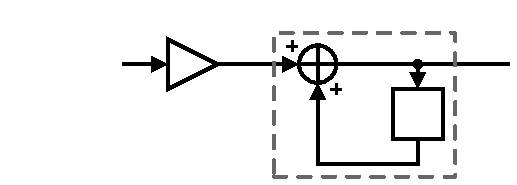
\includegraphics[scale=0.80000]{./figs/rw_pn.pdf}\\
   % translate x=924 y=776 scale 0.38
   \putbox{0.51200in}{0.71200in}{0.96}{w[n]}%
   \putbox{2.49600in}{0.72800in}{0.96}{y[n]}%
   \putbox{0.96000in}{0.79200in}{0.96}{\texttt{krw}}%
   \putbox{2.11200in}{0.32800in}{0.96}{$z^{-1}$}%
   \putbox{0.04800in}{0.51200in}{0.72}{...,+1,-1,-1,+1,...}%
   \putbox{1.83200in}{0.86400in}{0.96}{Integrator}%
   \putbox{1.19200in}{0.71200in}{0.96}{x[n]}%
   } % close 'parbox'
   } % close 'scalebox'
   \vspace{-\baselineskip} % this is not necessary, but looks better
\fontfamily{\rmdefault}\selectfont

			\caption{ }
			\label{fig:rw_pn}
	    \end{subfigure}
	    \begin{subfigure}{0.5\textwidth}
	        \centering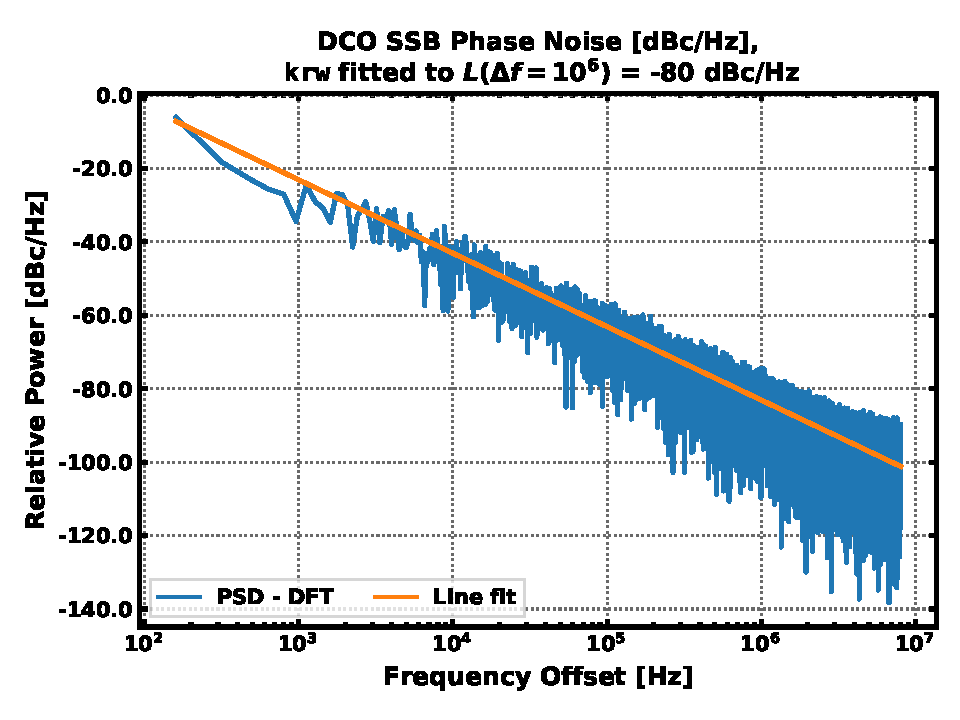
\includegraphics[width=1.0\textwidth, angle=0]{figs/dco_rw_pn.pdf}
			\caption{ }
			\label{fig:dco_rw_pn_sim}
	    \end{subfigure}%
	    \label{fig:dco_rw_model}
	    \caption{\textbf{(a)} Discrete model for oscillator random walk, \textbf{(b)} Simulated phase noise of behavioral model.}
	\end{figure}
	\FloatBarrier
The random walk process described in the behavioral model is represented in figure \ref{fig:rw_pn}, where a random white-spectrum input sequence $w$[n] taking on values $\pm$ 1 with equal probability are multiplied by gain \texttt{krw}, yielding signal $x$[n] that is passed a discrete integrator. The output $y$[n] is then the phase noise signal that is summed with the oscillator phase trajectory. If the simulation is limited to \texttt{sim\_steps} samples, application of Parseval's theorem for the discrete Fourier transform (DFT) of x[n] in \ref{eq:parsevals} results in the estimate of the energy spectrum x[n] \ref{eq:white_noise_pow}, having a constant value $\sigma_x^2$ .
\begin{equation}\label{eq:parsevals}
\sum _{n=0}^{\mathtt{sim\_steps}-1}|\texttt{krw}\cdot w[n]|^{2}=\frac{1}{\mathtt{sim\_steps}}\sum _{k=0}^{\mathtt{sim\_steps}-1}| X[k]|^{2}
\end{equation}
\begin{equation}\label{eq:white_noise_pow}
\sigma_x^2 = |X[k]|^{2} =\mathtt{sim\_steps}\cdot\texttt{krw}^2
\end{equation}

Computation of the spectrum of the output $y[n]$ of figure \ref{fig:rw_pn} can be computed as follows, recalling that $x[n]$ is white with power $\sigma_x^2$, and approximating $z = 1-s\mathtt{dt}$ is in \ref{eq:rw_model_pn_spectrum}. Normalizing $Y(f)$ by the number of samples \texttt{sim\_steps} to compute spectral density is performed in \ref{eq:rw_model_pn_spectrum_normed}.
\begin{equation}\label{eq:rw_model_pn_spectrum}
|Y(f)|^{2} = \left.|X(z)|^{2}\frac{1}{|1-z^{-1}|^2}\right|_{z^{-1}=(1-j2\pi f\mathtt{dt})} = \frac{\sigma_x^2}{|j2\pi f\mathtt{dt}|^2} = \frac{\mathtt{sim\_steps}\cdot\texttt{krw}^2}{(2\pi f\mathtt{dt})^2}
\end{equation}
\begin{equation}\label{eq:rw_model_pn_spectrum_normed}
|\hat Y(f)|^{2} = \frac{\texttt{krw}^2}{\mathtt{sim\_steps}\cdot(2\pi f\mathtt{dt})^2}
\end{equation}
Given the target phase noise level $\mathcal{L}(\Delta f)$ at offset $\Delta f$, we set $f=\Delta f$ and $|\hat Y(\Delta f)|^{2}$=$\mathcal{L}(\Delta f)$, a reorganization of \ref{eq:rw_model_pn_spectrum_normed} results in the final expression for \texttt{krw}, equation \ref{eq:krw}. Figure \ref{fig:dco_rw_pn_sim} demonstrates simulated a test of this behavioral model, for \texttt{krw} fitted to $\mathcal{L}(\Delta f=10^6)$ = -80 dBc/Hz.
\begin{equation}\label{eq:krw}
\texttt{krw} = 2\pi \Delta f\cdot\mathtt{dt}\sqrt{\mathcal{L}(\Delta f)\cdot\mathtt{sim\_steps}}
\end{equation}



\subsection{Divider behavioral model}
The divider model is defined with the divider modulus \texttt{div\_n} and only performs a simple division of input phase. 
\begin{lstlisting}[language={Python}, caption={Divider behavioral model Python pseudocode.}, label={div_code}]
class Divider:
	def update(x, div_n):
		return x/div_n
\end{lstlisting}

\subsection{Post processing: lock time detection}
Lock time detection of the PLL start-up transient can be determined from the simulation data conditioned on a tolerance band for acceptable frequency error \texttt{lock\_f\_tol} is provided to the simulator by the user. Since the desired frequency of the PLL \texttt{fosc = div\_n*fref}, nominal oscillator frequency \texttt{dco\_f0} and simulation conditions of the PLL are known by the simulator, the ideal value of the loop filter at lock, \texttt{lf\_lock\_ideal} can be computed directly. Given the DCO gain value in the simulation \texttt{kdco}, the value of \texttt{lf\_lock\_ideal = round((fosc - dco\_f0)/kdco)}. Lock is then detected at the first simulation step for which the current and all later time steps meet the following criteria for the loop filter signal \texttt{lf\_sig} (i.e. frequency of oscillator is within the frequency tolerance band):
\begin{equation}
\text{\texttt{abs(lf\_sig[n] - lf\_lock\_ideal)*kdco < lock\_f\_tol}}
\end{equation}
This measurement is predicated on the simulation being fully complete at the time of measurement. Lock time is computed by multiplying the simulation index of lock with the simulation time step, 1/\texttt{fs}. Figure \ref{fig:loop_filter_trans} demonstrates the lock detection technique.

\begin{figure}[htb!]
	\center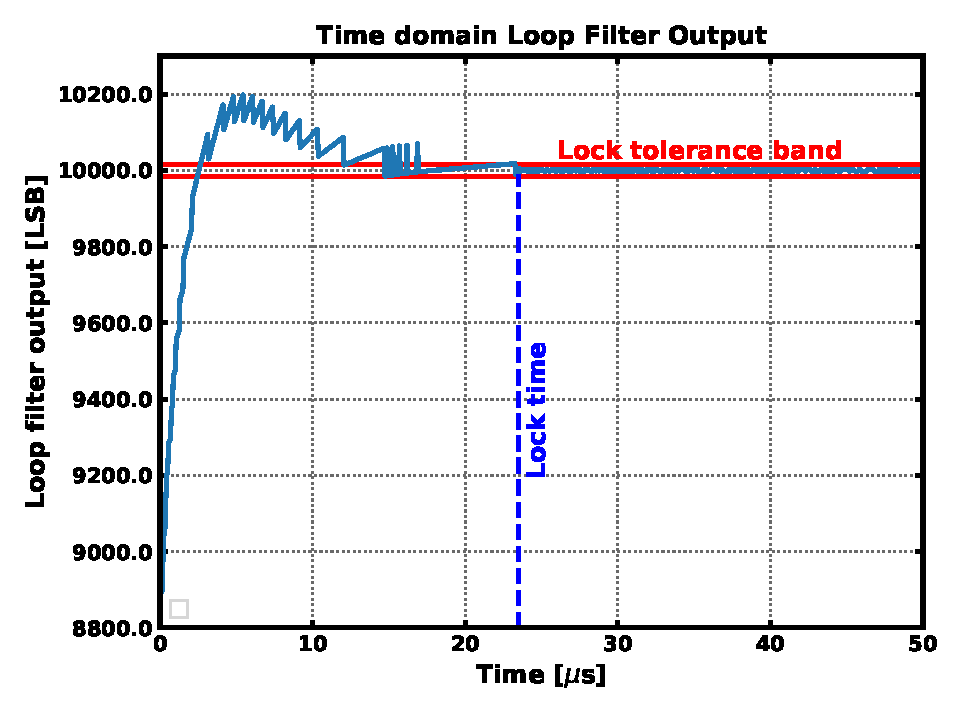
\includegraphics[width=0.5\textwidth, angle=0]{figs/loop_filter_trans.pdf}
	\caption{Detection of lock time from simulated PLL transient at loop filter.}
	\label{fig:loop_filter_trans}
\end{figure}
\FloatBarrier

\subsection{Post processing: phase noise power spectrum estimate}
The simulation data can be used to make an estimate of the phase noise power spectrum $\mathcal{L}(\Delta f)$ of the PLL (normalized to the carrier power). First, the phase error signal of the simulated PLL must be computed, \texttt{phase\_error = div\_n*clk\_sig - osc\_sig}. The phase error signal includes the phase noise signal in addition to any transient phase error components of the PLL. If the simulated PLL is in lock, the phase error can be is dominated by phase noise components, as the transient components become negligible. If \texttt{phase\_error} is reduced to the simulation signal span after the detection of lock, with a span in samples of \texttt{n\_steps}, the power spectral density of the phase noise normalized to the carrier tone, utilizing the fast Fourier transform (FFT) is in \ref{eq:psd_estimate}. This definition is based on the FFT implementation available in \texttt{numpy.fft} \cite{numpy.fft}.
\begin{equation}\label{eq:psd_estimate}
	\text{\texttt{psd}} = \left|\frac{1}{\text{\texttt{n\_steps}}}\cdot\mathcal{FFT}\{\text{\texttt{div\_n*clk\_sig - osc\_sig}}\}\right|^2
\end{equation}
Provided the simulation sampling rate \texttt{fs}, the indices [0, \texttt{n\_steps}/2-1] of the FFT and consequently \texttt{psd} correspond to frequencies [0, \texttt{fbin}$\cdot$(\texttt{n\_steps}/2-1)], where \texttt{fbin} = \texttt{fs}/\texttt{n\_steps}. Slicing the power spectrum data \texttt{psd} with indices [1, \texttt{fbin}$\cdot$(\texttt{n\_steps}/2-1)] will yield the single side band spectrum of the oscillator, with the corresponding offset frequency of each index \texttt{k} being $\Delta f\cdot \mathtt{k}\cdot\mathtt{fbin}$. Thus:
\begin{equation}
	\mathcal{L}(\Delta f) = \text{\texttt{psd[round(}}\Delta f\text{\texttt{/fbin)]}}
\end{equation}

Computation of power spectrum based on the DFT has high variance about the true spectrum, thus an additional approach utilized here is parametric spectral estimation with autoregressive (AR) model \cite{proakis_1993_psd}, which allows for lower variance of the estimate. An AR(p) model is simply a transfer function with p poles, which can be minimum mean square error (MMSE) optimized to fit the spectrum of a signal. The MMSE optimization for an AR model can be performed using linear algebra with the Yule-Walker equations, which is based on the autocorrelation sequence of the signal to be fitted (see appendix \ref{yule_walker_ar_psd}). This approach is utilized in this work. Figure \ref{fig:psd_est} shows example power spectrum estimates utilizing the two implemented methods on a test data set.

	\begin{figure}[htb!]
		\center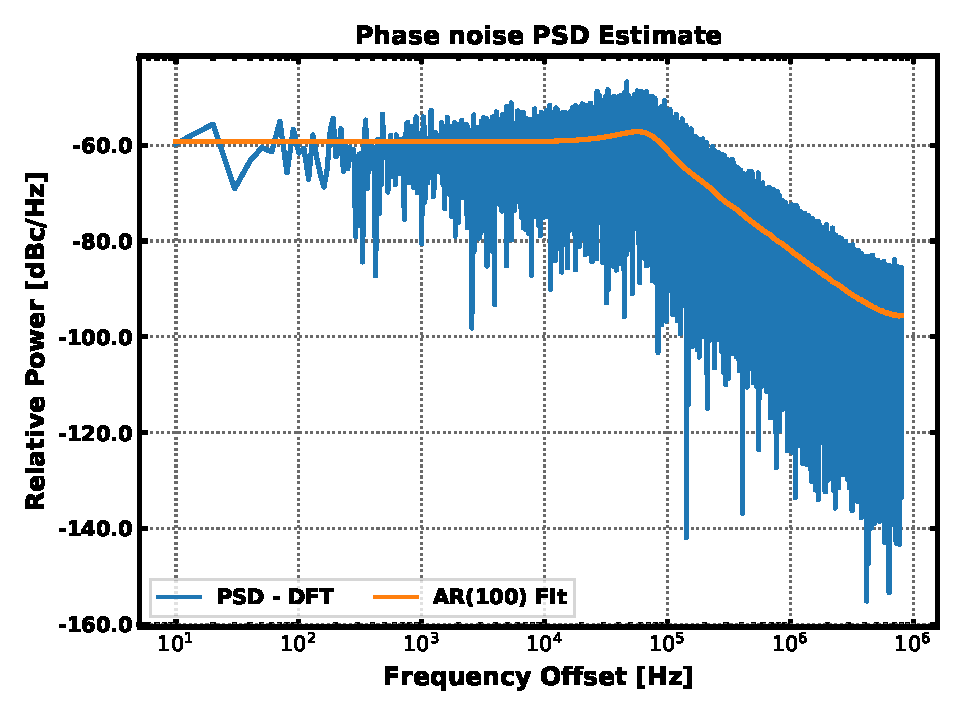
\includegraphics[width=0.5\textwidth, angle=0]{figs/psd_estimate.pdf}
		\caption{Power spectrum estimates example.}
		\label{fig:psd_est}
	\end{figure}
	\FloatBarrier

\subsection{Monte-Carlo sampling}
The simulation code implemented uses a Python dictionary containing the simulation parameters and the corresponding parameters for which the simulation engine should simulate the PLL for. This format makes the introduction of Monte-Carlo sampling into the simulator straightforward. This can be implementing utilizing a dictionary with the nominal simulation configuration, and then a second dictionary to define the parameters to be varied along with the corresponding parameter variance. Given a sample size of N for the Monte-Carlo simulation, a loop is implemented which creates a new simulation configuration dictionary each loop iteration with stochastically sampled values from a normal distribution based on the provided nominal configuration and variance dictionaries. That unique configuration dictionary instance is used to spawn a PLL simulation, and is stored. After N iterations, N sets of data are created with varied parameters.



%%%%%%%%%%%%%%%%%%%%%%%%%%%%%%%%%%%%%%%%%%%%%
\pagebreak
\section{Loop filter optimization}\label{methods_lf_opt}
The loop filter optimization engine implemented  minimizes total phase noise power of a PLL subject to a maximal lock time constraint. The optimizer uses a fixed prototype design for the loop filter in the form of equation \ref{eq:loop_filter_def} arrived at in section \ref{comp_pi_pll_lf} with parameters $\{K_i$, $\omega_p$, $\omega_z\}$. Based on section \ref{proto_pll_tfs}, the PLL developed in this work will have open loop and normalized and continuous closed loop transfer functions $\mathrm{L}(s)$ and $\mathrm{\hat{T}}(s)$ in \ref{eq:pll_tf_def}. The parameter $K$ is equivalent to $\frac{\mathrm{M}}{\mathrm{N}}K_{DCO}K_i$, where M is the TDC resolution in steps, N is the divider ratio, $K_{DCO}$ is the DCO gain in Hz/LSD and $K_i$ is the loop filter integral term gain. 

	\begin{equation}\label{eq:loop_filter_def}
	\mathrm{H}_{LF}(s) = \frac{K_i}{s}\frac{(\frac{s}{\omega_z}+1)}{(\frac{s}{\omega_p}+1)}
	\end{equation}
	\begin{align}\label{eq:pll_tf_def}
	\mathrm{L}(s) = \frac{K}{s^2}\frac{(\frac{s}{\omega_z}+1)}{(\frac{s}{\omega_p}+1)},
	&&K=\frac{\mathrm{M}}{\mathrm{N}}K_{DCO}K_i,
	&&\mathrm{\hat{T}}(s) = \frac{\mathrm{L}(s)}{1+\mathrm{L}(s)}
	\end{align}

The filter optimization and design sequence is detailed below. The following sections cover this in more detail. 

\begin{enumerate}[itemsep=0pt,label=\protect\mycirc{\arabic*}]
	\setlength\itemsep{-0.8em}
	\item Optimize parameters $\{K, \omega_p, \omega_z\}$ of $\mathrm{\hat{T}}(s)$ for minimize total PLL phase noise power, using the phase noise model developed in section \ref{final_pn_model} parameterized by the transfer function $\mathrm{\hat{T}}(s)$ and PLL parameters $\{\mathrm{M},\mathrm{N},K_{DCO},S_{0\Phi n_{DCO}}\}$.
	\item Translate optimal parameters $\{K, \omega_p, \omega_z\}$ to prototype loop filter parameters $\{K_i, \omega_p, \omega_z\}$, perform continuous to discrete time filter conversion.
	\item Optimize fixed point resolution of digital loop filter implementation for finite word effects.
\end{enumerate}

% \begin{figure}[htb!]
% 	\center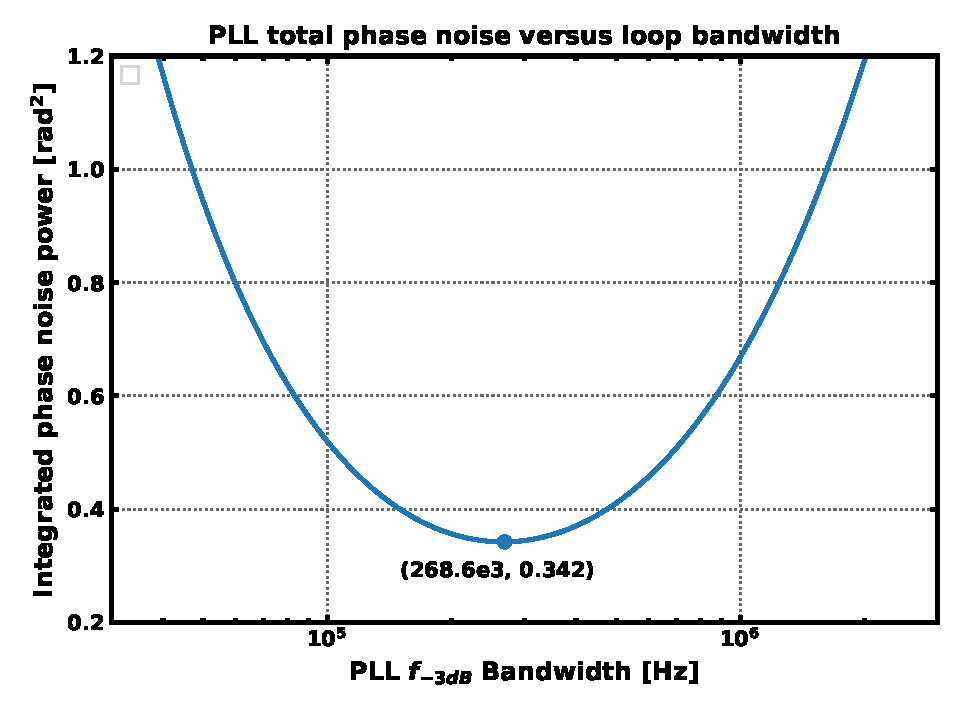
\includegraphics[width=0.5\textwidth, angle=0]{figs/bandwidth_vs_pn.pdf}
% 	\caption{Bandwidth versus total integrated phase noise of PLL.}
% 	\label{fig:bw_vs_pn}
% \end{figure}
% \FloatBarrier
\subsection{Optimization rationale}
The ADPLL transfer function in use (equation \ref{eq:pll_tf_def}), coupled with the phase noise theory of section \ref{final_pn_model} results in an output PLL phase noise spectrum with component-wise breakdown of figure \ref{fig:ex_pll_pn_comps}. The showing figure uses an arbitrary selection of PLL and phase noise parameters, however, varying the model parameters will shift the individual components up and in power and frequency. It is important to note in the presented PLL design, TDC, divider and loop filter phase noise components are manifested with a low pass response, and the DCO noise with a band pass response. Also note the overall PLL response is low pass, owing to the low pass nature of the loop filter. Figure \ref{fig:bw_pn_tradeoff} shows the result of integrating the phase noise spectrum to yield total PLL phase noise power for the system modeled in figure \ref{fig:ex_pll_pn_comps}. The parameters of the PLL were varied to change the half-power bandwidth of the closed loop response, resulting in a plot of total phase noise power versus PLL loop bandwidth. Here it is seen that there is an \textit{optimal} selection of bandwidth that minimizes phase noise power; and that loss function for this optimization, i.e. the total phase noise power, is convex, and thus is easily optimizable. 
	\begin{figure}[htb!]
	    \centering
	    \begin{subfigure}{0.5\textwidth}
	        \centering
	        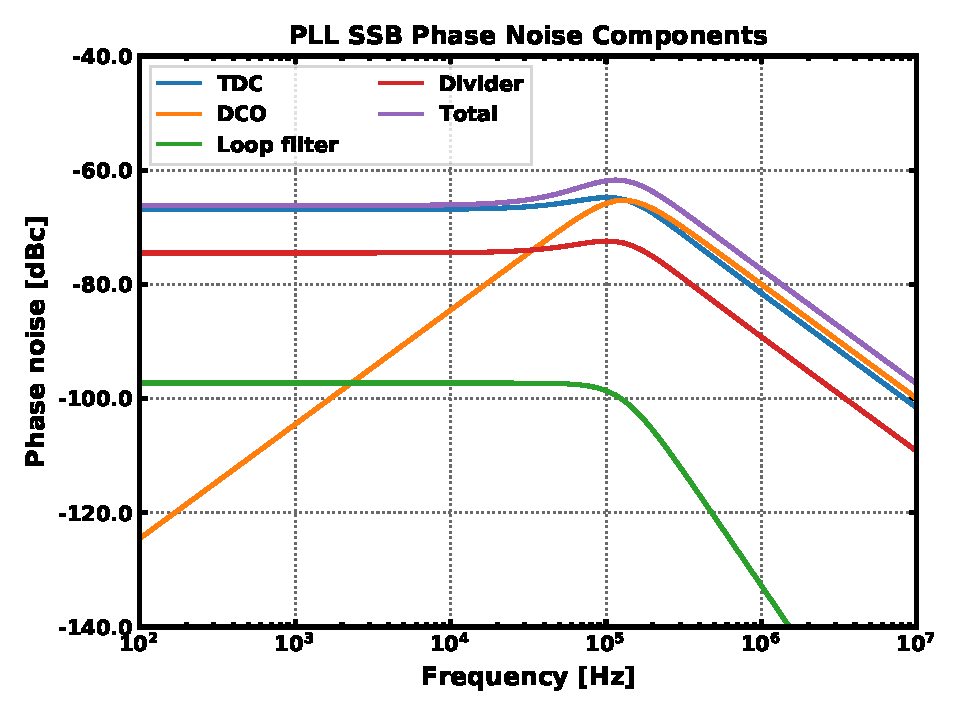
\includegraphics[width=1\textwidth, angle=0]{figs/pn_comps.pdf}
	        \caption{ }
	        \label{fig:ex_pll_pn_comps}
	    \end{subfigure}%
	    \begin{subfigure}{0.5\textwidth}
	        \centering
	        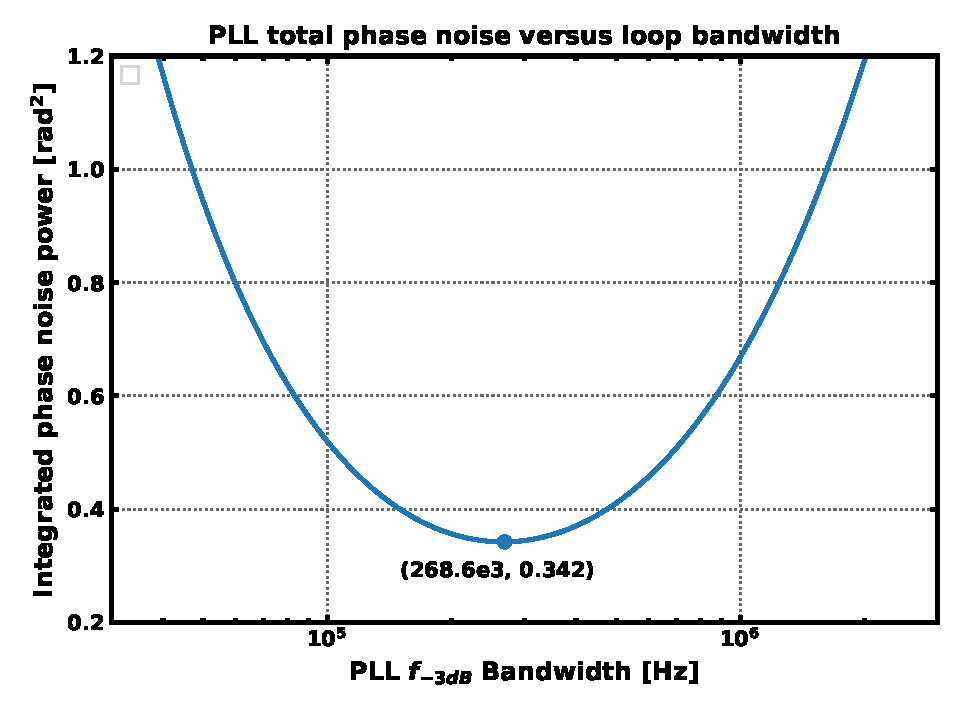
\includegraphics[width=1\textwidth, angle=0]{figs/bandwidth_vs_pn.pdf}
	        \caption{ }
	        \label{fig:bw_pn_tradeoff}
	    \end{subfigure}
	    % \caption{Approximate model for ring oscillator inverter delay cell.}
	    \label{fig:pll_pn_examples}
	    \caption{\textbf{(a)} Example PLL phase noise from models in this work, \textbf{(b)} integrated phase noise power versus bandwidth for the same PLL.}
	\end{figure}

The take-away here is the PLL will have an optimal set of parameters which will minimize the overall PLL phase noise. There is then a question of criteria for optimization. In the optimizer introduced here, the TDC and DCO phase noise are assumed to be the principal phase noise components, and are used as the sole criteria for establishing phase noise optimality. This assumption follows that the loop filter and divider implementations can be tuned easily to have less phase noise than DCO and TDC. This will be discussed in more detail later. If the TDC and DCO parameters are kept fixed, but the loop filter is varied resulting in a change of PLL bandwidth, figure \ref{fig:bw_vs_pn2} illustrates the corresponding changes in the DCO and TDC phase noise components. At low bandwidths, DCO noise because dominant, and at high bandwidths the TDC noise is dominant. In both cases, the total integrated phase noise is high (sub-optimal) due to excessive contributions from either component. Optimal bandwidth occurs when the contributions from both sources are approximately equal. It is possible that the optimal bandwidth for phase noise does not result in the desired transient lock time for the PLL, thus the final criteria for optimality is defined as \textit{the filter configuration that minimizes integrated TDC and DCO phase noise subject to a constraint for maximum lock time.}

\begin{figure}[htb!]
	\center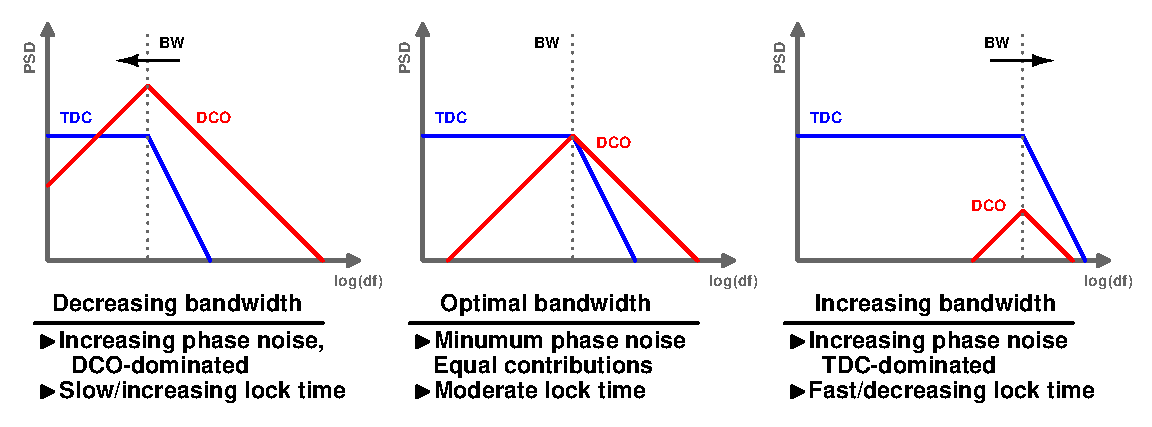
\includegraphics[width=1\textwidth, angle=0]{figs/loop_bandwidth}
	\caption{Bandwidth versus total integrated phase noise of PLL.}
	\label{fig:bw_vs_pn2}
\end{figure}


\subsection{Loop filter optimization algorithm}
Based on the developed criteria for PLL optimality, the following algorithm is defined to establish the optimal parameters $\{K, \omega_p, \omega_z\}$ of $\mathrm{\hat{T}}(s)$. In order to verify phase noise and lock time, algorithms based on the transfer function $\mathrm{\hat{T}}(s)$ have been implemented (see sections \ref{est_set} and \ref{est_pn}). Usage of the transfer function $\mathrm{\hat{T}}(s)$ for these estimates is done as it is computationally fast compared to direct time-domain simulation of the ADPLL, allowing for fast optimization. 

To allow the phase noise minimization and the constraint on maximum lock time to both have an impact in the optimization, the optimization is implemented with a divided approach. There is there is a lower level optimizer (optimizer B) which minimizes phase noise given a fixed target for settling time. There is also  a higher level optimizer (optimizer A) that applies a constrained search for settling time that minimizes phase noise, using optimizer B to determine the optimal filter and minimum phase noise at each settling time value. Figure \ref{fig:optimizer} illustrates this algorithm.

\begin{figure}[htb!]
	\center\fontfamily{\sfdefault}\selectfont
% XCircuit output "optimizer.tex" for LaTeX input from optimizer.ps
\def\putbox#1#2#3#4{\makebox[0.00000in][l]{\makebox[#1][l]{}\raisebox{\baselineskip}[0.00000in][0.00000in]{\raisebox{#2}[0.00000in][0.00000in]{\scalebox{#3}{#4}}}}}
\def\rightbox#1{\makebox[0.00000in][r]{#1}}
\def\centbox#1{\makebox[0.00000in]{#1}}
\def\topbox#1{\raisebox{-0.60\baselineskip}[0.00000in][0.00000in]{#1}}
\def\midbox#1{\raisebox{-0.20\baselineskip}[0.00000in][0.00000in]{#1}}
   \scalebox{1}{
   \normalsize
   \parbox{6.87968in}{
   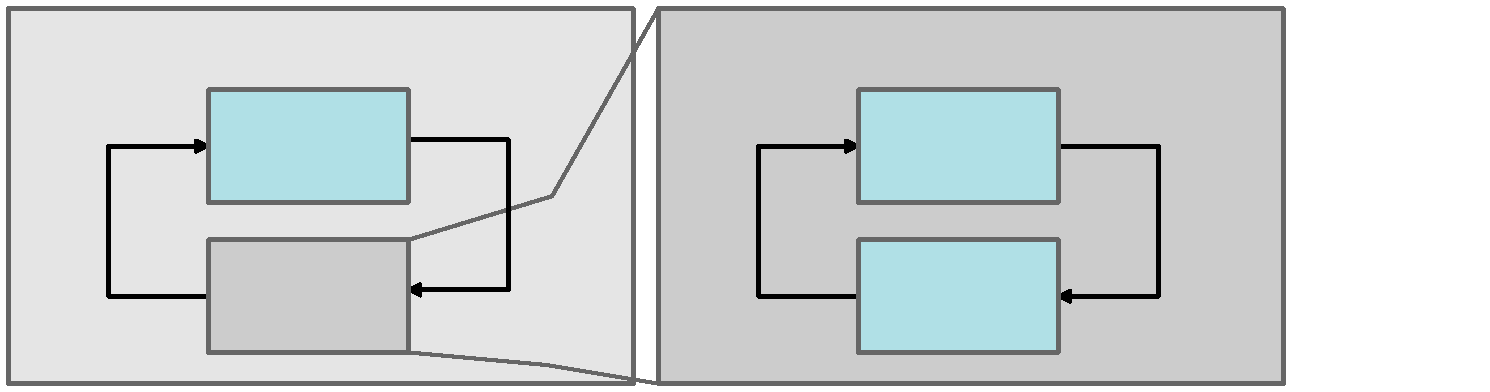
\includegraphics[scale=0.70000]{./figs/optimizer.pdf}\\
   % translate x=1600 y=1120 scale 0.38
   \putbox{3.12900in}{1.64500in}{0.96}{\textbf{B: Optimize $\{K, \omega_z, \omega_p\}$ for fixed $t_{settle}$}}%
   \putbox{4.06700in}{0.97300in}{0.48}{\textbf{to minimize phase noise}}%
   \putbox{4.06700in}{0.56700in}{0.48}{\textbf{Tune parameter $K$}}%
   \putbox{4.06700in}{0.27300in}{0.48}{\textbf{equal to specified value}}%
   \putbox{4.06700in}{0.42000in}{0.48}{\textbf{with GSS to set $t_{settle}$}}%
   \putbox{4.06700in}{1.12000in}{0.48}{\textbf{with gradient descent}}%
   \putbox{4.06700in}{1.26700in}{0.48}{\textbf{Tune parameters $\{\omega_z, \omega_p\}$}}%
   \putbox{3.19200in}{1.47000in}{0.84}{{\color{blue}\texttt{while not converged:}}}%
   \putbox{0.09800in}{1.64500in}{0.96}{\textbf{A: Minimize phase noise subject to $t_{settle,max}$}}%
   \putbox{0.15400in}{1.47000in}{0.84}{{\color{blue}\texttt{while not converged:}}}%
   \putbox{1.02900in}{1.26700in}{0.60}{\textbf{GSS for $t_{settle}$}}%
   \putbox{1.02900in}{1.12000in}{0.48}{\textbf{minimize phase noise}}%
   \putbox{1.02900in}{0.97300in}{0.48}{\textbf{with $0<t_{settle}<t_{settle,max}$}}%
   \putbox{1.02900in}{0.56700in}{0.60}{\textbf{Optimizer B}}%
   \putbox{1.02900in}{0.42000in}{0.48}{\textbf{Minimize phase noise}}%
   \putbox{1.02900in}{0.27300in}{0.48}{\textbf{for fixed $t_{settle}$}}%
   \putbox{1.93200in}{1.23200in}{0.48}{\textbf{current $t_{settle}$}}%
   \putbox{0.35700in}{1.26700in}{0.48}{\textbf{Min. phase noise}}%
   \putbox{5.02600in}{1.20400in}{0.48}{\textbf{$\{K, \omega_z, \omega_p\}$}}%
   \putbox{3.54200in}{1.23200in}{0.48}{\textbf{$\{K, \omega_z, \omega_p\}$}}%
   \putbox{0.35700in}{1.20400in}{0.48}{\textbf{for current $t_{settle}$}}%
   } % close 'parbox'
   } % close 'scalebox'
   \vspace{-\baselineskip} % this is not necessary, but looks better
\fontfamily{\rmdefault}\selectfont

	\caption{Optimizer visualized.}
	\label{fig:optimizer}
\end{figure}

\textbf{Optimizer A - Minimize PLL phase noise given a maximal constraint on settling time.}
\begin{itemize}
	\setlength\itemsep{-0.8em}
	\item Provided a maximum settling time $t_{settle,max}$ and PLL parameters $\{\mathrm{M}$,$\mathrm{N}$,$K_{DCO}$,$S_{0\Phi n_{DCO}}\}$ one-dimensional golden section search (GSS) \cite{press_2007} is used with settling time $t_{settle}$ as the varied parameter, trying to minimize total phase noise power. The cost function for this optimization is the minimum phase noise for each $t_{settle}$ tried found using optimizer B. 
\end{itemize} 
\textbf{Optimizer B - Minimize PLL phase noise for fixed settling time.}\label{lf_opt}
\begin{itemize}
	\setlength\itemsep{-0.8em}
	\item Provided a fixed target for settling time = $t_{settle}$, and PLL parameters $\{\mathrm{M}$,$\mathrm{N}$,$K_{DCO}$,$S_{0\Phi n_{DCO}}\}$, evaluate the two steps, satisfactorily converged of optimization parameters is observed:
	\begin{enumerate}
		\setlength\itemsep{-0.8em}
		\item Minimize total phase noise power using pole/zeros locations $\{\omega_p, \omega_z\}$ using gradient descent with a two-point step size method from \cite{barzilai_borwein_1988}.
		\item Tune $K$ such that settling time is equal to the fixed target value using unconstrained golden section search.
	\end{enumerate}
\end{itemize}

Convergence for gradient descent, GSS and optimizer B algorithms is decided by comparing the parameter values in each optimizer iteration to the previous. If the normalized change in a given iteration for all optimization parameters is below a tolerance specified by the user, convergence is detected and the optimization ends. 

Once the optimal parameters $\{K, \omega_p, \omega_z\}$ for $\mathrm{\hat{T}}(s)$ are determined, the parameter $K$ can be translated onto $K_i$ with equation \ref{eq:map_k_ki}. The loop filter design then can be mapped into a difference equation which is implementable in digital hardware as a a direct form-I IIR architecture, as outlined in section \ref{disc_lf_comp_pi}.
\begin{equation}\label{eq:map_k_ki}
K_i=\frac{\mathrm{M}}{\mathrm{N}}\frac{K}{K_{DCO}}
\end{equation}


\subsection{Fast estimation of PLL settling time}\label{est_set}
	The following is the method implemented to estimate settling time from the PLL closed loop phase transfer function $\mathrm{\hat{T}}(s)$. $\mathrm{\hat{T}}(s)$ can be represented as a rational function of two polynomial functions of s, with P poles and Z zeros. Such a transfer function is computationally represented with arrays A and B, containing the denominator and numerator polynomial coefficients.
	\begin{equation}\label{eq:pll_cl_tf}
	\mathrm{\hat{T}}(s) = \frac{\sum_{j=0}^Z b_js^j}{\sum_{k=0}^P a_ns^n}
	\end{equation}
	An estimate of the step response settling time of $\mathrm{T}(s)$ can by utilizing its representation in state space. This is given in \ref{eq:ss_rep}, with input vector $\mathrm{U}(s)$, state vector $\mathbf{X}(s)$, and output $Y(s)$. The state-space representation from a s-domain transfer function can be quickly solved computationally with available signal processing packages such as \texttt{scipy.signal} \cite{scipy.signal} given the coefficient arrays A and B.
	% https://lpsa.swarthmore.edu/Representations/SysRepTransformations/TF2SS.html
	\begin{align} \label{eq:ss_rep}
		s\mathbf{X}(s) &= \mathbf{AX}(s) +\mathbf{B}\mathrm{U}(s)\\
		Y(s) &= \mathbf{CX}(s) +\mathbf{D}\mathrm{U}(s)
	\end{align}
	The set of k eigenvalues $\{\lambda_1, ... , \lambda_{N}\}$ corresponding to poles for the system are found as the roots of \ref{eq:ss_eigenvals} \cite{brockett_1965}. Matrix $\mathbf{A}$ is referred to as the state matrix.% The associated eigenvectors are found with \ref{eq:ss_eigenvecs}.
	\begin{align}
		|\mathbf{A} - \lambda \mathbf{I}| = 0\label{eq:ss_eigenvals}%\\
		%\mathbf{A} \mathbf{v}_k = \lambda_k\mathbf{v}_k \label{eq:ss_eigenvecs}
	\end{align}
	Imposing the constraint of number of poles P $>$ number of zeros Z, the system $\mathrm{T}(s)$ may be represented via partial fraction decomposition using the poles from the eigenvalues of state matrix $\mathbf{A}$ $\{\lambda_1, ... , \lambda_{N}\}$:
	\begin{equation}
		T(s) = \sum_{k=1}^{P} \frac{c_k}{s-\lambda_k}
	\end{equation}
	Inverse Laplace transformation shows the step response of the system will be a sum of exponentials:
	\begin{equation}
		y(t) = c_1e^{\lambda_1t} + ... + c_ke^{\lambda_kt}%, \hspace{1em} \mathbf{y(t)} = [ y(t) \hspace{0.5em}y^{'}(t)\hspace{0.5em} ...\hspace{0.5em} y^{(k)}(t)]^T
	\end{equation}

	% The state transition matrix $\mathbf{\Phi}_{\mathrm{T}}$ corresponding to the system $\mathrm{T}(s)$ is:
	% \begin{equation}
		% \mathbf{\Phi}_\mathrm{T} = (s\mathbf{I}-A)^{-1}
	% \end{equation}

	The dynamics of the step response are governed by the exponential components of y(t). If  $\{\lambda_1, ... , \lambda_N\} \in \mathds{C}$ where $\lambda_k=1/\tau_k+j\omega_K$, the real portion of each $\lambda_k$ will describe the transient behavior of each exponential, having time constant $\tau_k$. The long term settling of y(t) will be dominated by the exponential with the largest $\tau_k$, i.e. the dominant pole of the system. This estimate of settling time uses the dominant pole $\tau_k$ as a heuristic estimate for overall time constant of the system, $\tau$. Finally, settling time $t_s$ can be considered as the time interval required for the signal to drop within a tolerance band $\pm \delta_{tol} \textnormal{y}(\infty)$ about the final value $\textnormal{y}(\infty)$. Thus:
	\begin{equation}
		t_s = \tau\ln(\delta_{tol}) = \frac{\ln(\delta_{tol})}{\min(|\Re(\{\lambda_1, ... , \lambda_k\})|)}
	\end{equation}
	This settling time estimate is computationally fast, as it requires only (a) computation of state matrix $\mathbf{A}$ from $\mathrm{\hat{T}}(s)$, (b) computation of the eigenvalues of $\mathbf{A}$, and (c) computation of settling time from the eigenvalue with minimum real component.

\subsection{Estimation of PLL phase noise}\label{est_pn}
	The following is the method implemented to estimate total integrated phase noise power from the PLL closed loop phase transfer function $\mathrm{\hat{T}}(s)$, and PLL parameters $\{\mathrm{M}$, $\mathrm{N}$, $K_{DCO}$, $S_{0\Phi n_{DCO}}\}$. As has been stated, this optimizer assumes the dominant output-referred phase noise contributions of the PLL are due to the DCO thermal noise and TDC quantization. If $S_{TDC}$ and $S_{DCO}$ are the PLL output-referred noise PSD respectively for the TDC and DCO noise sources from section \ref{pn_theory}, the total PLL output noise PSD $S_{\Sigma}(f)$ is estimated as \ref{eq:tot_pn_est}.
	\begin{align}\label{eq:tot_pn_est}
		S_{\Sigma}(f) &= S_{\Phi n_{TDC,out}}(f) + S_{\Phi n_{DCO,out}}(f)\\
		 &= \frac{1}{12f_{ref}}\left|2\pi\frac{\mathrm{N}}{\mathrm{M}}\hat{\mathrm{T}}(f)\right|^2 + \frac{S_{0\Phi n_{DCO}}}{f^2}\left|1-\hat{\mathrm{T}}(f)\right|^2
	\end{align}

	Given a bandwidth of interest $\Delta f$ (i.e. baseband bandwidth for radio applications), the total integrated phase noise power is:
	\begin{equation}
		P_{\phi noise} = 2\int_0^{\Delta f} S_{\Sigma}(f)df
	\end{equation}
	This can be computed via numerical integration on a grid of K values in the interval $\Delta f$, where each point represents a frequency bin $f_{bin}$ = $\Delta f$/K. The Romberg method for numerical integration \cite{numerical_methods_2011} is utilized in this work as it has high accuracy for smooth integrands.


\subsection{Loop filter optimization - finite word effects}
Once a filter design has been optimized in the continuous domain following the algorithm of section \ref{lf_opt}, second order optimization is carried out to ensure the digitized, discrete implementation performs as expected in the presence of finite word effects. The optimized digital implementation provided here utilized fixed-point words for equal resolution throughout the datapath. The implemented second order optimization considers both the effect of loop filter quantization noise and transfer function error.

This optimizer works by converting the ideal discrete filter design into a fixed point implementation with direct form-I structure. All components of the data path in the optimization are constrained to have the same signed fixed point format, in twos complement format with 1 sign bit, a number of integer bits \texttt{int\_bits}, and a number of fraction bits \texttt{frac\_bits}. Thus the total data word representation bits is \texttt{B} = 1 + \texttt{int\_bits} + \texttt{frac\_bits}.

Representation of data throughout the digital implementation here

optimum = min number of bits that meets users accuracy and noise spec.

\subsubsection{Loop filter quantization noise optimization}

\begin{figure}[htb!]
	\center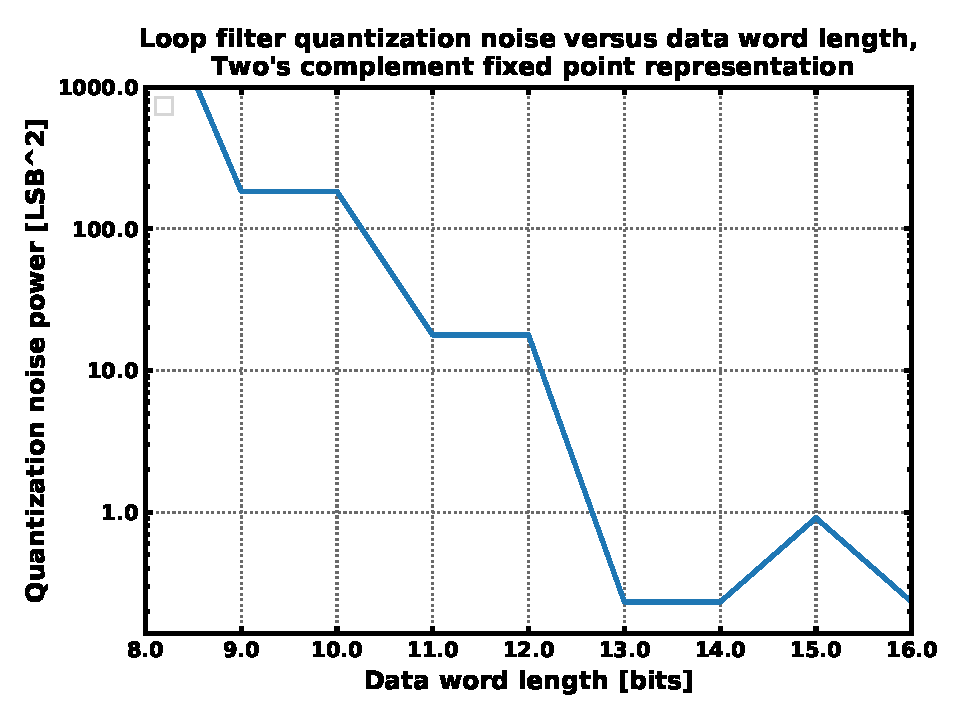
\includegraphics[width=0.5\textwidth, angle=0]{figs/lf_quant_noise.pdf}
	\caption{Quantization noise power power out of an example loop filter versus data word resolution.}
	\label{fig:lf_quant_mse}
\end{figure}


\subsubsection{Loop filter transfer function error optimization}
\begin{figure}[htb!]
    \centering
    \begin{subfigure}{0.5\textwidth}
        \centering
        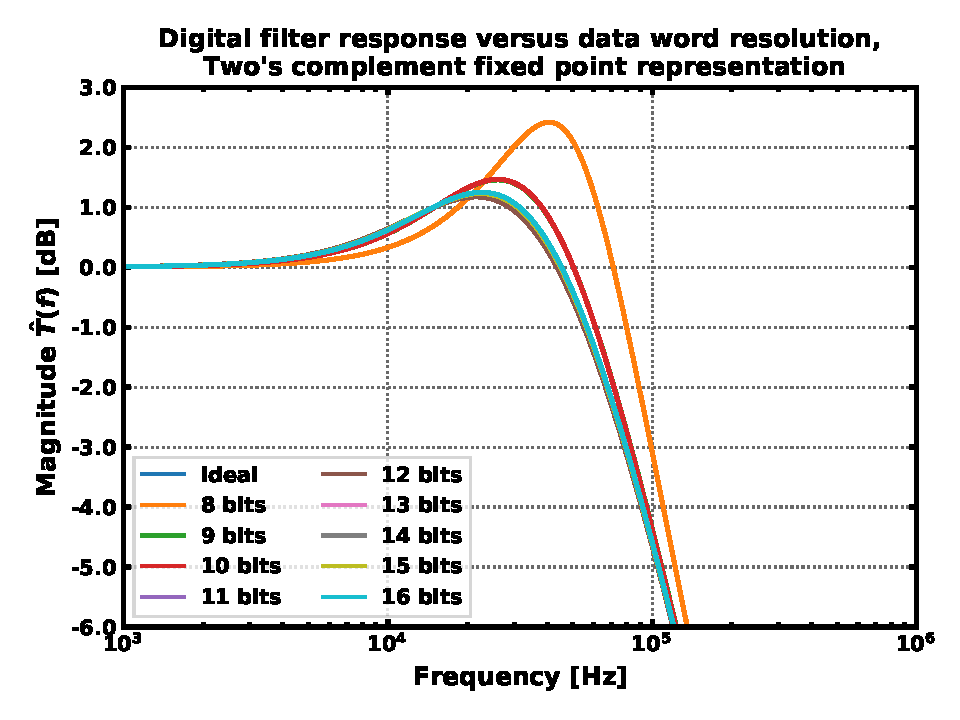
\includegraphics[width=1\textwidth, angle=0]{figs/tf_quant_error.pdf}
        \caption{ }
        \label{fig:tf_curves_quant_error}
    \end{subfigure}%
    \begin{subfigure}{0.5\textwidth}
        \centering
        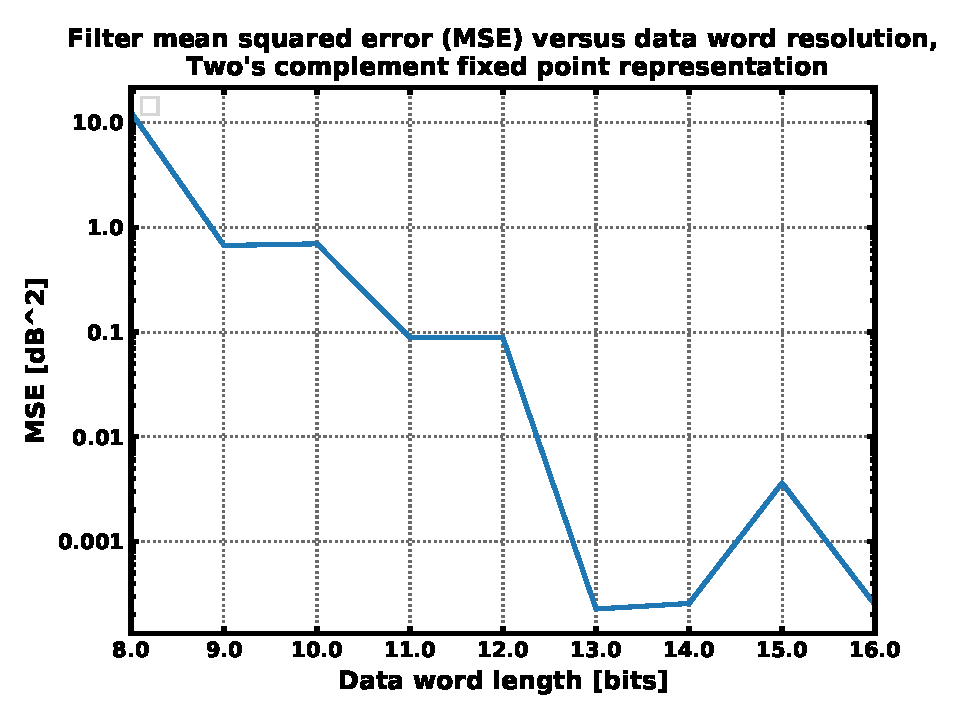
\includegraphics[width=1\textwidth, angle=0]{figs/tf_mse.pdf}
        \caption{ }
        \label{fig:tf_mse}
    \end{subfigure}
    % \caption{Approximate model for ring oscillator inverter delay cell.}
    \label{fig:tf_quant_error}
    \caption{\textbf{(a)} Example filter error due to coefficient quantization, \textbf{(b)} Example MSE error of filter design due to coefficient quantization.}
\end{figure}

    % \section{Results}
    \pagebreak
	\section{Discussion and results}\label{disco}
    %Thus far in this work a solution to simplify and automate design the process of all digital PLL loop filter designs comprised of (1) an automated loop filter optimization and design engine, and (2) a discrete-event, time domain PLL simulator to evaluate the designed filters with full time-discretization and quantization nonlinearity effects. I
In this discussion, the performance of the presented design solution will first be evaluated with a design example. Then, a comparison of the presented solution will be made to existing solutions in literature, pointing out advantages and disadvantages of this work. Finally, a general discussion will be made covering areas of improvement, reasoning for the central design choices made, and considerations for usage the framework.

\subsection{Design Exercise Using This Work}
The design of a loop filter for the PLL with the system level specifications of table \ref{design_specs} will be considered here, with the intent of optimizing total phase noise power (notated in this discussion as residual phase modulation). These specifications, where the TDC resolution in steps equals the divider ratio, is equivalent to a special case of a TDC-less PLL where a 150-step synchronous counter is used as a divider, and the loop filter directly samples the state of the synchronous counter. For the loop filter design, a PI-controller loop filter prototype was utilized in the optimizer due to its predictable phase margin and stability characteristics. Results of two design approaches with this framework will be presented. Approach 1 minimizes the residual phase modulation based on the TDC-phase detector PLL model. The BBPD gain in this case is optimized to minimize phase noise spectrum error in steady state for that expected from the TDC-PLL model. Approach 2 demonstrates loop filter optimization for both fast locking and low phase noise using loop filter gear switching. The first gear loop filter is optimized for minimum lock time using TDC feedback, and the second gear is optimized to minimize residual phase modulation in steady state using BBPD feedback.

% \scriptsize
\begin{table}[h!]
	\centering
	\def\arraystretch{1.5}		
	\setlength\arrayrulewidth{0.75pt}
	\setlength{\tabcolsep}{1em} % for the horizontal padding
	\begin{tabular}{|l|r|l|}
		\hline 
		\rule[-1ex]{0pt}{2.5ex} \cellcolor{gray!40}\textbf{Parameter} & \cellcolor{gray!40}\textbf{Value} & \cellcolor{gray!40}\textbf{Unit }\\ 
		\hline 
		\rule[-1ex]{0pt}{2.5ex} \textbf{Output Frequency}  & 2.4 & GHz \\ 
		\hline 
		\rule[-1ex]{0pt}{2.5ex} \textbf{Ref. frequency} & 16 & MHz\\ 
		\hline 
		\rule[-1ex]{0pt}{2.5ex} \textbf{Divider ratio} & 150  &\\ 
		\hline 
		\rule[-1ex]{0pt}{2.5ex} \textbf{TDC resolution} & 150  & steps/reference cycle\\ 
		\hline 
		\rule[-1ex]{0pt}{2.5ex} \textbf{DCO gain $K_{DCO}$} & $10^4$ & Hz/LSB \\ 
		\hline 
		\rule[-1ex]{0pt}{2.5ex} \textbf{DCO Phase noise} & -80 & dBc/Hz at $\Delta f=10^6$ Hz \\ 
		\hline 
		\rule[-1ex]{0pt}{2.5ex} \textbf{Lock Time} & $\leq$ 25 & $\mu$s \\ 
		\hline 
		\rule[-1ex]{0pt}{2.5ex} \textbf{Lock $\Delta f$ tolerance} & $10^5$ & Hz \\ 
		\hline 
		\rule[-1ex]{0pt}{2.5ex} \textbf{Digital filter word resolution} & $\leq$ 16 & bits \\ 
		\hline 
		\rule[-1ex]{0pt}{2.5ex} \textbf{Residual phase modulation} & minimize &  \\ 
		\hline 
	\end{tabular} 
	% \caption{Assigned specifications for branch line hybrid design.}
	% \label{asgn_specs}
	\caption{System-level specifications}
	\label{design_specs}
\end{table}   

\subsubsection{Approach 1: Results of Filter Optimization.}
Table \ref{filter_params} contains the optimized filter parameters obtained from the filter design optimizer developed in this work using the TDC based PLL model. $\{K$, $K_i$, $K_p$, $f_z\}$ are the continuous model parameters of section \ref{cont_pi_filt_des}, and $\{a_0$, $a_1$, $a_2$, $b_0$, $b_1\}$ are the filter coefficients for the discrete-time direct form-I filter structure of section \ref{disc_lf_comp_pi}. The estimated bandwidth for the filter is 144.8 kHz, and the lock time is estimated to be 19.3 $\mu$s. Table \ref{dig_filter_params} contains the digitized version of the discrete time filter, based on a selection for word size determined via optimization for finite word effects. The final data words are 13 bits in length.  
% \scriptsize
\begin{table}[h!]
	\centering
	\def\arraystretch{1.5}		
	\setlength\arrayrulewidth{0.75pt}
	\setlength{\tabcolsep}{1em} % for the horizontal padding
	\begin{tabular}{|l|r|l|}
		\hline 
		\rule[-1ex]{0pt}{2.5ex} \cellcolor{gray!40}\textbf{Parameter} & \cellcolor{gray!40}\textbf{Value} & \cellcolor{gray!40}\textbf{Unit }\\ 
		\hline 
		\rule[-1ex]{0pt}{2.5ex} \textbf{$K$}  & $1.343792\times10^{11}$ &  \\ 
		\hline 
		\rule[-1ex]{0pt}{2.5ex} \textbf{$K_i$}  & $1.343792\times10^{7}$ &  \\ 
		\hline 
		\rule[-1ex]{0pt}{2.5ex} \textbf{$K_p$}  & $7.331074\times10^{1}$ &  \\ 
		\hline 
		\rule[-1ex]{0pt}{2.5ex} \textbf{$f_z$} & $2.917324\times10^4$ & Hz\\ 
		\hline 
		\rule[-1ex]{0pt}{2.5ex} \textbf{$b_0$}  & $7.4150613906\times10^1$  &\\ 
		\hline 
		\rule[-1ex]{0pt}{2.5ex} \textbf{$b_1$}  & $-7.3310743796\times10^1$  & \\ 
		\hline 
		\rule[-1ex]{0pt}{2.5ex} \textbf{$a_0$}  & $1.0\times10^0$  &\\ 
		\hline 
		\rule[-1ex]{0pt}{2.5ex} \textbf{$a_1$}  & $-1.0\times10^0$  & \\ 
		\hline 
		\rule[-1ex]{0pt}{2.5ex} \textbf{$a_2$}  & $0.0\times10^0$  & \\ 
		\hline 
		\rule[-1ex]{0pt}{2.5ex} \textbf{$K_{bb}$}  & $3.007953\times10^{-2}$  & \\ 
		\hline 
		\rule[-1ex]{0pt}{2.5ex} Estimated bandwidth & $1.448234\times10^5$ & Hz \\ 
		\hline 
		\rule[-1ex]{0pt}{2.5ex} Estimated lock time & $1.934253\times10^{-5}$ & seconds \\ 
		\hline 
	\end{tabular} 
	% \caption{Assigned specifications for branch line hybrid design.}
	% \label{asgn_specs}
	\caption{PLL parameters determined from filter design and optimization process.}
	\label{filter_params}
\end{table}   

\begin{table}[h!]
	\centering
	\def\arraystretch{1.5}		
	\setlength\arrayrulewidth{0.75pt}
	\setlength{\tabcolsep}{1em} % for the horizontal padding
	\begin{tabular}{|l|r|r|l|}
		\hline 
		\rule[-1ex]{0pt}{2.5ex} \cellcolor{gray!40}\textbf{Parameter} & \cellcolor{gray!40}\textbf{Value} & \cellcolor{gray!40}\textbf{Value (digital) } & \cellcolor{gray!40}\textbf{Value Error}\\ 
		\hline 
		\rule[-1ex]{0pt}{2.5ex} Total dataword bits  & 13 & & \\ 
		\hline 
		\rule[-1ex]{0pt}{2.5ex} Sign bits  & 1 & & \\ 
		\hline 
		\rule[-1ex]{0pt}{2.5ex} Integer bits & 7 & & \\ 
		\hline 
		\rule[-1ex]{0pt}{2.5ex} Fractional bits  & 5 & & \\ 
		\hline 
		\rule[-1ex]{0pt}{2.5ex} \textbf{$b_0$} & $7.415625\times10^1$ & \texttt{0b0100101000101}  & $+5.636094\times10^{-3}$\\ 
		\hline 
		\rule[-1ex]{0pt}{2.5ex} \textbf{$b_1$}  & $-7.331250\times10^1$ & \texttt{0b1111011010110}  & $-1.756204\times10^{-3}$\\ 
		\hline 
		\rule[-1ex]{0pt}{2.5ex} \textbf{$a_0$}  & $1.0\times10^0$ & \texttt{0b0000000100000} & $0.0\times10^0$ \\ 
		\hline 
		\rule[-1ex]{0pt}{2.5ex} \textbf{$a_1$}  & $-1.0\times10^0$ & \texttt{0b1111111100000} & $0.0\times10^0$ \\ 
		\hline 
		\rule[-1ex]{0pt}{2.5ex} \textbf{$a_2$}  & $0.0\times10^0$ & \texttt{0b0000000000000} & $0.0\times10^0$ \\ 
		\hline 
		\rule[-1ex]{0pt}{2.5ex} \textbf{$K_{bb}$}  & $3.125\times10^{-2}$ & \texttt{0b0000000000001} & $+1.170461\times10^-3$ \\ 
		\hline 
	\end{tabular} 
	% \caption{Assigned specifications for branch line hybrid design.}
	% \label{asgn_specs}
	\caption{Loop filter parameters after digitization and optimization for data word length.}
	\label{dig_filter_params}
\end{table}  
\pagebreak

\subsubsection{Approach 1: Results of Transient and Phase Noise Simulation.}
The simulation engine implemented in this work was utilized to run a time domain simulation to verify the designed filter. Figures \ref{fig:trans_lf} and \ref{fig:trans_inst_freq} demonstrate the transient response of the PLL with an initial frequency error of 12 MHz (0.5\% of final frequency). It is observed that the PLL design stably approaches the target frequency in approximately 23 $\mu$s. Figures \ref{fig:trans_det} illustrate the BBPD and TDC outputs during this initial transient. It is observed that the TDC output gives the dominant feedback, until it reaches an output word of 0, where the BBPD then begins providing feedback in the steady state condition of the PLL. Figure \ref{fig:trans_phase_noise} is the result of a phase noise calculation for the simulated PLL in an interval beginning immediately after detection of lock. The spectrum closely approximates that designed for, with some small additional peaking.
	\begin{figure}[htb!]
	    \centering
	    \begin{subfigure}{0.5\textwidth}
	        \centering
	        \center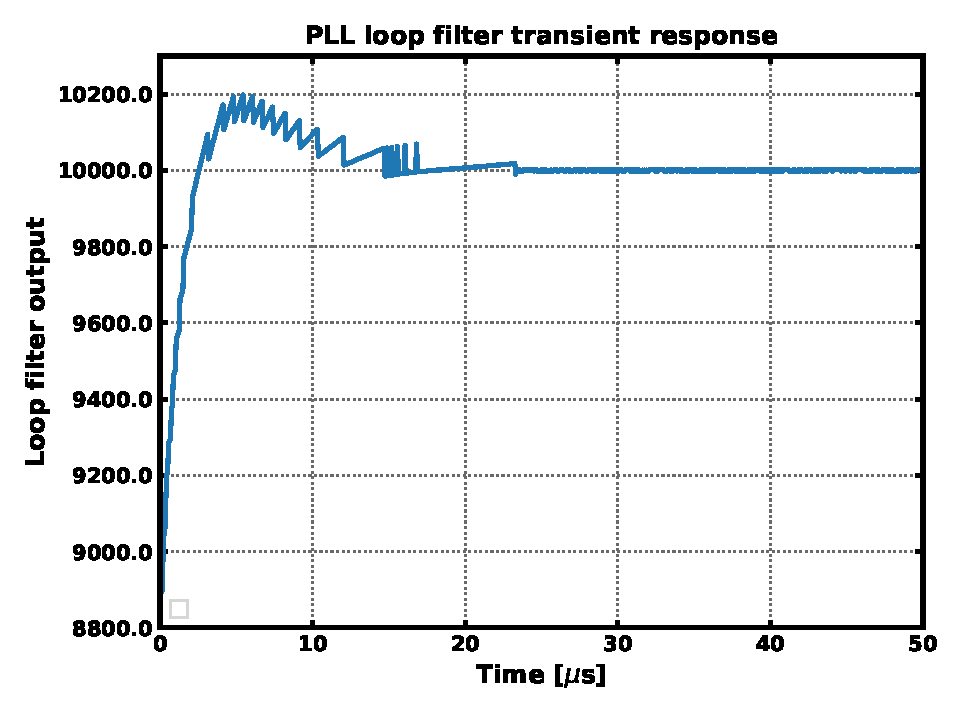
\includegraphics[width=1.0\textwidth, angle=0]{figs/trans_loop_filter.pdf}
	        \caption{ }
	        \label{fig:trans_lf}
	    \end{subfigure}%
	    \begin{subfigure}{0.5\textwidth}
	        \centering
	        \center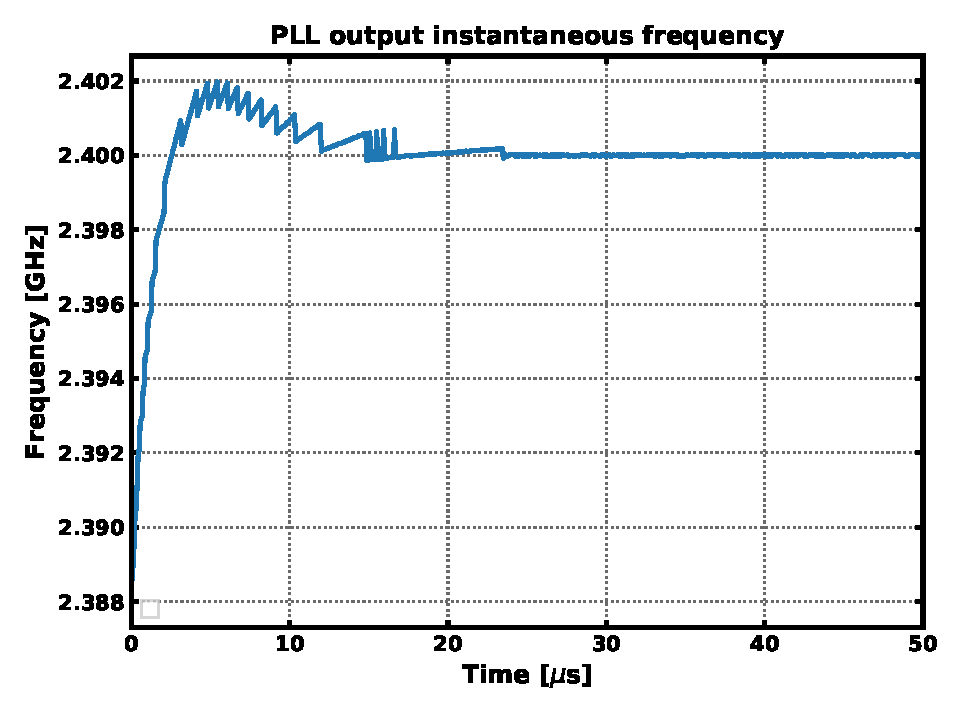
\includegraphics[width=1.0\textwidth, angle=0]{figs/trans_inst_freq.pdf}
	        \caption{ }
	        \label{fig:trans_inst_freq}
	    \end{subfigure}
	    % \caption{Approximate model for ring oscillator inverter delay cell.}
	    \label{fig:trans_sim1}
	    \caption{Simulation with 0.5\% initial frequency error: \textbf{(a)} Loop filter transient response, \textbf{(b)} PLL output instantaneous frequency.}
	\end{figure}

	\begin{figure}[htb!]
	    \centering
	    \begin{subfigure}{0.5\textwidth}
	        \centering
	        \center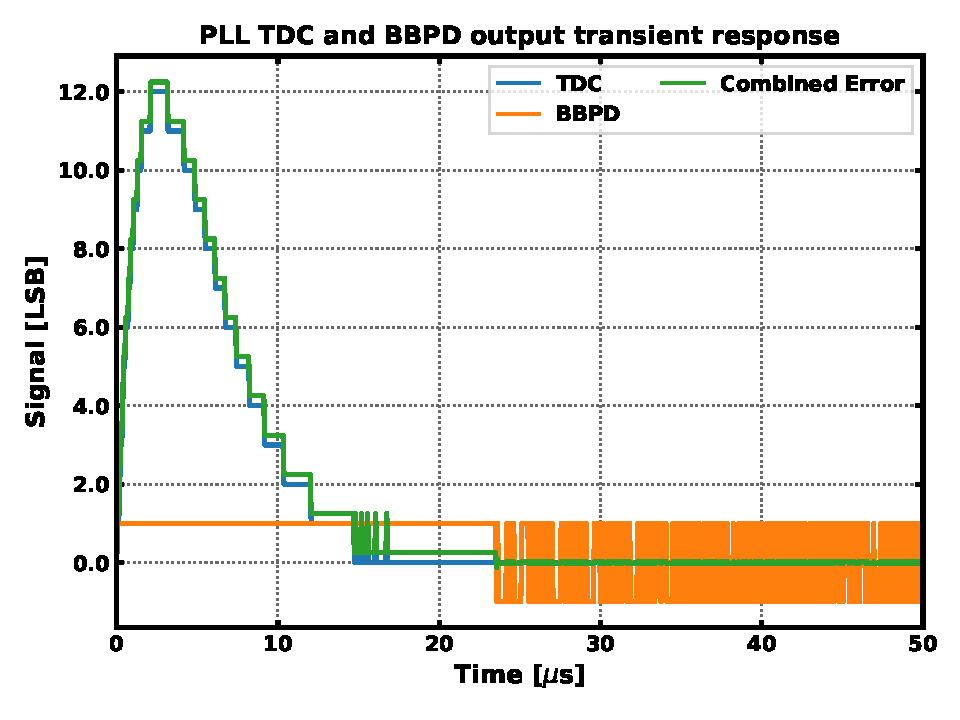
\includegraphics[width=1.0\textwidth, angle=0]{figs/trans_tdc_bbpd.pdf}
	        \caption{ }
	        \label{fig:trans_det}
	    \end{subfigure}%
	    \begin{subfigure}{0.5\textwidth}
	        \centering
	        \center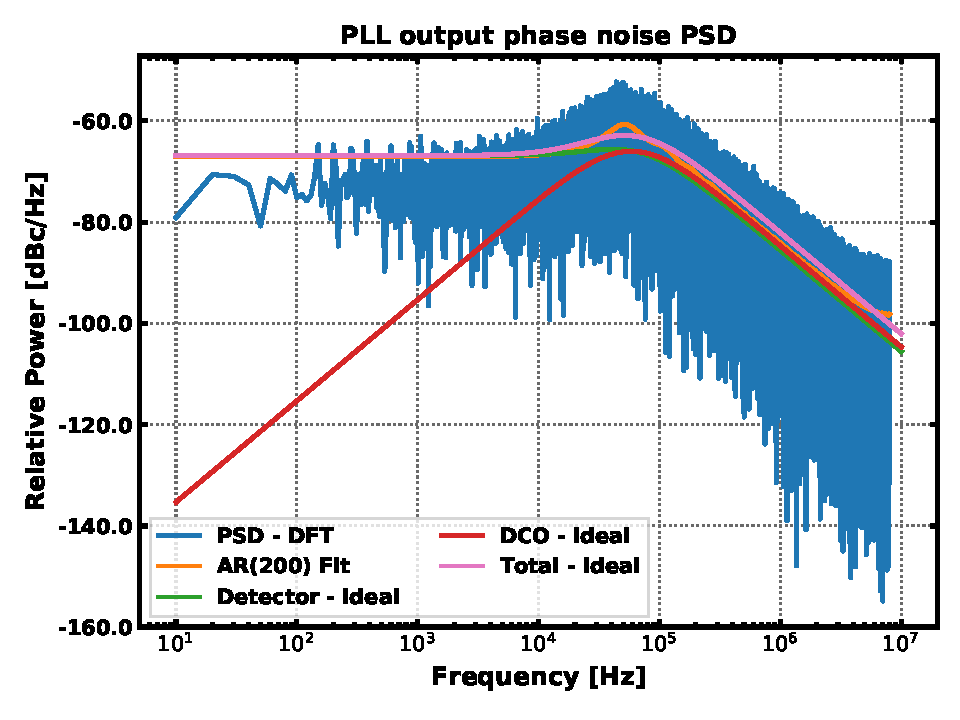
\includegraphics[width=1.0\textwidth, angle=0]{figs/trans_phase_noise.pdf}
	        \caption{ }
	        \label{fig:trans_phase_noise}
	    \end{subfigure}
	    % \caption{Approximate model for ring oscillator inverter delay cell.}
	    \label{fig:trans_sim2}
	    \caption{Simulation with 12 MHz (0.5\%) initial frequency error: \textbf{(a)} BBPD/TDC detector responses, \textbf{(b)} PLL output phase noise power spectrum.}
	\end{figure}
\pagebreak

\subsubsection{Approach 1: Results of Parameter Sweep and Variational Analysis.}
The Monte-Carlo sampling and parametric sweep capabilities of the simulator designed in this work were used to run analysis for effects of variation of DCO gain $K_{DCO}$ and initial frequency error of the PLL. Figure \ref{fig:sweep_kdco} shows a parametric sweep of $K_{DCO}$, with lock time being measured. It is observed that the lock time is nearly flat in the range 7100-21200 Hz/LSB, meaning that there is a tolerance of -2900/+11200 Hz LSB for $K_{DCO}$ about the nominal 10000 Hz/LSB specified. This specification can be utilized in the design of a physical DCO to constrain maximum acceptable variation across PVT. Figure \ref{fig:sweep_finit} demonstrates the simulated effect of initial frequency error on lock time. It is seen that PLL stably locks to the target frequency with an initial frequency error within the interval of $\pm$ 74 MHz from 2.4GHz, implying that the capture range of the PLL is 148 MHz. This specification can be translated into a requirement for initial coarse frequency calibration needed before starting the PLL. Figures \ref{fig:mc_trans} and \ref{fig:mc_hist} are the results of a variation analysis simulation utilizing the Monte-Carlo sampling engine implemented in this work. The simulation was configured to vary $K_{DCO}$ with a standard deviation of 20 \% of the nominal value, and to vary the initial starting frequency with a standard deviation of 60 MHz (2.5 \% of the final frequency). The simulation sample size is 1000. The transient responses from the simulation figure \ref{fig:mc_trans} are all stable, and figure \ref{fig:mc_hist} shows the histogram for measured lock time subject to the described variation. The mean lock time was 19.33 $\mu$s, which correlates well with the estimated 19.34 $\mu$s from the filter design process and meets the 25 $\mu$s lock time set for the PLL. The upper bound for a 99\% confidence interval on the data is 34.75 $\mu$s. A set of extracted parameters from these simulations are in table \ref{simulation_params}. The Monte-Carlo simulations presented here are useful to analyze the range of variation in which the designed PLL can tolerate, as well as determine the expected performance variation, so well informed decisions on a PLL design can be made before moving into transistor level implementation and simulation. 

	\begin{figure}[htb!]
	    \centering
	    \begin{subfigure}{0.5\textwidth}
	        \centering
	        \center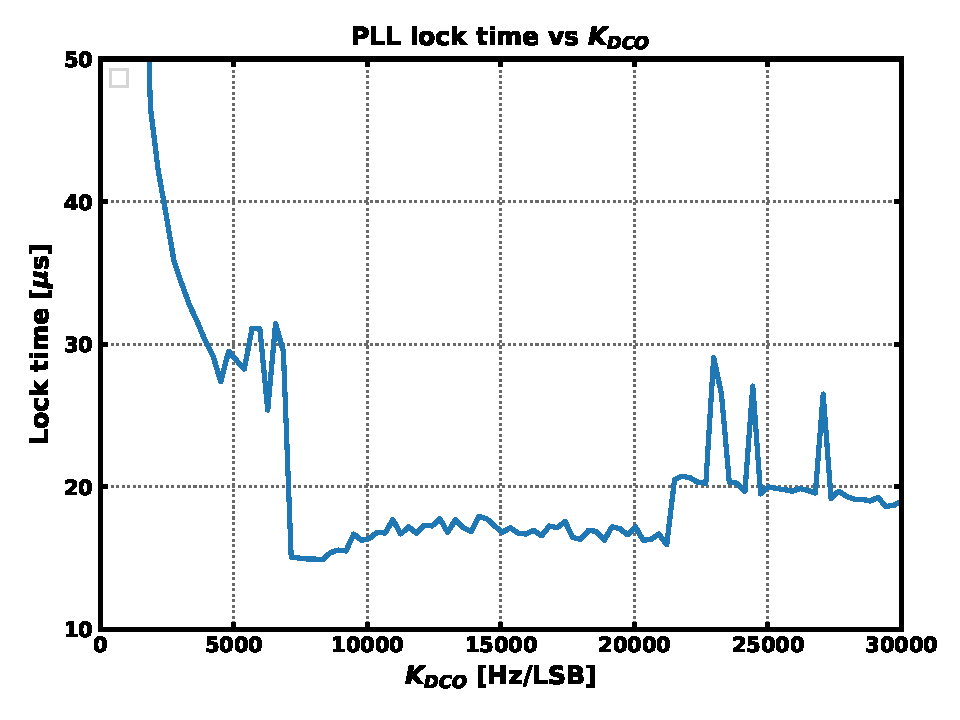
\includegraphics[width=1.0\textwidth, angle=0]{figs/_kdco_sweep.pdf}
	        \caption{ }
	        \label{fig:sweep_kdco}
	    \end{subfigure}%
	    \begin{subfigure}{0.5\textwidth}
	        \centering
	        \center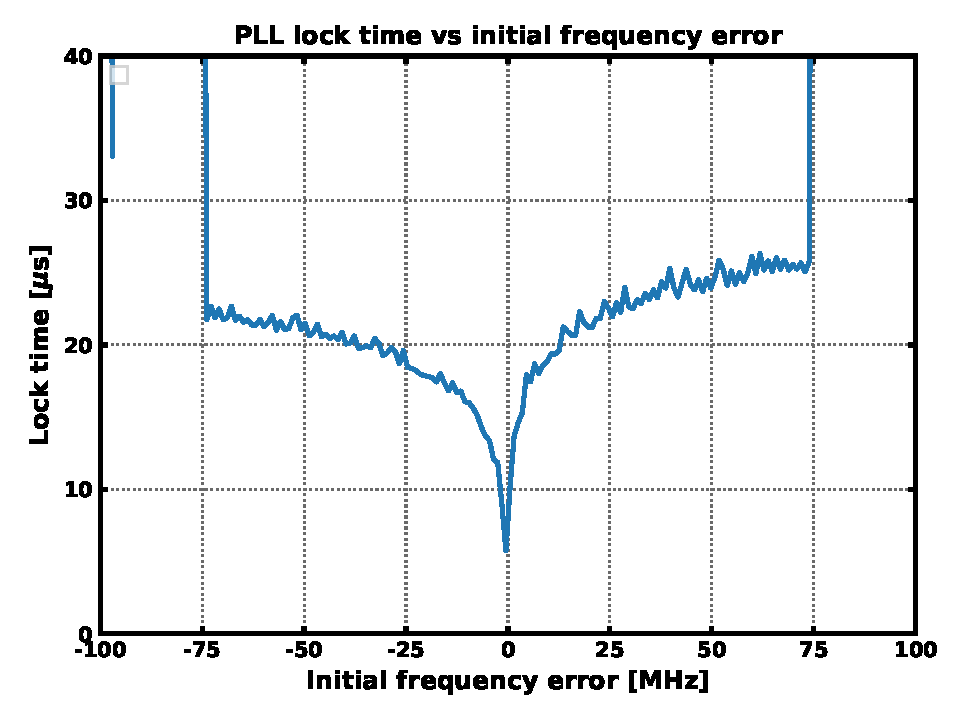
\includegraphics[width=1.0\textwidth, angle=0]{figs/_finit_sweep.pdf}
	        \caption{ }
	        \label{fig:sweep_finit}
	    \end{subfigure}
	    % \caption{Approximate model for ring oscillator inverter delay cell.}
	    \label{fig:sweep_sim}
	    \caption{\textbf{(a)} PLL lock time simulation with KDCO swept, 12 MHz (0.5\%) initial frequency error, \textbf{(b)} PLL lock time simulation with initial frequency error swept.}
	\end{figure}

	\begin{figure}[htb!]
	    \centering
	    \begin{subfigure}{0.5\textwidth}
	        \centering
	        \center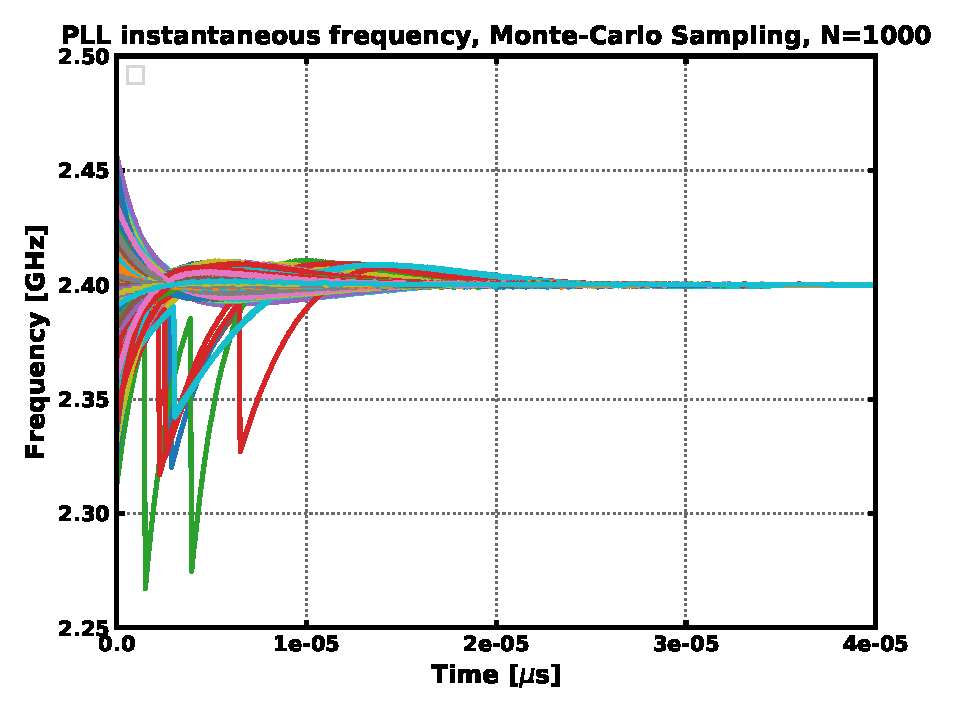
\includegraphics[width=1.0\textwidth, angle=0]{figs/mc_trans.pdf}
	        \caption{ }
	        \label{fig:mc_trans}
	    \end{subfigure}%
	    \begin{subfigure}{0.5\textwidth}
	        \centering
	        \center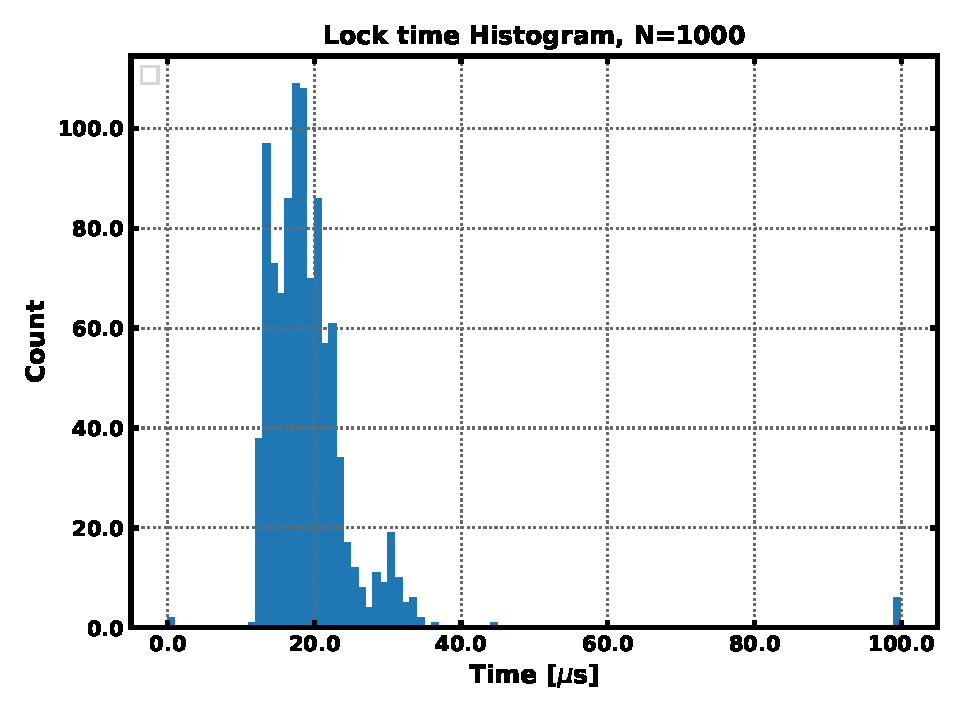
\includegraphics[width=1.0\textwidth, angle=0]{figs/mc_hist.pdf}
	        \caption{ }
	        \label{fig:mc_hist}
	    \end{subfigure}
	    % \caption{Approximate model for ring oscillator inverter delay cell.}
	    \label{fig:mc_sim}
	    \caption{Monte-Carlo simulation with 1000 samples, 20\% RMS deviation in KDCO, and 60 MHz (2.5\%) RMS deviation in initial frequency error \textbf{(a)} Frequency transient responses, \textbf{(b)} Lock time histogram.}
	\end{figure}

\begin{table}[h!]
	\centering
	\def\arraystretch{1.5}		
	\setlength\arrayrulewidth{0.75pt}
	\setlength{\tabcolsep}{1em} % for the horizontal padding
	\begin{tabular}{|l|r|l|}
		\hline 
		\rule[-1ex]{0pt}{2.5ex} \cellcolor{gray!40}\textbf{Parameter} & \cellcolor{gray!40}\textbf{Value} & \cellcolor{gray!40}\textbf{Unit }\\ 
		\hline 
		\rule[-1ex]{0pt}{2.5ex} \textbf{$K_{DCO}$ Tolerance}  & -2900/+11200 & Hz/LSB \\ 
		\hline 
		\rule[-1ex]{0pt}{2.5ex} \textbf{Capture range}  & 148 ($\pm 74$)& MHz\\ 
		\hline 
		\rule[-1ex]{0pt}{2.5ex} \textbf{Mean lock time}  & 19.32769& $\mu$s \\ 
		\hline 
		\rule[-1ex]{0pt}{2.5ex} \textbf{Lock time $\sigma$} & 7.802302 & $\mu$s\\ 
		\hline 
		\rule[-1ex]{0pt}{2.5ex} \textbf{Lock time 99 \% CI upper bound} & 34.75  & $\mu$s\\ 
		\hline 
		\rule[-1ex]{0pt}{2.5ex} \textbf{Residual phase modulation} & $3.374731\times10^{-1}$  & rad$^2$\\ 
		\hline 
	\end{tabular} 

	% \caption{Assigned specifications for branch line hybrid design.}
	% \label{asgn_specs}
	\caption{PLL parameters extracted from variance and parameter sweep simulations.}
	\label{simulation_params}
\end{table}

\subsubsection{Approach 2: Results of Filter Optimization}
The same PLL design has been approached with a second optimization approach utilizing gear switching in the loop filter. The first gear loop filter is optimized for lock speed, using TDC feedback, so high initial frequency and phase errors may be tolerated. After initial lock is achieved with the first filter, the filter is switched gears by changing the digital filter coefficients immediately to a second filter optimized for minimum total phase noise using a BBPD. This combination allow both fast lock and low phase noise. The results of the optimization process are in tables \ref{filter_params_fast_lock} and \ref{filter_params_bbpd_low_noise}, and the optimal digitized filter designs for finite word effects are in table \ref{dig_filter_params_fast}. The total lock time is estimated to be 5.52 $\mu$s. The method for determining number of bits in this work currently assumes the decimal point in the fixed point representation does not change position, so here a total data word size of 20 bits was arrived at, albeit the individual optimization for gear 1 and gear 2 resulted in 10 and 16 bits respectively. This optimization could be improved by considering a filter datapath architecture that handles changing of the decimal position in the loop filter data words during gear switching.

\begin{table}[h!]
	\centering
	\def\arraystretch{1.5}		
	\setlength\arrayrulewidth{0.75pt}
	\setlength{\tabcolsep}{1em} % for the horizontal padding
	\begin{tabular}{|l|r|l|}
		\hline 
		\rule[-1ex]{0pt}{2.5ex} \cellcolor{gray!40}\textbf{Parameter} & \cellcolor{gray!40}\textbf{Value} & \cellcolor{gray!40}\textbf{Unit }\\ 
		\hline 
		\rule[-1ex]{0pt}{2.5ex} \textbf{$K$}  & $2.982197\times10^{12}$ &  \\
		\hline 
		\rule[-1ex]{0pt}{2.5ex} \textbf{$K_i$}  & $2.982197\times10^{8}$ &  \\
		\hline 
		\rule[-1ex]{0pt}{2.5ex} \textbf{$K_p$}  & $2.115052\times10^{2}$ &  \\
		\hline 
		\rule[-1ex]{0pt}{2.5ex} \textbf{$f_z$} & $2.244064\times10^5$ & Hz\\
		\hline 
		\rule[-1ex]{0pt}{2.5ex} \textbf{$b_0$}  & $2.3014397180\times10^2$  &\\
		\hline 
		\rule[-1ex]{0pt}{2.5ex} \textbf{$b_1$}  & $-2.1150524223\times10^2$  & \\
		\hline 
		\rule[-1ex]{0pt}{2.5ex} \textbf{$a_0$}  & $1.0\times10^0$  &\\ 
		\hline 
		\rule[-1ex]{0pt}{2.5ex} \textbf{$a_1$}  & $-1.0\times10^0$  & \\
		\hline 
		\rule[-1ex]{0pt}{2.5ex} \textbf{$a_2$}  & $0.0\times10^0$  & \\
		\hline 
		\rule[-1ex]{0pt}{2.5ex} Estimated bandwidth & $5.333423\times10^5$ & Hz \\
		\hline 
		\rule[-1ex]{0pt}{2.5ex} Estimated lock time & $4.527067\times10^{-6}$ & seconds \\
		\hline 
	\end{tabular} 
	% \caption{Assigned specifications for branch line hybrid design.}
	% \label{asgn_specs}
	\caption{PLL parameters determined from filter design and optimization process for fast lock speed with TDC feedback.}
	\label{filter_params_fast_lock}
\end{table}   

\begin{table}[h!]
	\centering
	\def\arraystretch{1.5}		
	\setlength\arrayrulewidth{0.75pt}
	\setlength{\tabcolsep}{1em} % for the horizontal padding
	\begin{tabular}{|l|r|l|}
		\hline 
		\rule[-1ex]{0pt}{2.5ex} \cellcolor{gray!40}\textbf{Parameter} & \cellcolor{gray!40}\textbf{Value} & \cellcolor{gray!40}\textbf{Unit }\\ 
		\hline 
		\rule[-1ex]{0pt}{2.5ex} \textbf{$K$}  & $5.325862\times12^{12}$ &  \\
		\hline 
		\rule[-1ex]{0pt}{2.5ex} \textbf{$K_i$}  & $1.271456\times10^{10}$ &  \\
		\hline 
		\rule[-1ex]{0pt}{2.5ex} \textbf{$K_p$}  & $1.101813\times10^{4}$ &  \\
		\hline 
		\rule[-1ex]{0pt}{2.5ex} \textbf{$f_z$} & $1.836596\times10^5$ & Hz\\
		\hline 
		\rule[-1ex]{0pt}{2.5ex} \textbf{$b_0$}  & $1.1812790734\times10^4$  &\\
		\hline 
		\rule[-1ex]{0pt}{2.5ex} \textbf{$b_1$}  & $-1.1018130778\times10^4$  & \\
		\hline 
		\rule[-1ex]{0pt}{2.5ex} \textbf{$a_0$}  & $1.0\times10^0$  &\\ 
		\hline 
		\rule[-1ex]{0pt}{2.5ex} \textbf{$a_1$}  & $-1.0\times10^0$  & \\ 
		\hline 
		\rule[-1ex]{0pt}{2.5ex} \textbf{$a_2$}  & $0.0\times10^0$  & \\ 
		\hline 
		\rule[-1ex]{0pt}{2.5ex} \textbf{$K_{bb}$}  & $1.0\times10^0$  & \\ 
		\hline 
		\rule[-1ex]{0pt}{2.5ex} Estimated bandwidth & $9.117332\times10^5$ & Hz \\
		\hline 
		\rule[-1ex]{0pt}{2.5ex} Estimated lock time & $9.978130\times10^{-7}$ & seconds \\
		\hline 
	\end{tabular} 
	% \caption{Assigned specifications for branch line hybrid design.}
	% \label{asgn_specs}
	\caption{PLL parameters determined from filter design and optimization process for minimum phase noise with BBPD.}
	\label{filter_params_bbpd_low_noise}
\end{table}   

\begin{table}[h!]
	\centering
	\def\arraystretch{1.5}		
	\setlength\arrayrulewidth{0.75pt}
	\setlength{\tabcolsep}{1em} % for the horizontal padding
	\begin{tabular}{|l|r|r|l|}
		\hline 
		\rule[-1ex]{0pt}{2.5ex} \cellcolor{gray!40}\textbf{Parameter} & \cellcolor{gray!40}\textbf{Value} & \cellcolor{gray!40}\textbf{Value (digital) } & \cellcolor{gray!40}\textbf{Value Error}\\ 
		\hline 
		\rule[-1ex]{0pt}{2.5ex} Total dataword bits  & 20 & & \\ 
		\hline 
		\rule[-1ex]{0pt}{2.5ex} Sign bits  & 1 & & \\ 
		\hline 
		\rule[-1ex]{0pt}{2.5ex} Integer bits & 8 & & \\ 
		\hline 
		\rule[-1ex]{0pt}{2.5ex} Fractional bits  & 11 & & \\ 
		\hline 
		\rule[-1ex]{0pt}{2.5ex} \textbf{$b_0$} {\color{red} (gear 1)} & $2.301440\times10^2$ & \texttt{0b01110011000100100111}  & $+7.116930\times10^{-5}$\\
		\hline 
		\rule[-1ex]{0pt}{2.5ex} \textbf{$b_1$} {\color{red} (gear 1)} & $-2.115054\times10^2$ & \texttt{0b11110110001111110101}  & $-1.288619\times10^{-4}$\\
		\hline 
		\rule[-1ex]{0pt}{2.5ex} \textbf{$a_0$} {\color{red} (gear 1)} & $1.0\times10^0$ & \texttt{0b00000000100000000000} & $0.0\times10^0$ \\ 
		\hline 
		\rule[-1ex]{0pt}{2.5ex} \textbf{$a_1$} {\color{red} (gear 1)} & $-1.0\times10^0$ & \texttt{0b11111111100000000000} & $0.0\times10^0$ \\ 
		\hline 
		\rule[-1ex]{0pt}{2.5ex} \textbf{$a_2$} {\color{red} (gear 1)} & $0.0\times10^0$ & \texttt{0b00000000000000000000} & $0.0\times10^0$ \\ 
		\hline 
		\rule[-1ex]{0pt}{2.5ex} \textbf{$K_{bb}$} {\color{red} (gear 1)} & $0.0\times10^0$ & \texttt{0b00000000000000000000} & $0.0\times10^0$ \\ 
		\hline 
		\rule[-1ex]{0pt}{2.5ex} \textbf{$b_0$} {\color{blue} (gear 2)} & $8.899902\times10^0$ & \texttt{0b00000100011100110011}  & $+4.616306\times10^{-5}$\\
		\hline 
		\rule[-1ex]{0pt}{2.5ex} \textbf{$b_1$} {\color{blue} (gear 2)} & $-8.301270\times10^0$ & \texttt{0b11111011110110010111}  & $-1.168639\times10^{-4}$\\
		\hline 
		\rule[-1ex]{0pt}{2.5ex} \textbf{$a_0$} {\color{blue} (gear 2)} & $1.0\times10^0$ & \texttt{0b00000000100000000000} & $0.0\times10^0$ \\ 
		\hline 
		\rule[-1ex]{0pt}{2.5ex} \textbf{$a_1$} {\color{blue} (gear 2)} & $-1.0\times10^0$ & \texttt{0b11111111100000000000} & $0.0\times10^0$ \\ 
		\hline 
		\rule[-1ex]{0pt}{2.5ex} \textbf{$a_2$} {\color{blue} (gear 2)} & $0.0\times10^0$ & \texttt{0b00000000000000000000} & $0.0\times10^0$ \\ 
		\hline 
		\rule[-1ex]{0pt}{2.5ex} \textbf{$K_{bb}$} {\color{blue} (gear 2)} & $1.0\times10^0$ & \texttt{0b00000000100000000000} & $1\times10^0$ \\ 
		\hline 
	\end{tabular} 
	% \caption{Assigned specifications for branch line hybrid design.}
	% \label{asgn_specs}
	\caption{Loop filter parameters after digitization and optimization for data word length, gear 1 and gear 2.}
	\label{dig_filter_params_fast}
\end{table}  

\subsubsection{Approach 2: Results of Transient and Phase Noise Simulation}
It is observed that the fast lock gear converges the PLL to steady state in approximately 6 $\mu$s as seen in the transient step simulation in figures \ref{fig:trans_lf_fast} and \ref{fig:trans_inst_freq_fast}, where an initial frequency error of 0.5\% {12 MHz} is used. Figure \ref{fig:trans_det_fast} shows the output of the TDC and BBPD, it is seen that BBPD feedback has a high density at approximately 11 $\mu$s, implicating steady state conditions. Finally, the computed phase noise spectrum of figure \ref{fig:trans_phase_noise_fast} demonstrates that there is some discrepancy between the ideal designed response and that simulated, albeit the bandwidth appears correct. The phase noise spectrum discrepancy is likely due to the model used in the optimization for the BBPD, which uses a linearized model of the BBPD with only idealized DCO and detector noise considered. This does not accurately account for all quantization and discretization emergent behaviors in the discrete time behavioral simulation possibly being manifested here. 

	\begin{figure}[htb!]
	    \centering
	    \begin{subfigure}{0.5\textwidth}
	        \centering
	        \center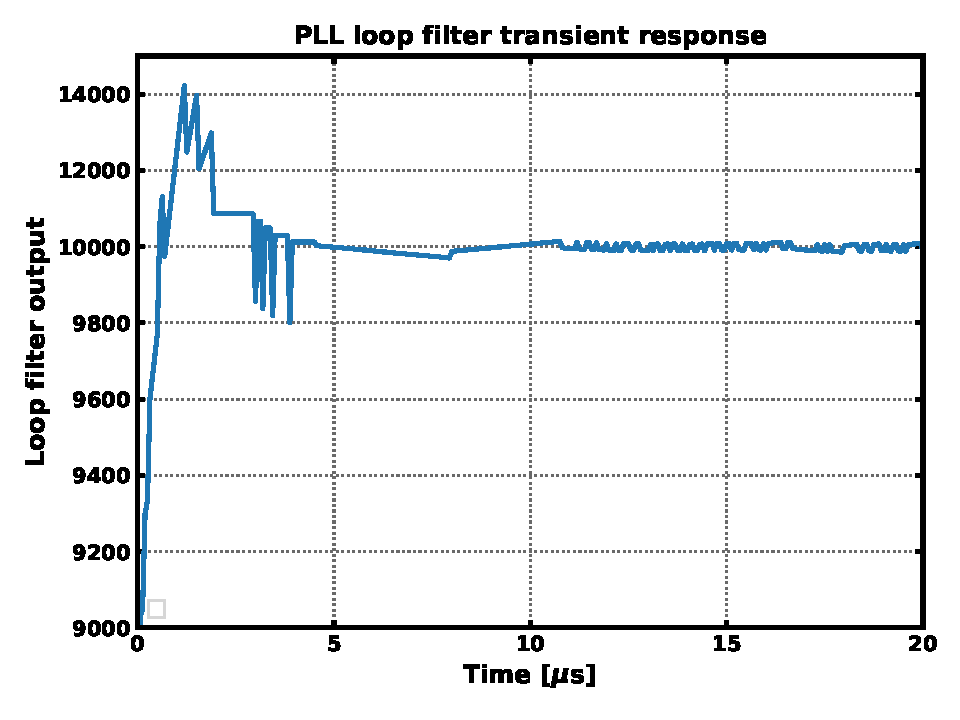
\includegraphics[width=1.0\textwidth, angle=0]{figs/trans_loop_filter_fast.pdf}
	        \caption{ }
	        \label{fig:trans_lf_fast}
	    \end{subfigure}%
	    \begin{subfigure}{0.5\textwidth}
	        \centering
	        \center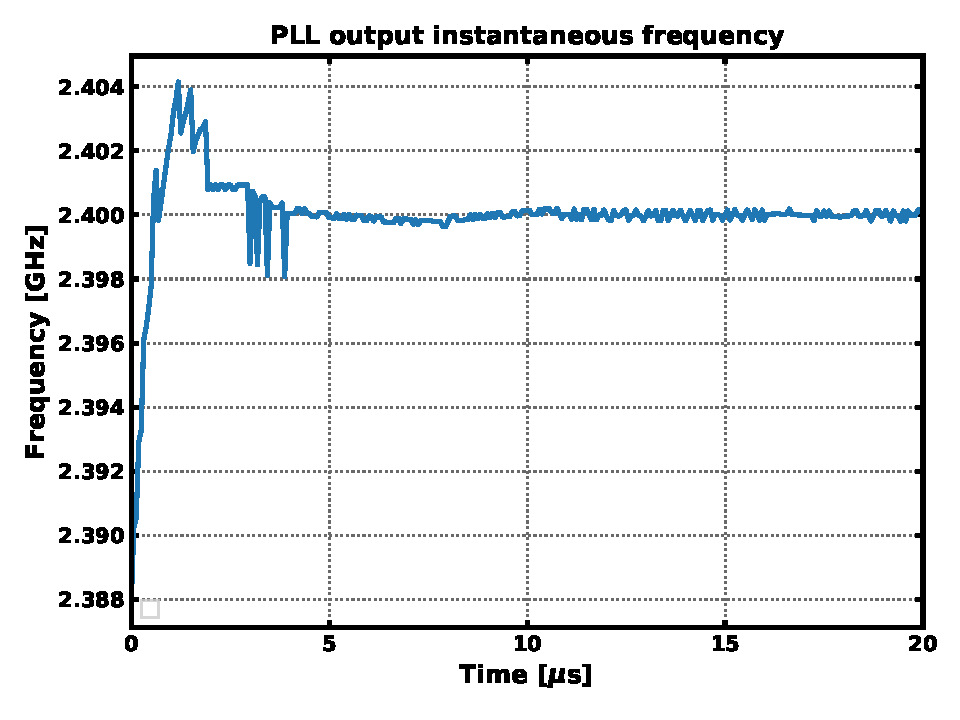
\includegraphics[width=1.0\textwidth, angle=0]{figs/trans_inst_freq_fast.pdf}
	        \caption{ }
	        \label{fig:trans_inst_freq_fast}
	    \end{subfigure}
	    % \caption{Approximate model for ring oscillator inverter delay cell.}
	    \label{fig:trans_sim1_fast}
	    \caption{Simulation with 0.5\% initial frequency error: \textbf{(a)} Loop filter transient response, \textbf{(b)} PLL output instantaneous frequency.}
	\end{figure}

	\begin{figure}[htb!]
	    \centering
	    \begin{subfigure}{0.5\textwidth}
	        \centering
	        \center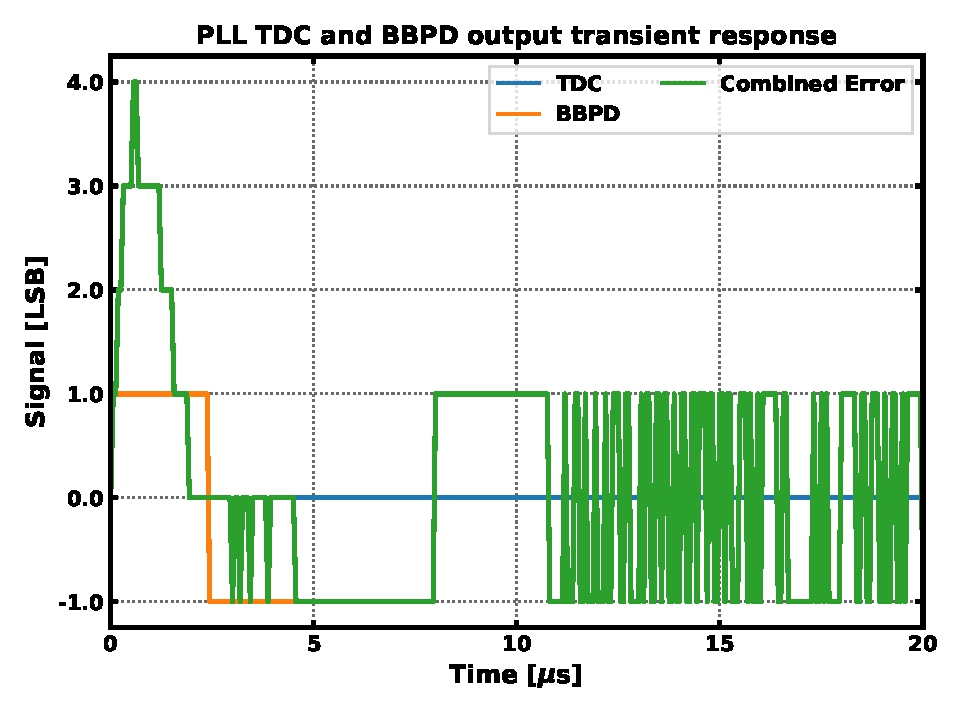
\includegraphics[width=1.0\textwidth, angle=0]{figs/trans_tdc_bbpd_fast.pdf}
	        \caption{ }
	        \label{fig:trans_det_fast}
	    \end{subfigure}%
	    \begin{subfigure}{0.5\textwidth}
	        \centering
	        \center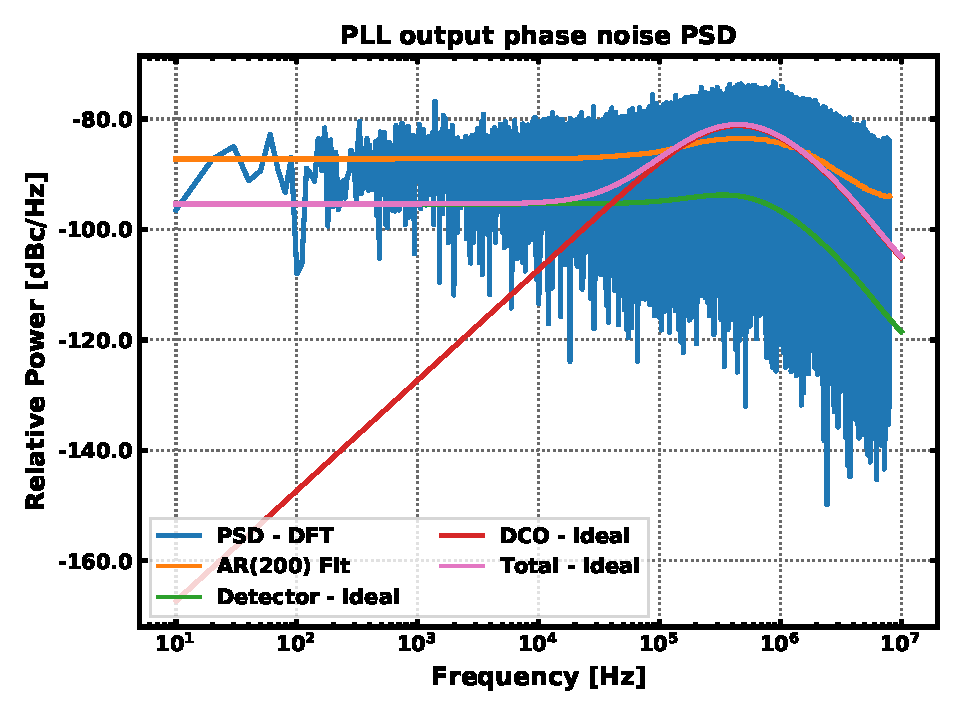
\includegraphics[width=1.0\textwidth, angle=0]{figs/trans_phase_noise_fast.pdf}
	        \caption{ }
	        \label{fig:trans_phase_noise_fast}
	    \end{subfigure}
	    % \caption{Approximate model for ring oscillator inverter delay cell.}
	    \label{fig:trans_sim2_fast}
	    \caption{Simulation with 12 MHz (0.5\%) initial frequency error: \textbf{(a)} BBPD/TDC detector responses, \textbf{(b)} PLL output phase noise power spectrum.}
	\end{figure}
\subsubsection{Approach 2: Results of Parameter Sweep and Variational Analysis}
The same parameter sweeps for $K_{DCO}$ and initial frequency error of approach 1 were applied here. In figures \ref{fig:sweep_kdco_fast} and \ref{fig:sweep_finit_fast}, the results of these sweeps are shown. The loop filter gear switching mechanism as modeled in the simulation waits a fixed time interval before switching gears, in this case chosen to be 2.0 times the estimated lock time given in table \ref{filter_params_fast_lock}. This interval has provided sufficient settling within the simulated parameter range of $K_{DCO}$ and initial frequency error that lock time stability is observed under most conditions, except under high offset for $K_{DCO}$ and initial frequency error. It was established for this simulation results that tolerance range for $K_{DCO}$ is -6950/+9750 Hz/LSB from the nominal 10000 Hz/LSB value, and the capture range is 168 MHz. Figures \ref{fig:mc_trans_fast} and \ref{fig:mc_hist_fast} demonstrate a variational simulation of the PLL using Monte-Carlo sampling, with 1000 samples. The simulation was configured to vary $K_{DCO}$ with a standard deviation of 20 \% of the nominal value, and to vary the initial starting frequency with a standard deviation of 60 MHz (2.5 \% of the final frequency). It was observed that the PLL stably locked for all simulation instances, a mean lock time of 5.96 $\mu$s was achieved. This value correlates well with the estimate of 5.52 $\mu$s from the filter design process. The upper bound for a 99\% confidence interval of lock time is 11.625 $\mu$s, thus meeting the 25$\mu$s lock time specification with considerable margin. The extracted PLL performance parameters from these simulations of this gear-switching PLL is in table \ref{simulation_params_fast}. 
	\begin{figure}[htb!]
	    \centering
	    \begin{subfigure}{0.5\textwidth}
	        \centering
	        \center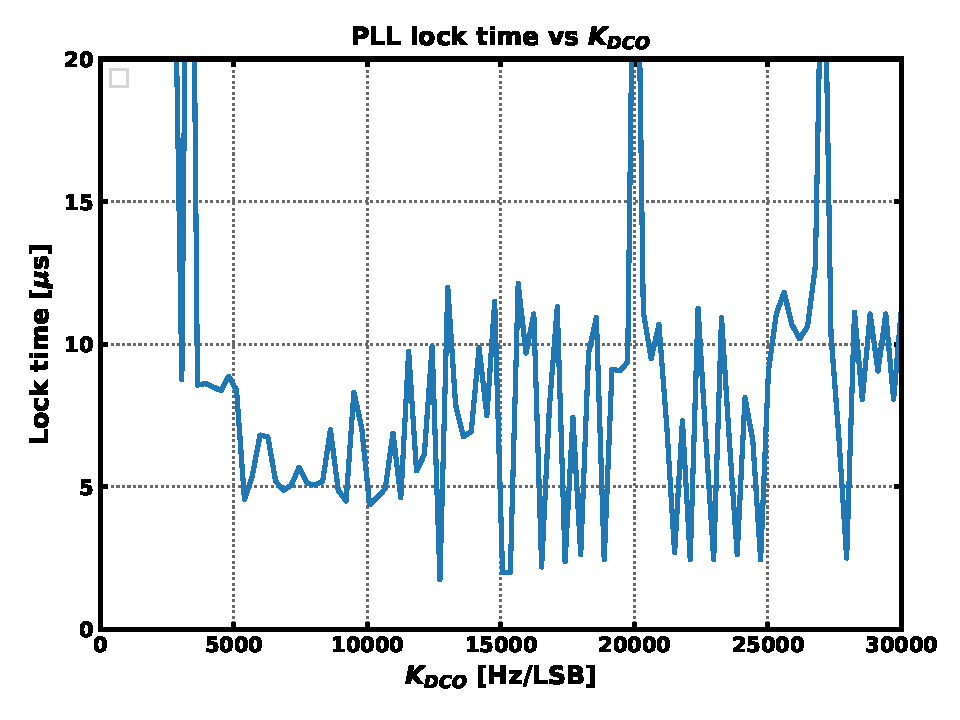
\includegraphics[width=1.0\textwidth, angle=0]{figs/_kdco_sweep_fast.pdf}
	        \caption{ }
	        \label{fig:sweep_kdco_fast}
	    \end{subfigure}%
	    \begin{subfigure}{0.5\textwidth}
	        \centering
	        \center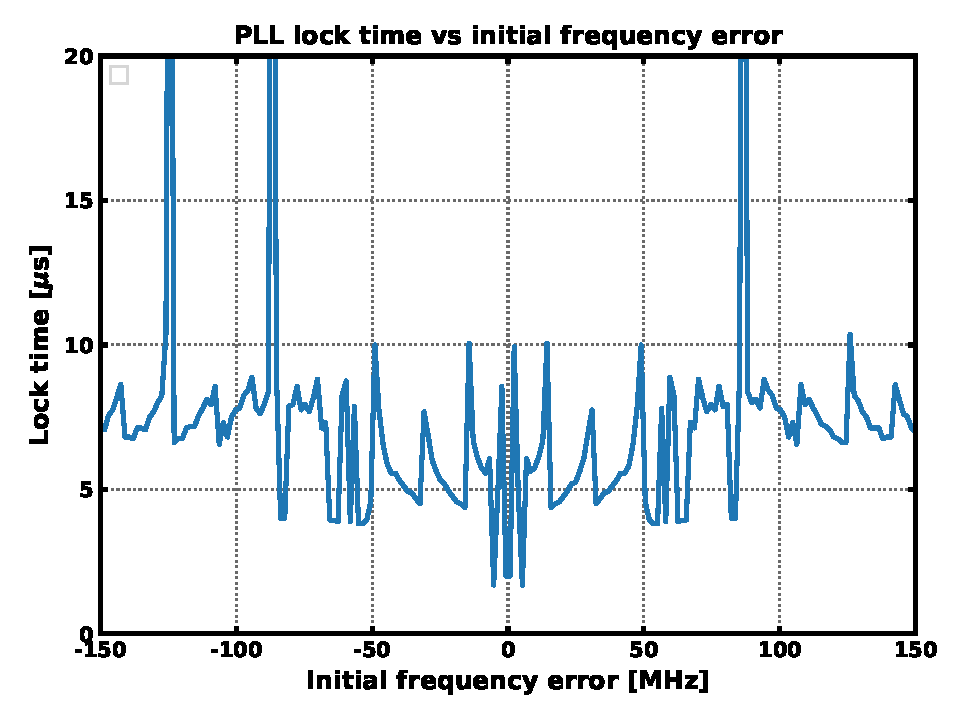
\includegraphics[width=1.0\textwidth, angle=0]{figs/finit_sweep_fast.pdf}
	        \caption{ }
	        \label{fig:sweep_finit_fast}
	    \end{subfigure}
	    % \caption{Approximate model for ring oscillator inverter delay cell.}
	    \label{fig:sweep_sim_fast}
	    \caption{\textbf{(a)} PLL lock time simulation with KDCO swept, 12 MHz (0.5\%) initial frequency error, \textbf{(b)} PLL lock time simulation with initial frequency error swept.}
	\end{figure}

	\begin{figure}[htb!]
	    \centering
	    \begin{subfigure}{0.5\textwidth}
	        \centering
	        \center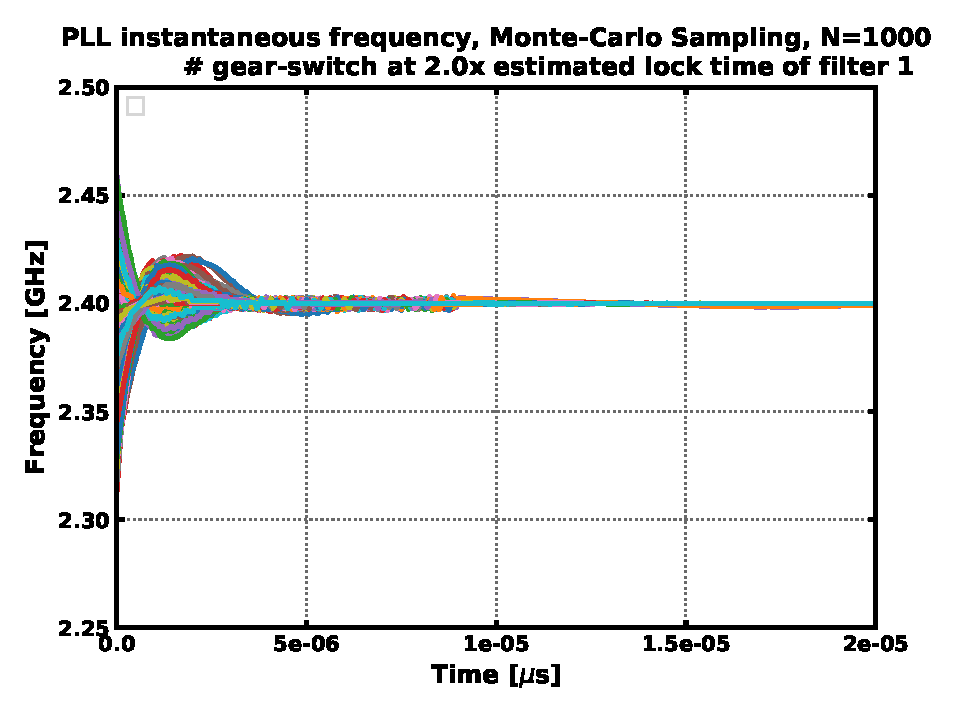
\includegraphics[width=1.0\textwidth, angle=0]{figs/mc_trans_2x.pdf}
	        \caption{ }
	        \label{fig:mc_trans_fast}
	    \end{subfigure}%
	    \begin{subfigure}{0.5\textwidth}
	        \centering
	        \center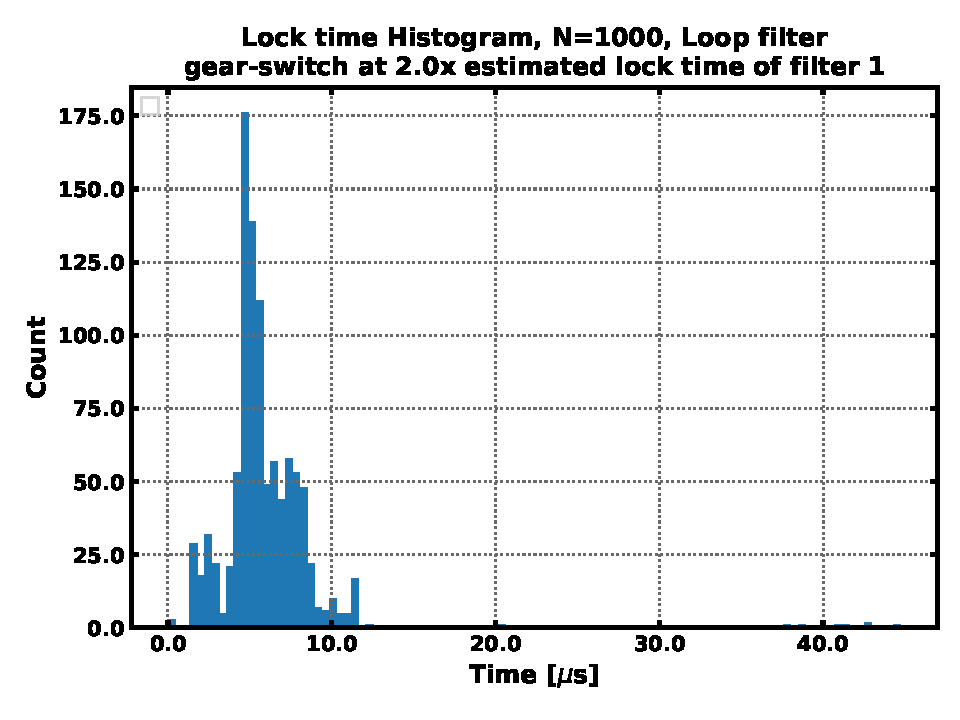
\includegraphics[width=1.0\textwidth, angle=0]{figs/mc_hist_fast_2x.pdf}
	        \caption{ }
	        \label{fig:mc_hist_fast}
	    \end{subfigure}
	    % \caption{Approximate model for ring oscillator inverter delay cell.}
	    \label{fig:mc_sim_fast}
	    \caption{Monte-Carlo simulation with 1000 samples, 20\% RMS deviation in KDCO, and 60 MHz (2.5\%) RMS deviation in initial frequency error \textbf{(a)} Frequency transient responses, \textbf{(b)} Lock time histogram.}
	\end{figure}

\begin{table}[h!]
	\centering
	\def\arraystretch{1.5}		
	\setlength\arrayrulewidth{0.75pt}
	\setlength{\tabcolsep}{1em} % for the horizontal padding
	\begin{tabular}{|l|r|l|}
		\hline 
		\rule[-1ex]{0pt}{2.5ex} \cellcolor{gray!40}\textbf{Parameter} & \cellcolor{gray!40}\textbf{Value} & \cellcolor{gray!40}\textbf{Unit }\\ 
		\hline 
		\rule[-1ex]{0pt}{2.5ex} \textbf{$K_{DCO}$ Tolerance}  & -6950/+9750 & Hz/LSB \\
		\hline 
		\rule[-1ex]{0pt}{2.5ex} \textbf{Capture range}  & 168 ($\pm 84$)& MHz\\ 
		\hline 
		\rule[-1ex]{0pt}{2.5ex} \textbf{Mean lock time}  & 5.961688& $\mu$s \\
		\hline 
		\rule[-1ex]{0pt}{2.5ex} \textbf{Lock time $\sigma$} & 3.611130 & $\mu$s\\ 
		\hline 
		\rule[-1ex]{0pt}{2.5ex} \textbf{Lock time 99 \% CI upper bound} & 11.625  & $\mu$s\\
		\hline 
		\rule[-1ex]{0pt}{2.5ex} \textbf{Residual phase modulation} & $4.367535\times10^{-2}$ & rad$^2$\\ 
		\hline 
	\end{tabular} 

	% \caption{Assigned specifications for branch line hybrid design.}
	% \label{asgn_specs}
	\caption{PLL parameters extracted from variance and parameter sweep simulations.}
	\label{simulation_params_fast}
\end{table}
\pagebreak
\subsubsection{Results Comparison of Design Approaches}
A comparison of the two design approaches shows that the PLL utilizing the gear switching results in a superior result using the design automation framework of this work. The usage of gear switching results in lower phase noise than approach 1, with total phase noise power (residual phase modulation) of 4.36$\times 10^{-2}$ rad$^2$ versus 3.37$\times 10^{-1}$ rad$^2$. Additionally, the lock time is significantly lower in the PLL with gear switching, at an average of 5.96 $\mu$s versus 19.32 $\mu$s. Therefore it has been shown that this framework offers the capability to design gear-switching PLLs with performance advantages to static loop filter PLL designs.

	% \begin{figure}[htb!]
	% 	\center\includegraphics[width=1.0\textwidth, angle=0]{figs/x.pdf}
	% 	\caption{Transient simulation of optimal design.}
	% 	\label{fig:des_ex_trans}
	% \end{figure}
	% \FloatBarrier

	% \begin{figure}[htb!]
	% 	\center\includegraphics[width=1.0\textwidth, angle=0]{figs/x.pdf}
	% 	\caption{Variation Simulation for KDCO.}
	% 	\label{fig:var_lock}
	% \end{figure}
	% \FloatBarrier

	% \begin{figure}[htb!]
	% 	\center\includegraphics[width=1.0\textwidth, angle=0]{figs/x.pdf}
	% 	\caption{Phase noise.}
	% 	\label{fig:Simulated phase noise.}
	% \end{figure}
	% \FloatBarrier

	% stability criteria - Jurys' stability criteria abs(a0) l.t. a2 for second order z-transfer \cite{xiu_li_meiners_padakanti_2004}
	% - Not phase margin based in optimization, can make stable by using stable choice of PI controller (two poles only) - poles should be in unit circle...
\FloatBarrier
\subsection{Comparison to Existing Solutions}
Due to the relative youth of all digital PLL design, and discontinuity between the continuous theory of analog PLL and digital PLL design, a smaller body of work exist pertaining to the loop filters for exclusively ADPLLs. Of the existing literature, the majority design approaches utilize discrete-time transformed PI-controller loop filters with either bang-bang phase detectors \cite{zanuso_2009}\cite{xu_abidi_2017}\cite{kratyuk_2007}\cite{safwat_ghoneima_ismail_2011} or phase-frequency detectors \cite{kumm_klingbeil_zipf_2010}\cite{chau_chen_2009}. This work takes a similar approach to the aforementioned existing works, focusing on a fixed filter architecture to limit the scope of the problem at hand, and also uses a bang-bang phase detector in its PLL architecture. This work, though, uniquely considers the optimization of digital loop filter design to use a TDC and BBPD in conjunction. Also, the approach to filter design here, which is through numerical methods to find an optimal configuration, differs from the other works that largely focus on closed-form mathematical analysis. The usage of numerical methods has allowed for implementation in this work of (a) full automation of the loop filter design process, including generation of optimal digitized filter coefficients, and (b) automatic verification through the simulator integrated into this filter design framework. These aspects of this work reduces overall implementation work for the PLL designer, and are not paralleled by any existing literature or openly available code bases. 

The criteria and motivation for loop design varies across the surveyed works. Of the surveyed works, several \cite{kratyuk_2007}\cite{kumm_klingbeil_zipf_2010}\cite{chau_chen_2009}\cite{safwat_ghoneima_ismail_2011} do not consider optimization for phase noise as this work principally does, but rather consider stability/phase margin \cite{kratyuk_2007}\cite{kumm_klingbeil_zipf_2010}\cite{safwat_ghoneima_ismail_2011}, lock time \cite{chau_chen_2009}\cite{safwat_ghoneima_ismail_2011} and even approach simplicity \cite{kumm_klingbeil_zipf_2010}. The methods that consider optimization of phase noise \cite{zanuso_2009}\cite{xu_abidi_2017} both provide a similar model of PLL dynamics based on a linearized model of the bang-bang phase detector. The design methods of the latter two works are presented with closed-form mathematical theory, using closed loop transfer function modeling to estimate phase noise from BBPD and oscillator contributions. The simulation results presented and the demonstration of correlation of their model to measurement in \cite{xu_abidi_2017}, which correlate better than that seen in this work, perhaps imply these methods provide for better optimization of BBPD-PLL phase noise than this work. The simulation methods used in those works are not described, so it is unknown if the simulations capture the presence of discrete-time and quantization-related emergent behaviors not in with their linearized PLL models. In the case of \cite{xu_abidi_2017} it appears that the loop filter is treated to be analog in nature, which differs from this work. Since the simulator used in this work accounts for full discrete-time and quantization effects, perhaps this may explain some level of observed discrepancy in the model versus simulation results compared to that in literature. 

Few of the existing works consider the implementation of the loop filter design into digital hardware, rather just provide continuous valued coefficients for the filter designs. Of those surveyed, only \cite{kumm_klingbeil_zipf_2010} provides an analysis for quantization noise in terms of spurious-free dynamic range SFDR out of the loop filter design, but lacks the connection to output phase noise. This work uniquely considers (a) the impact of quantization of the digitized filter design, in terms of filter accuracy and output phase noise, and (b) attempts to optimize the digital implementation of the filter in terms of number of bits the various components of the filter (i.e. filter coefficients, multipliers, adders) are implemented with for complexity and performance.

A final advantage of this work not observed in the surveyed literature is the integrated PLL simulator with Monte-Carlo sampling which allows for verification of the designed loop filter with accurate modeling of time-discretization and digital quantization effects. This allows for lock time, phase noise and stability to be verified on the design to ensure it meets the designer's requirements before moving onto testing with transistor level implementations and testing.

\subsection{Design Choices and Areas of Improvement}
In the design of the filter optimization in this framework for phase noise, a choice was made to only consider phase noise components resulting from detector (TDC and BBPD) noise and oscillator noise. This choice has been motivated from the reasoning that other PLL noise components, being loop filter and divider noise, can be reduced below that of these components with relative ease. In the case of the loop filter noise in a digital PLL, noise results from quantization within the filter implementation are connected with finite word effects. It shown in section \ref{lf_quant_noise_opt} that the quantization noise can be reduced considerably by increasing the number of bits used to represent data in the digital filter representation. As it was seen in figure \ref{fig:ex_pll_pn_comps}, the detector phase noise referred to the PLL output in the PLL architecture of this work is low pass with higher order roll than the TDC, thus a sufficient number of bits utilized in the loop filter implementation data words will reduce all output-referred loop filter noise components below detector noise. An optimizer was accordingly implemented in this work to select the optimal number of bits automatically for loop filter noise to be insignificant. In the case of divider noise, it is seen in the theory of section \ref{final_pn_model} in equations \ref{eq:tdc_pn_psd} and \ref{eq:div_pn_psd} that the detector noise (in this case TDC) and divider noise PSD referred to the PLL output both have a frequency dependence proportional to the closed loop PLL response, i.e. $\propto\hat{\mathrm{T}}(s)$. As demonstrated in appendix \ref{div_noise_constraint}, by constraining the output PSD of the divider to be below detector, it is found that the maximum allowed divider RMS jitter $\sigma_{tn_{div}}$ is in equation \ref{eq:max_div_jitter}, for a TDC with with M steps per reference cycle. This is observed to be equal to the time resolution of the detector, in the case of the TDC $\Delta t_{step_{TDC}}$. This shows that the divider jitter requirement is rather loose, for example with a 10 MHz reference frequency and a 1000-step resolution TDC, the maximum RMS jitter limit is 100 ps. 
\begin{equation}\label{eq:max_div_jitter}
		\sigma_{tn_{div}} < \frac{1}{\mathrm{M}f_{ref}} = \Delta t_{step_{TDC}}
\end{equation}

A further choice in the modeling and optimization of phase noise in this work was to only utilize $\propto f^{-2}$ components of oscillator phase noise from the Leeson model discussed in section \ref{dco_noise}, ignoring flicker frequency ($\propto f^{-1}$) components. The rationale for the exclusion of flicker noise components was that it is expected that flicker components of the reference oscillator will be significantly larger than the DCO contributions. Analyzing the PLL phase noise sensitivity transfer functions of section \ref{ntfs} shows that divider and reference noise is transferred to PLL output with sensitivity N$\hat{\mathrm{T}}(s)$, and DCO noise with 1-$\hat{\mathrm{T}}(s)$. The normalized PLL transfer function $\hat{\mathrm{T}}(s)$ has a zero-frequency gain of 1, i.e. $|\hat{\mathrm{T}}(0)|$ = 1. Thus, it is expected that near zero frequency, the flicker noise components of the DCO noise will be rejected as the low frequency region is the dominant flicker noise region. However, the reference flicker phase noise will be multiplied by the divider ratio N. Thus, DCO flicker contributions will be minor compared to the reference, and are not considered in the loop filter optimization code, nor the PLL behavioral simulator. Despite the significance of reference flicker noise, reference noise components are not included in the optimization and simulation processes in this work owing to reasoning that the reference noise is not easily improved with loop filter tuning. This is due to the fixed low frequency reference noise sensitivity of N$\hat{\mathrm{T}}(f) \approx N$, which will not improve flicker noise unless the bandwidth of $\hat{\mathrm{T}}(s)$ is made very small.

The loop filter design optimization in this work is limited to operating on a fixed architecture, being a proportional-integral controller with optional additional pole to compensate for closed-loop peaking. This choice was selected to limit the scope of the optimization problem to a subset for which convergence of the optimizer and stability of the designs was predictable. Furthermore, the fixed architecture allowed for simple optimization of its digital implementation by using a fixed design of second order direct-type I IIR filter section. For more generality, achieving optimal higher order filter design would require exploring a range of parallel and cascade digital filter structures to minimize finite word effects \cite{proakis_1993_x}, significantly complicating the digitization process for filter than for the fixed case. It is possible gains in performance can be achieved with higher order and unconstrained architectures, so this is a possible area of improvement for this work.

To consider the limitation of the scope of this work, the simulation and optimization here only handles integer-N PLLs, which is a shortcoming as many PLL designs require fractional-N synthesis. To increase the generality of the work by extending to fractional-N PLLs, introduction of a fractional-N behavioral divider model and a major decrease in simulation time step size (much smaller than the reference cycle time used in integer-N case of this work) is a possible improvement. Reduction of the time step is required to decrease simulation time-quantization noise effects to low enough levels for the fractional divider noise characteristics to not be overpowered \cite{perrott_2002_sim}. Such an improvement may prove to be limited by the current simulator, as overall simulation time will be increased by the factor that the simulation step is divided to support fractional-N models. Another possible improvement to consider is the implementation of a non-uniform step event-driven behavioral simulator to reduce simulation steps and thus simulation time.

\FloatBarrier
% \normalsize

	% % % % % % % % % % % % % % % % % % % % % % % % % % % % % % % % % % % % 
    \FloatBarrier

    \pagebreak
    \section{Conclusion} \label{conclusion}
    Extend to fractional-N. Loop filter design will be the same, difference is divider model.


	% % % % % % % % % % % % % % % % % % % % % % % % % % % % % % % % % % % % 
	% References
    \pagebreak
	\printbibliography


	% % % % % % % % % % % % % % % % % % % % % % % % % % % % % % % % % % % % 
	% Appendix
	\pagebreak
		\appendix

	\section{Estimating PSD with Autoregressive Model}\label{yule_walker_ar_psd}
	The following is based on \cite{proakis_1993_psd}. Given a signal x[n] whose power spectrum should be estimated, its autocorrelation sequence $r_{xx}[l]$ with lag $l$ must be computed:
	\begin{equation}
		r_{xx}[l] = \sum_{n=-\infty}^{\infty} x[n]x[n-l]
	\end{equation}
	The autoregressive model for power spectrum, with p poles, that shall be fitted is given in \ref{eq:ar_psd_eq}
	\begin{equation}\label{eq:ar_psd_eq}
		S_{XX}(f) = \left.\frac{1}{|1+\sum_{n=1}^pa_nz^{-1}|^2}\right|_{z^{-1}=e^{-j2\pi f\Delta T}}
	\end{equation}
	MMSE optimization of the distribution for coefficients $\{a_1, ..., a_p\}$ is done by solving the Yule-Walker equation in \ref{eq:yule_walker}.
	\begin{equation} \label{eq:yule_walker}
	\begin{bmatrix}
	a_1\\ 
	a_2\\
	\vdots\\
	a_p
	\end{bmatrix} = 
	-\mathbf{R}_{xx}^{-1}\mathbf{r}_{xx}=
	-\begin{bmatrix}
	r_{xx}[0] & r_{xx}[1] & \dots & r_{xx}[p-1]\\ 
	r_{xx}[1] & r_{xx}[0] & \dots & r_{xx}[p-2]\\ 
	\vdots & \vdots &  & \\
	r_{xx}[p-1] & r_{xx}[p-2] &  & r_{xx}[0]
	\end{bmatrix}^{-1}
	\begin{bmatrix}
	r_{xx}[1]\\ 
	r_{xx}[2]\\
	\vdots\\
	r_{xx}[p]
	\end{bmatrix}
	\end{equation}

	\section{Divider Noise Constraint}\label{div_noise_constraint}
		Output referred phase noise PSD of TDC:
		\begin{equation}
			S_{\Phi n_{TDC,out}} = \frac{1}{12 f_{ref}}\left|2\pi\frac{N}{M} G(f) \right|^2
		\end{equation}
		Output referred phase noise PSD of divider:
		\begin{equation}
			S_{\Phi n_{div, out}} = f_{ref} \left|2\pi N \sigma_{tn_{div}} G(f)\right|^2
		\end{equation}
		The output-referred phase noise for the TDC and divider have the same frequency dependence. So by setting $S_{\Phi n_{div, out}} < S_{\Phi n_{TDC,out}}$, a constraint to force PLL output divider less than TDC noise can be found:
		\begin{equation}
			\sigma_{tn_{div}} < \frac{1}{\mathrm{M}f_{ref}} = \Delta t_{step_{TDC}}
		\end{equation}
		Must simply ensure that jitter of divider is much less than TDC resolution, which is a reasonable demand. Thus, it is reasonable to ignore divider noise in the phase noise optimization if divider noise can reasonably be made insignificant in the overall output phase noise.

\vspace{-0.8em}\center$ \square $
	% \section{Oscillator phase noise due to thermal noise}\label{osc_pn_additive_append}


	% \begin{figure}[htb!]
	% 	\center\fontfamily{\sfdefault}\selectfont
% XCircuit output "dco_noise.tex" for LaTeX input from dco_noise.ps
\def\putbox#1#2#3#4{\makebox[0.00000in][l]{\makebox[#1][l]{}\raisebox{\baselineskip}[0.00000in][0.00000in]{\raisebox{#2}[0.00000in][0.00000in]{\scalebox{#3}{#4}}}}}
\def\rightbox#1{\makebox[0.00000in][r]{#1}}
\def\centbox#1{\makebox[0.00000in]{#1}}
\def\topbox#1{\raisebox{-0.60\baselineskip}[0.00000in][0.00000in]{#1}}
\def\midbox#1{\raisebox{-0.20\baselineskip}[0.00000in][0.00000in]{#1}}
   \scalebox{1}{
   \normalsize
   \parbox{3.56562in}{
   \includegraphics[scale=0.70000]{./figs/dco_noise.pdf}\\
   % translate x=-384 y=320 scale 0.38
   \putbox{1.02900in}{0.39200in}{0.96}{u[n]}%
   \putbox{1.48400in}{0.24500in}{0.96}{$\frac{2\pi K_{DCO}T}{1-z^{-1}}$}%
   \putbox{2.66700in}{0.34300in}{0.96}{$\Phi_{out}$[n]}%
   \putbox{0.78400in}{0.60900in}{0.96}{q$_{OTW}$[n]}%
   \putbox{0.18200in}{0.37800in}{0.96}{$\hat{\textnormal{u}}$[n]}%
   \putbox{2.54800in}{0.62300in}{0.96}{$\Phi_{n_{DCO}}$[n]}%
   } % close 'parbox'
   } % close 'scalebox'
   \vspace{-\baselineskip} % this is not necessary, but looks better
\fontfamily{\rmdefault}\selectfont

	% 	\caption{DCO additive noise model.}
	% 	\label{fig:dco_noise2}
	% \end{figure}
	% \FloatBarrier

	%  Oscillator phase noise due to stochastic and uncorrelated circuit and supply noise can be analyzed as additive voltage disturbance $\delta v_n$ with variance $\sigma_{v_n}^2$ to the oscillator waveform $V_{osc}$ at any given time.  In a stable, noiseless oscillator, amplitude is inherently tied to signal phase, i.e. $V_{osc}(\Phi=\omega t)$. With additive noise, given $\frac{dV_{osc}(\Phi)}{d\Phi}$ is finite $\forall$t, a small voltage disturbance from noise $\delta v_{n}$ will be coupled as a disturbance $\delta\Phi_{n}$ in the oscillator phase, shown in figure \ref{fig:aperture_noise}. The phase evolution of the noisy oscillator for an infinitesimal time increment $\delta t$  with such a disturbance is:
	%  \begin{equation}
	% 	\Phi_{out}(t+\delta t) = \Phi_{out}(t) + \delta\Phi_n + \omega_{osc}\delta t \label{eq:rwalk_ph}
	%  \end{equation}

	% \begin{figure}[htb!]
	% 	\center\fontfamily{\sfdefault}\selectfont
% XCircuit output "aperture_noise.tex" for LaTeX input from aperture_noise.ps
\def\putbox#1#2#3#4{\makebox[0.00000in][l]{\makebox[#1][l]{}\raisebox{\baselineskip}[0.00000in][0.00000in]{\raisebox{#2}[0.00000in][0.00000in]{\scalebox{#3}{#4}}}}}
\def\rightbox#1{\makebox[0.00000in][r]{#1}}
\def\centbox#1{\makebox[0.00000in]{#1}}
\def\topbox#1{\raisebox{-0.60\baselineskip}[0.00000in][0.00000in]{#1}}
\def\midbox#1{\raisebox{-0.20\baselineskip}[0.00000in][0.00000in]{#1}}
   \scalebox{1}{
   \normalsize
   \parbox{2.24062in}{
   \includegraphics[scale=0.90000]{./figs/aperture_noise.pdf}\\
   % translate x=-108 y=240 scale 0.38
   \putbox{1.87200in}{0.16200in}{0.96}{\rotatebox{-360}{$\Phi$}}%
   \putbox{0.07200in}{1.40400in}{0.96}{V$_{out}$}%
   \putbox{0.63000in}{1.13400in}{0.96}{$\sigma_{v_n}$}%
   \putbox{0.61200in}{0.40500in}{0.96}{$\sigma_{\Phi_n}$}%
   \putbox{0.05400in}{1.06200in}{0.60}{Thermal }%
   \putbox{0.12600in}{0.97200in}{0.60}{noise}%
   \putbox{0.71100in}{0.14400in}{0.60}{Phase }%
   \putbox{0.72900in}{0.05400in}{0.60}{noise}%
   \putbox{1.58400in}{0.14400in}{0.60}{\rotatebox{-360}{$2\pi$}}%
   \putbox{0.40500in}{0.14400in}{0.60}{$0$}%
   } % close 'parbox'
   } % close 'scalebox'
   \vspace{-\baselineskip} % this is not necessary, but looks better
\fontfamily{\rmdefault}\selectfont

	% 	\caption{Voltage to phase noise conversion.}
	% 	\label{fig:aperture_noise}
	% \end{figure}
	% \FloatBarrier
	%   Assuming $\delta v_n$ is Gaussian white noise, $\delta\Phi_{n}$ is sampled stochastically at any instant based on the probability distribution \ref{eq:osc_rw_dist}, dependent on the current oscillator phase $\Phi_{out}$ and the noiseless voltage-phase relation $V_{osc}(\Phi)$. It will be assumed that like the source noise $\delta v_n$, $\delta\Phi_{n}$ is white spectrum.
	%  \begin{equation}
	%  	P(\delta\Phi_{n}|\Phi_{out}) = \text{Norm}\left(\mu=0, \sigma=\sigma_{v_n}\left(\left.\frac{dV_{osc}(\Phi)}{d\Phi}\right\vert_{\Phi=\Phi_{out}}\right)^{-1}\right) \label{eq:osc_rw_dist}
	%  \end{equation} 
	% Spectral analysis of the noisy oscillator phase can be made utilizing discrete time-modeling. Converting \ref{eq:rwalk_ph} into a sampled signal with time step $\delta t$ 
	% \begin{equation}
	% 	\Phi_{out}[n+1] = \Phi_{out}[n] + \omega_{osc}\delta t + \delta\Phi_n[n|\Phi_{out}[n]]
	% \end{equation}
	% Computing the z-transform, and splitting the result into the oscillation $\Phi_{osc}$ and phase noise $\Phi_{n}$ components:
	% \begin{equation}
	% 	\Phi_{out}(z) = \frac{\omega_{osc}\delta t}{z-1} + \frac{\delta\Phi_n(z)}{z-1} = \Phi_{osc}(z) + \Phi_{n}(z)
	% \end{equation}
	% \begin{equation}
	% 	\Rightarrow \Phi_{n}(z) = \frac{\delta\Phi_n(z)}{z-1} \label{eq:z_osc_pn}
	% \end{equation}
	% Application of the bilinear transform to \ref{eq:z_osc_pn} can be used to approximate the continuous phase noise spectrum, if $s=j\omega$
	% \begin{equation}
	% 	\Phi_{n}(s) = \left.\Phi_{n}(z)\right\vert_{z=1-s\delta t} = \left.\frac{\delta\Phi_n(z)}{z-1}\right\vert_{z=1+s\delta t} = \frac{\delta\Phi_n(s)}{s\delta t}
	% \end{equation}
	% The phase noise PSD is therefore:
	% \begin{equation}
	% 	S_{\Phi n_{DCO}}(f)= \lim_{\Delta T\rightarrow\infty}\frac{1}{\Delta T}\left|\frac{\delta\Phi_n(j2\pi f)}{j2\pi f \delta t}*\mathcal{F}\left\{\text{rect}\left(\frac{t}{\Delta t}\right)\right\}\right|^2  =  \frac{S_{0\Phi n_{DCO}}}{f^2}
	% \end{equation}
	% Following that the phase disturbance signal $\delta\Phi_{n}(t)$ is white spectrum, a constant value for its PSD $S_{0\Phi n_{DCO}}$ can be defined. The value for $S_{0\Phi n_{DCO}}$ is highly dependent on implementation and is best extracted by means of curve fitting simulation or physical measurement.



\end{document}